\subsection{Exclusivity Cuts}\label{sec:exclusivity}
The electron, proton and pion define the deuteron-reference missing mass $M_{X,d}^2=(k+P_d-k'-p_p-p_\pi)^2$ and full spatial missing momentum. Calibration is performed in the original 24 bins, separately for the three RGB periods and RGC Su22, with RGC Fa22+Sp23 pooled for window determination. Each RGC control target receives the same windows as ND$_3$ in its period. Period identities and luminosities remain separate.
A Gaussian spectator-proton peak plus nonnegative linear background defines the mass interval $\mu_M\pm2\sigma_M$. After this cut, a gamma signal plus higher-mode gamma tail describes missing momentum. The selected interval is the signal's central 95.45\% probability interval. A quadratic mass background, a varied tail shape and doubled histogram widths provide diagnostic comparisons. Unresolved Su22 shapes can be transferred from the Fa22+Sp23 reference with documented donor corrections. The signed pion-angle residual is a closure plot and is not an additional cut.
The relaxed sample is recalibrated before the three-bin target refit. All selected events retain their original fine-bin exclusivity windows. Current windows and any reference assistance are retained in the release metadata. The figures below show the new calibration, replacing the earlier sample's fits.
\clearpage
\begin{longtable}{rrrrrl}
\caption{Current exclusivity windows for RGB\_spring2020. Mass-squared boundaries are in GeV$^2$ and missing-momentum boundaries are in GeV.}\\
\toprule Bin & $M^2_{\min}$ & $M^2_{\max}$ & $p_{\min}$ & $p_{\max}$ & Shape source\\\midrule\endhead
1 & 0.7529 & 1.1150 & 0.0244 & 0.2456 & independent\\
2 & 0.7852 & 1.1195 & 0.0263 & 0.2684 & independent\\
3 & 0.7699 & 1.1135 & 0.0275 & 0.2572 & independent\\
4 & 0.7634 & 1.1294 & 0.0292 & 0.2736 & independent\\
5 & 0.7373 & 1.1443 & 0.0307 & 0.2844 & independent\\
6 & 0.7483 & 1.1379 & 0.0290 & 0.2989 & independent\\
7 & 0.7361 & 1.1436 & 0.0254 & 0.2615 & independent\\
8 & 0.7962 & 1.1357 & 0.0291 & 0.2880 & independent\\
9 & 0.7930 & 1.1376 & 0.0289 & 0.2695 & independent\\
10 & 0.7989 & 1.1137 & 0.0265 & 0.2556 & independent\\
11 & 0.7844 & 1.1151 & 0.0278 & 0.2439 & independent\\
12 & 0.8106 & 1.1023 & 0.0278 & 0.2385 & independent\\
13 & 0.7283 & 1.1687 & 0.0268 & 0.2654 & independent\\
14 & 0.7674 & 1.1619 & 0.0289 & 0.2938 & independent\\
15 & 0.8046 & 1.1247 & 0.0287 & 0.2780 & independent\\
16 & 0.8071 & 1.1201 & 0.0279 & 0.2841 & independent\\
17 & 0.7979 & 1.1257 & 0.0270 & 0.2552 & independent\\
18 & 0.7828 & 1.1403 & 0.0290 & 0.2671 & independent\\
19 & 0.7219 & 1.1967 & 0.0265 & 0.2743 & independent\\
20 & 0.7502 & 1.2018 & 0.0290 & 0.2939 & independent\\
21 & 0.7740 & 1.1569 & 0.0291 & 0.2925 & independent\\
22 & 0.7836 & 1.1415 & 0.0286 & 0.2918 & independent\\
23 & 0.7795 & 1.1512 & 0.0286 & 0.2805 & independent\\
24 & 0.7693 & 1.1718 & 0.0296 & 0.2946 & independent\\
\bottomrule\end{longtable}
\clearpage
\begin{longtable}{rrrrrl}
\caption{Current exclusivity windows for RGC\_fall2022\_spring2023. Mass-squared boundaries are in GeV$^2$ and missing-momentum boundaries are in GeV.}\\
\toprule Bin & $M^2_{\min}$ & $M^2_{\max}$ & $p_{\min}$ & $p_{\max}$ & Shape source\\\midrule\endhead
1 & 0.7138 & 1.1728 & 0.0408 & 0.4729 & independent\\
2 & 0.7627 & 1.1786 & 0.0358 & 0.4236 & independent\\
3 & 0.8015 & 1.1453 & 0.0394 & 0.3993 & independent\\
4 & 0.7833 & 1.1448 & 0.0390 & 0.4039 & independent\\
5 & 0.7475 & 1.1051 & 0.0370 & 0.3952 & independent\\
6 & 0.7985 & 1.1388 & 0.0381 & 0.4168 & independent\\
7 & 0.7132 & 1.1781 & 0.0364 & 0.3946 & independent\\
8 & 0.7810 & 1.1752 & 0.0419 & 0.4091 & independent\\
9 & 0.8056 & 1.1527 & 0.0376 & 0.3918 & independent\\
10 & 0.7864 & 1.1557 & 0.0392 & 0.3803 & independent\\
11 & 0.7670 & 1.1716 & 0.0395 & 0.3962 & independent\\
12 & 0.8216 & 1.1473 & 0.0398 & 0.3811 & independent\\
13 & 0.7215 & 1.1895 & 0.0359 & 0.3629 & independent\\
14 & 0.7656 & 1.2013 & 0.0407 & 0.3987 & independent\\
15 & 0.8146 & 1.1670 & 0.0428 & 0.4275 & independent\\
16 & 0.7977 & 1.1804 & 0.0434 & 0.4530 & independent\\
17 & 0.8416 & 1.1264 & 0.0406 & 0.4275 & independent\\
18 & 0.8120 & 1.1523 & 0.0423 & 0.4464 & independent\\
19 & 0.7473 & 1.1870 & 0.0333 & 0.3829 & independent\\
20 & 0.7722 & 1.2074 & 0.0378 & 0.3817 & independent\\
21 & 0.7922 & 1.1795 & 0.0400 & 0.3711 & independent\\
22 & 0.7972 & 1.1651 & 0.0400 & 0.3948 & independent\\
23 & 0.8186 & 1.1490 & 0.0409 & 0.3987 & independent\\
24 & 0.7972 & 1.1477 & 0.0418 & 0.4259 & independent\\
\bottomrule\end{longtable}
\clearpage
\begin{longtable}{rrrrrl}
\caption{Current exclusivity windows for RGB\_fall2019. Mass-squared boundaries are in GeV$^2$ and missing-momentum boundaries are in GeV.}\\
\toprule Bin & $M^2_{\min}$ & $M^2_{\max}$ & $p_{\min}$ & $p_{\max}$ & Shape source\\\midrule\endhead
1 & 0.7469 & 1.1264 & 0.0237 & 0.2422 & independent\\
2 & 0.7747 & 1.1224 & 0.0252 & 0.2535 & independent\\
3 & 0.7481 & 1.1222 & 0.0271 & 0.2547 & independent\\
4 & 0.7249 & 1.1232 & 0.0281 & 0.2679 & independent\\
5 & 0.7036 & 1.1204 & 0.0293 & 0.2670 & independent\\
6 & 0.7946 & 1.0648 & 0.0255 & 0.2917 & independent\\
7 & 0.7285 & 1.1327 & 0.0240 & 0.2471 & independent\\
8 & 0.7609 & 1.1185 & 0.0257 & 0.2574 & independent\\
9 & 0.7471 & 1.1110 & 0.0268 & 0.2606 & independent\\
10 & 0.7663 & 1.0688 & 0.0252 & 0.2463 & independent\\
11 & 0.7257 & 1.0897 & 0.0278 & 0.2479 & independent\\
12 & 0.7484 & 1.0631 & 0.0278 & 0.2407 & independent\\
13 & 0.7041 & 1.1597 & 0.0253 & 0.2564 & independent\\
14 & 0.7476 & 1.1437 & 0.0269 & 0.2804 & independent\\
15 & 0.7585 & 1.1296 & 0.0289 & 0.2846 & independent\\
16 & 0.7530 & 1.0851 & 0.0270 & 0.2511 & independent\\
17 & 0.7636 & 1.0991 & 0.0270 & 0.2550 & independent\\
18 & 0.7289 & 1.0987 & 0.0282 & 0.2393 & independent\\
19 & 0.7016 & 1.1839 & 0.0275 & 0.2545 & independent\\
20 & 0.6963 & 1.2490 & 0.0296 & 0.3310 & independent\\
21 & 0.7678 & 1.1305 & 0.0283 & 0.2789 & independent\\
22 & 0.7270 & 1.1157 & 0.0295 & 0.2688 & independent\\
23 & 0.7523 & 1.1071 & 0.0253 & 0.2738 & independent\\
24 & 0.7109 & 1.1201 & 0.0275 & 0.2834 & independent\\
\bottomrule\end{longtable}
\clearpage
\begin{longtable}{rrrrrl}
\caption{Current exclusivity windows for RGB\_spring2019. Mass-squared boundaries are in GeV$^2$ and missing-momentum boundaries are in GeV.}\\
\toprule Bin & $M^2_{\min}$ & $M^2_{\max}$ & $p_{\min}$ & $p_{\max}$ & Shape source\\\midrule\endhead
1 & 0.7208 & 1.0844 & 0.0226 & 0.2266 & independent\\
2 & 0.7460 & 1.0883 & 0.0241 & 0.2408 & independent\\
3 & 0.7306 & 1.0828 & 0.0252 & 0.2452 & independent\\
4 & 0.7264 & 1.0954 & 0.0250 & 0.2568 & independent\\
5 & 0.7206 & 1.0839 & 0.0258 & 0.2660 & independent\\
6 & 0.7155 & 1.0825 & 0.0275 & 0.2577 & independent\\
7 & 0.7159 & 1.1046 & 0.0236 & 0.2447 & independent\\
8 & 0.7649 & 1.0888 & 0.0252 & 0.2522 & independent\\
9 & 0.7514 & 1.0947 & 0.0254 & 0.2469 & independent\\
10 & 0.7804 & 1.0709 & 0.0247 & 0.2305 & independent\\
11 & 0.7580 & 1.0749 & 0.0254 & 0.2404 & independent\\
12 & 0.7566 & 1.0836 & 0.0263 & 0.2402 & independent\\
13 & 0.6976 & 1.1448 & 0.0256 & 0.2503 & independent\\
14 & 0.7392 & 1.1224 & 0.0265 & 0.2734 & independent\\
15 & 0.7690 & 1.0822 & 0.0252 & 0.2614 & independent\\
16 & 0.7658 & 1.0848 & 0.0253 & 0.2470 & independent\\
17 & 0.7855 & 1.0603 & 0.0244 & 0.2274 & independent\\
18 & 0.7479 & 1.0902 & 0.0250 & 0.2369 & independent\\
19 & 0.6872 & 1.1822 & 0.0253 & 0.2626 & independent\\
20 & 0.7116 & 1.1676 & 0.0271 & 0.2806 & independent\\
21 & 0.7156 & 1.1292 & 0.0272 & 0.2850 & independent\\
22 & 0.7484 & 1.0824 & 0.0255 & 0.2695 & independent\\
23 & 0.7100 & 1.1246 & 0.0280 & 0.2772 & independent\\
24 & 0.7391 & 1.0948 & 0.0256 & 0.2522 & independent\\
\bottomrule\end{longtable}
\clearpage
\begin{longtable}{rrrrrl}
\caption{Current exclusivity windows for RGC\_summer2022. Mass-squared boundaries are in GeV$^2$ and missing-momentum boundaries are in GeV.}\\
\toprule Bin & $M^2_{\min}$ & $M^2_{\max}$ & $p_{\min}$ & $p_{\max}$ & Shape source\\\midrule\endhead
1 & 0.7179 & 1.1481 & 0.0384 & 0.4861 & independent\\
2 & 0.7799 & 1.0820 & 0.0319 & 0.3513 & independent\\
3 & 0.7768 & 1.0942 & 0.0338 & 0.3430 & independent\\
4 & 0.8709 & 0.9944 & 0.0351 & 0.2998 & independent\\
5 & 0.7247 & 1.0597 & 0.0376 & 0.3639 & reference-assisted\\
6 & 0.7752 & 1.0939 & 0.0361 & 0.3855 & reference-assisted\\
7 & 0.6944 & 1.1840 & 0.0372 & 0.4334 & independent\\
8 & 0.7725 & 1.1406 & 0.0395 & 0.4215 & independent\\
9 & 0.7959 & 1.1219 & 0.0385 & 0.4544 & independent\\
10 & 0.7014 & 1.1723 & 0.0375 & 0.3928 & independent\\
11 & 0.8130 & 1.0392 & 0.0310 & 0.2811 & independent\\
12 & 0.7978 & 1.1029 & 0.0360 & 0.3829 & reference-assisted\\
13 & 0.6840 & 1.1806 & 0.0343 & 0.3783 & independent\\
14 & 0.7437 & 1.1673 & 0.0383 & 0.4035 & independent\\
15 & 0.7501 & 1.0847 & 0.0408 & 0.4599 & independent\\
16 & 0.8007 & 1.0835 & 0.0395 & 0.4247 & independent\\
17 & 0.7518 & 1.1737 & 0.0443 & 0.5015 & independent\\
18 & 0.8382 & 0.9178 & 0.0320 & 0.2380 & independent\\
19 & 0.6775 & 1.1949 & 0.0322 & 0.3629 & independent\\
20 & 0.6996 & 1.2301 & 0.0381 & 0.3963 & independent\\
21 & 0.7574 & 1.1485 & 0.0399 & 0.3705 & independent\\
22 & 0.7746 & 1.1140 & 0.0418 & 0.4060 & independent\\
23 & 0.7537 & 1.1025 & 0.0408 & 0.4184 & independent\\
24 & 0.7123 & 1.2052 & 0.0465 & 0.4610 & independent\\
\bottomrule\end{longtable}

\begin{figure}[p]\centering
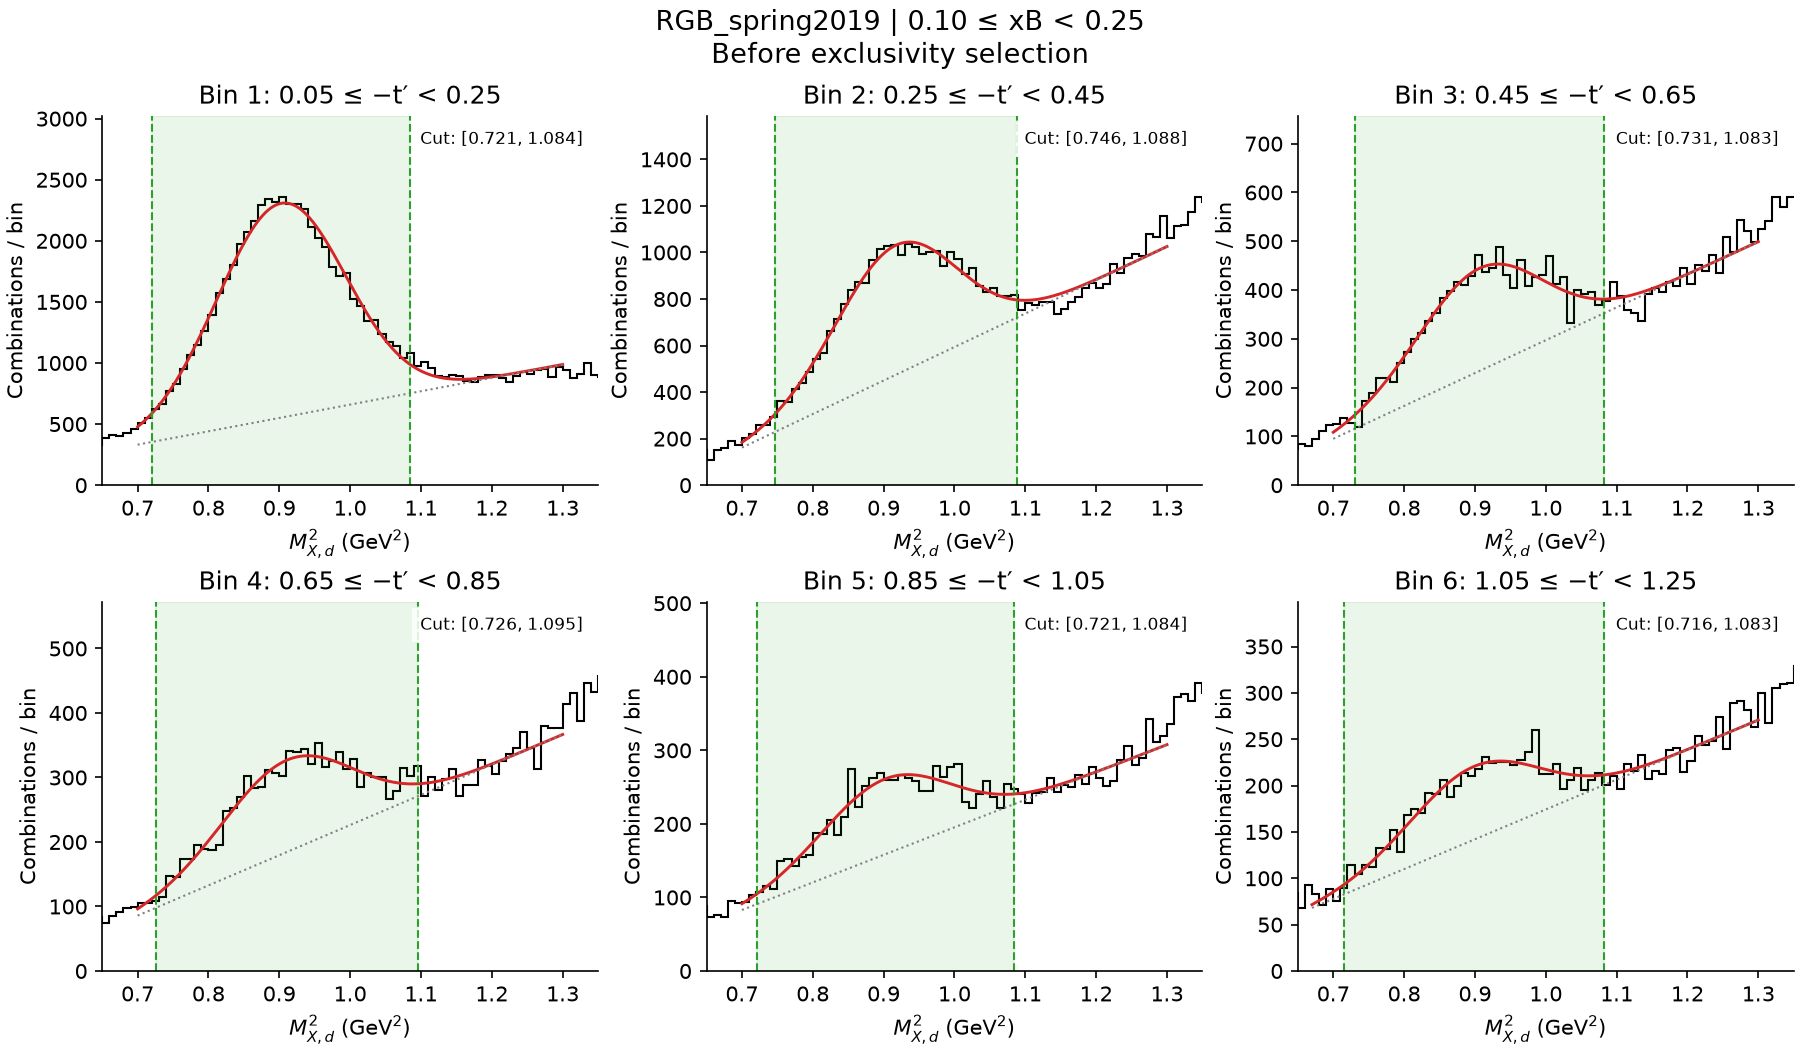
\includegraphics[width=\linewidth]{figures/channel_selection/exclusivity/rgb_sp19_mass_xb1.png}
\caption{RGB\_spring2019: deuteron-reference missing-mass-squared fits in $x_B$ interval 1. The panels retain the six fine selection bins.}\label{fig:new_excl_rgb_sp19_mass1}
\end{figure}
\clearpage
\begin{figure}[p]\centering
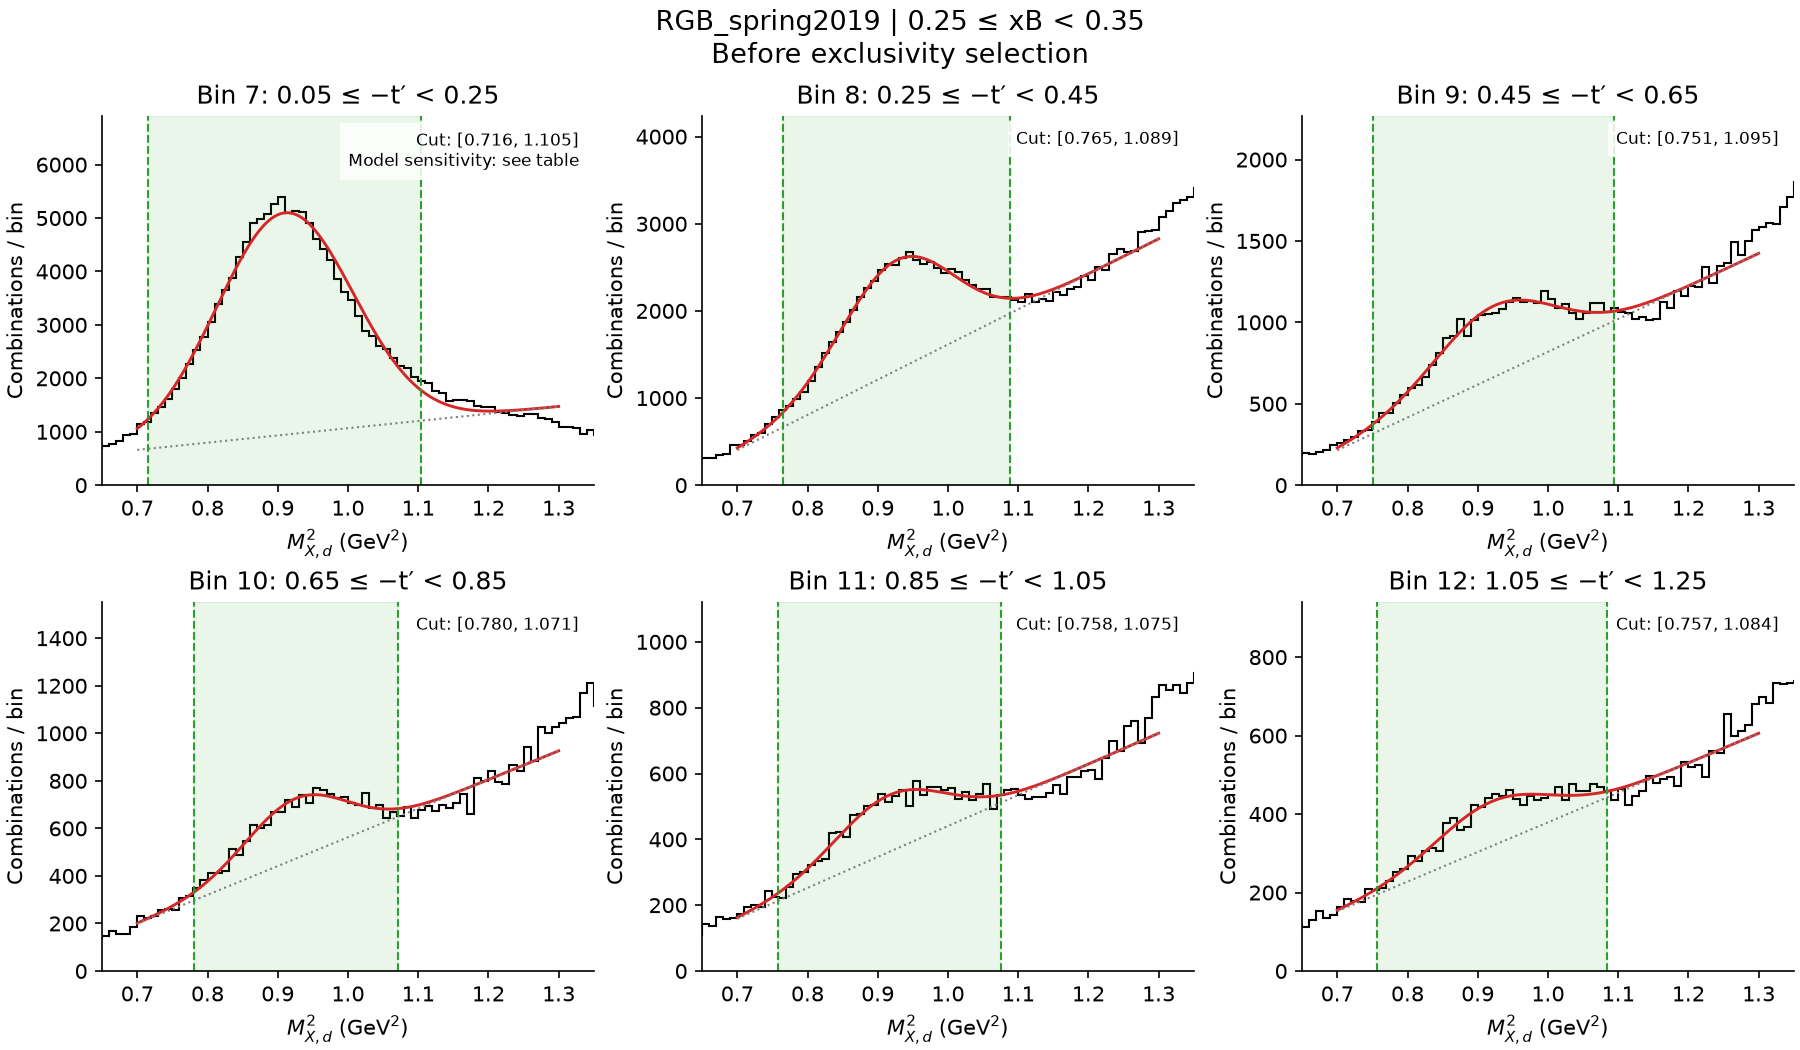
\includegraphics[width=\linewidth]{figures/channel_selection/exclusivity/rgb_sp19_mass_xb2.png}
\caption{RGB\_spring2019: deuteron-reference missing-mass-squared fits in $x_B$ interval 2. The panels retain the six fine selection bins.}\label{fig:new_excl_rgb_sp19_mass2}
\end{figure}
\clearpage
\begin{figure}[p]\centering
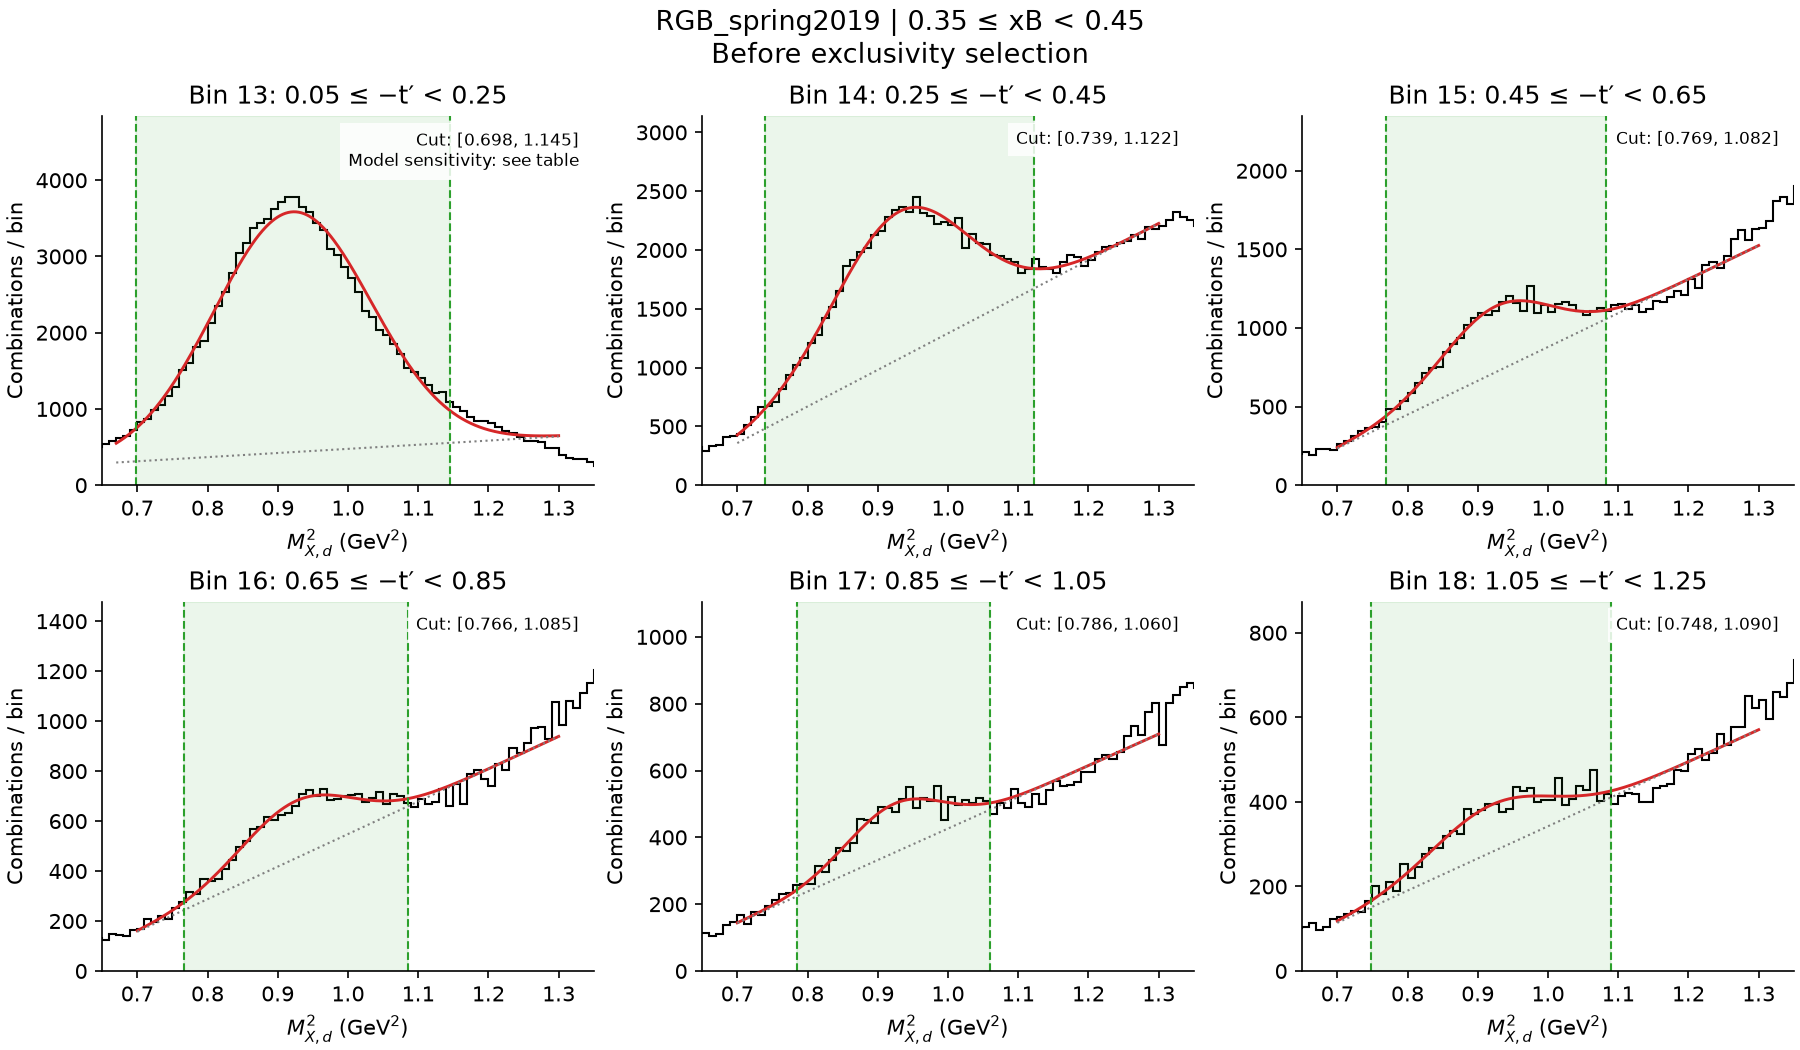
\includegraphics[width=\linewidth]{figures/channel_selection/exclusivity/rgb_sp19_mass_xb3.png}
\caption{RGB\_spring2019: deuteron-reference missing-mass-squared fits in $x_B$ interval 3. The panels retain the six fine selection bins.}\label{fig:new_excl_rgb_sp19_mass3}
\end{figure}
\clearpage
\begin{figure}[p]\centering
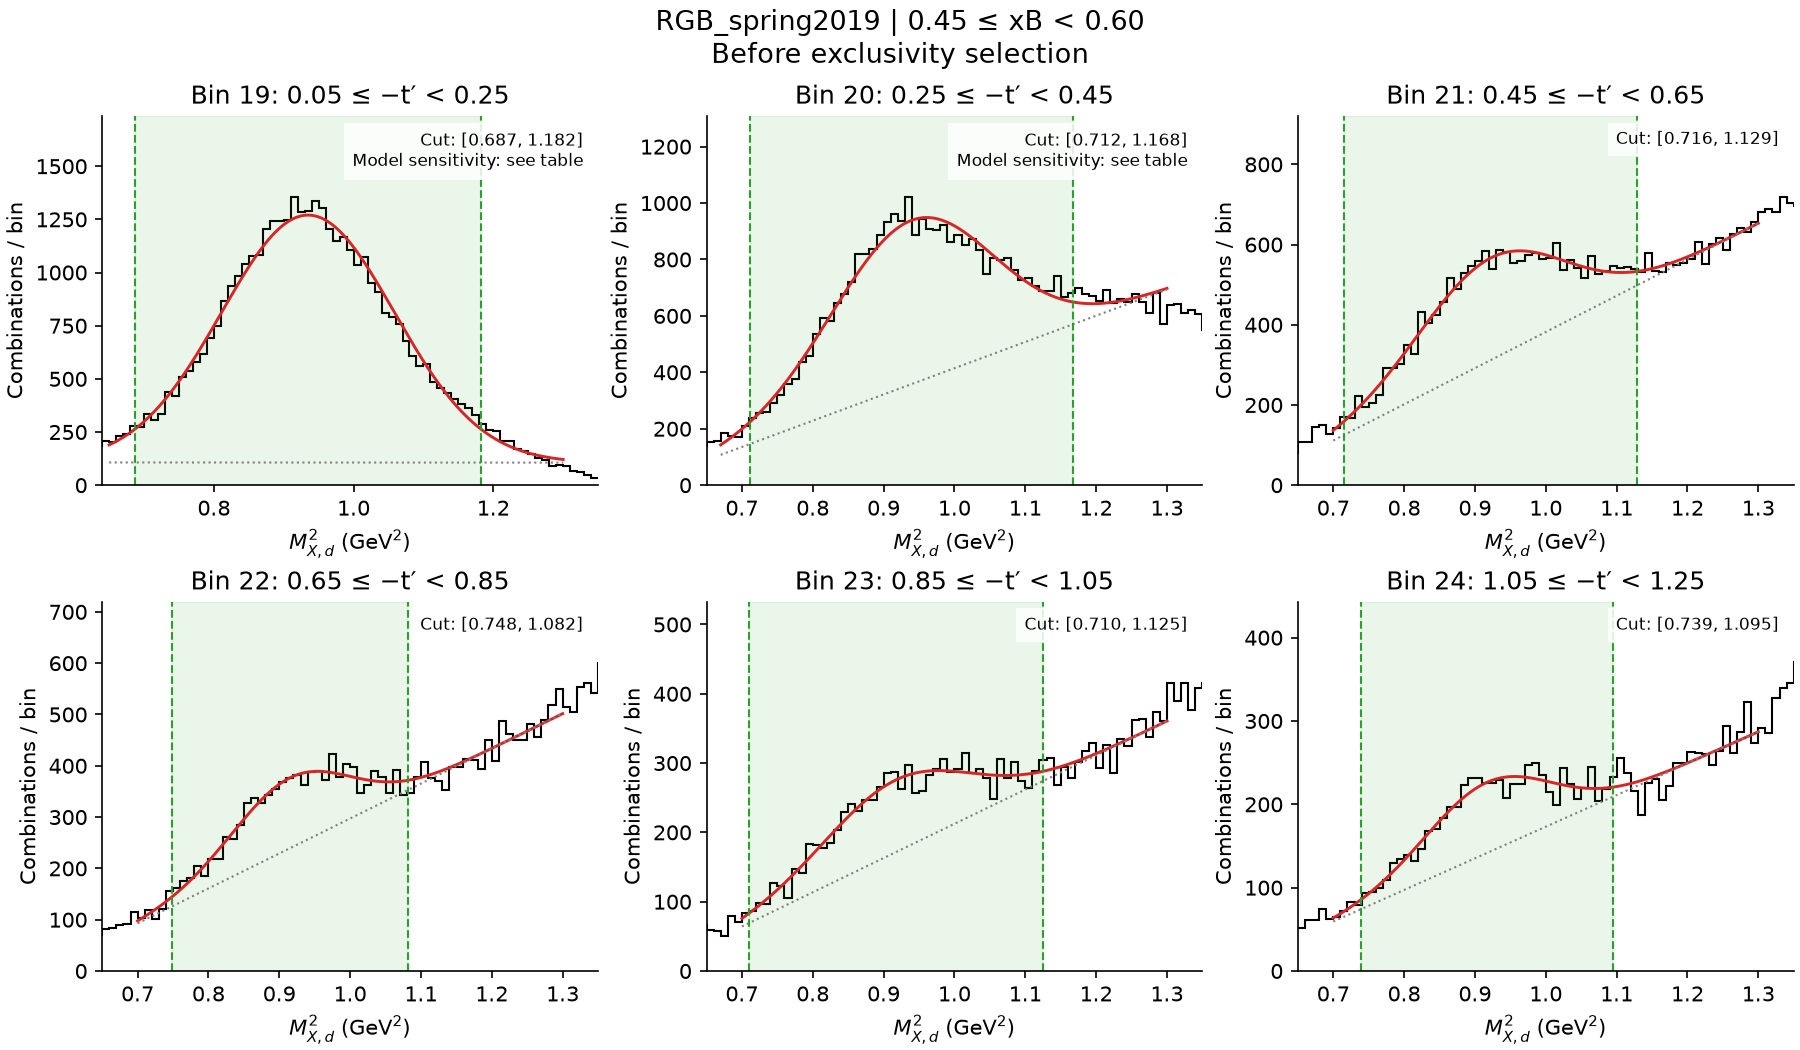
\includegraphics[width=\linewidth]{figures/channel_selection/exclusivity/rgb_sp19_mass_xb4.png}
\caption{RGB\_spring2019: deuteron-reference missing-mass-squared fits in $x_B$ interval 4. The panels retain the six fine selection bins.}\label{fig:new_excl_rgb_sp19_mass4}
\end{figure}
\clearpage
\begin{figure}[p]\centering
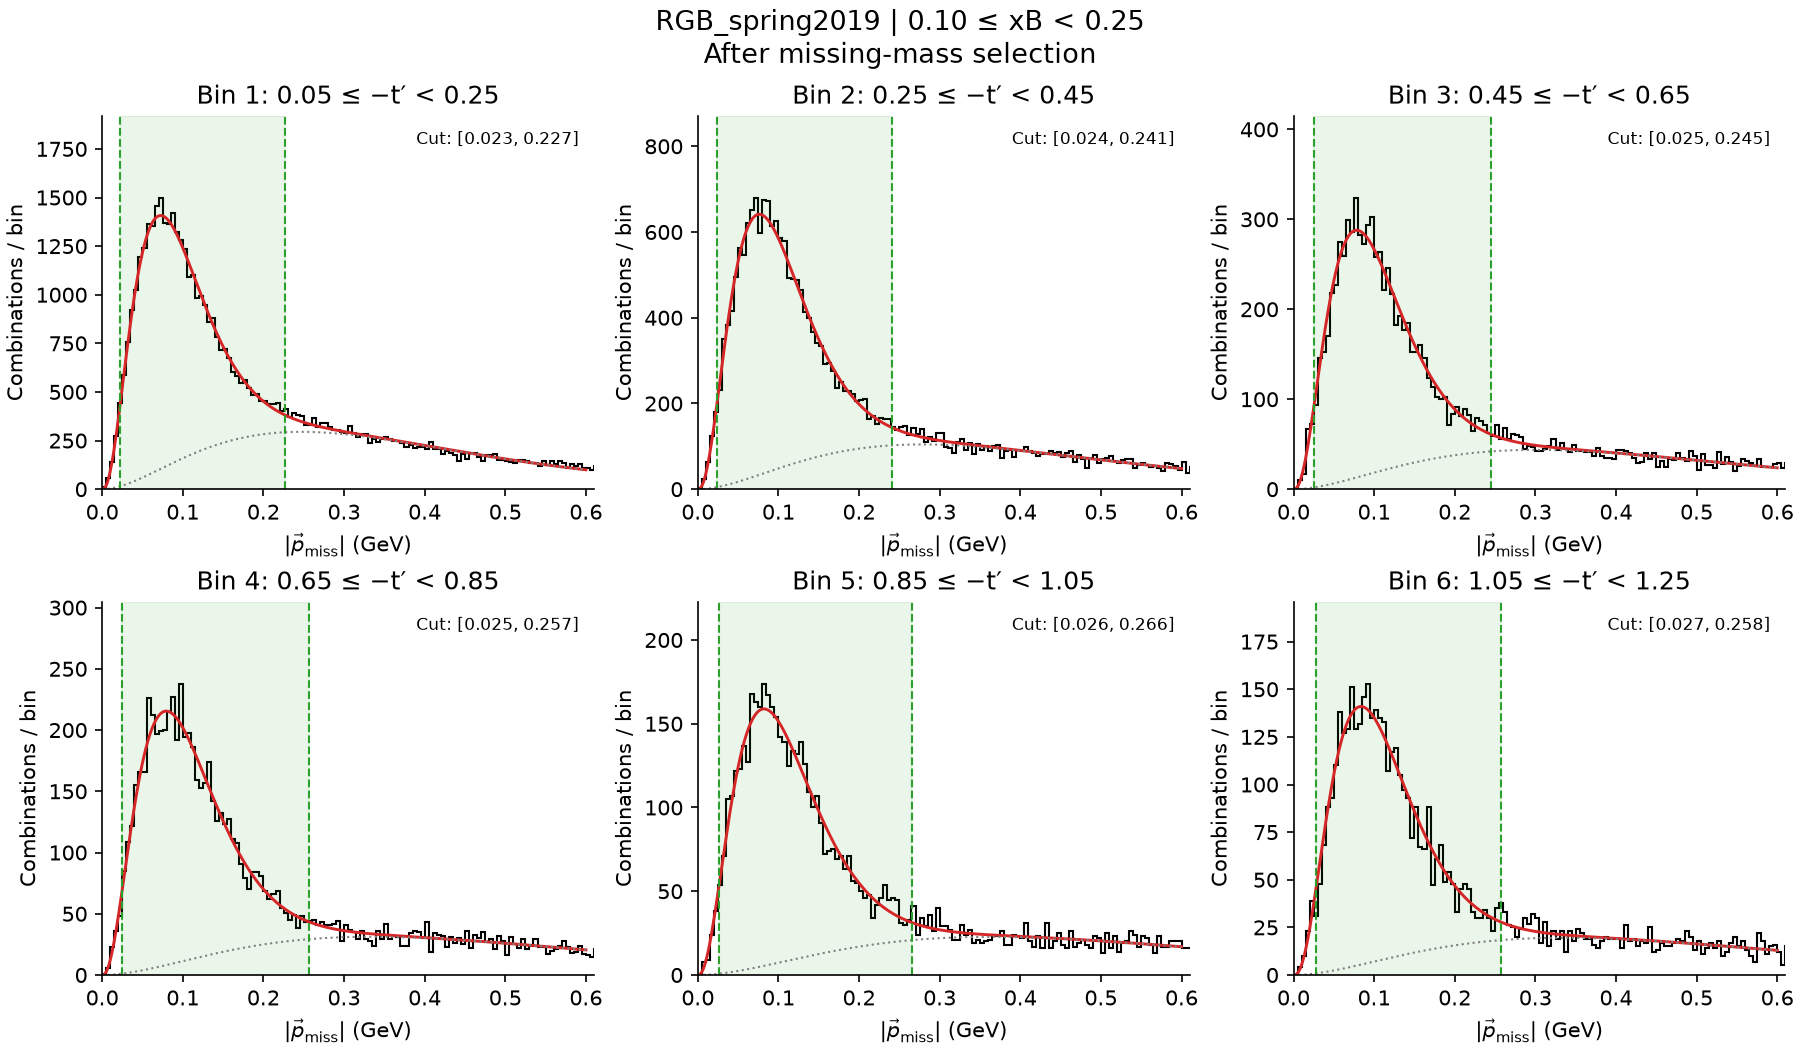
\includegraphics[width=\linewidth]{figures/channel_selection/exclusivity/rgb_sp19_momentum_xb1.png}
\caption{RGB\_spring2019: missing-momentum fits after the mass cut in $x_B$ interval 1. The panels retain the six fine selection bins.}\label{fig:new_excl_rgb_sp19_momentum1}
\end{figure}
\clearpage
\begin{figure}[p]\centering
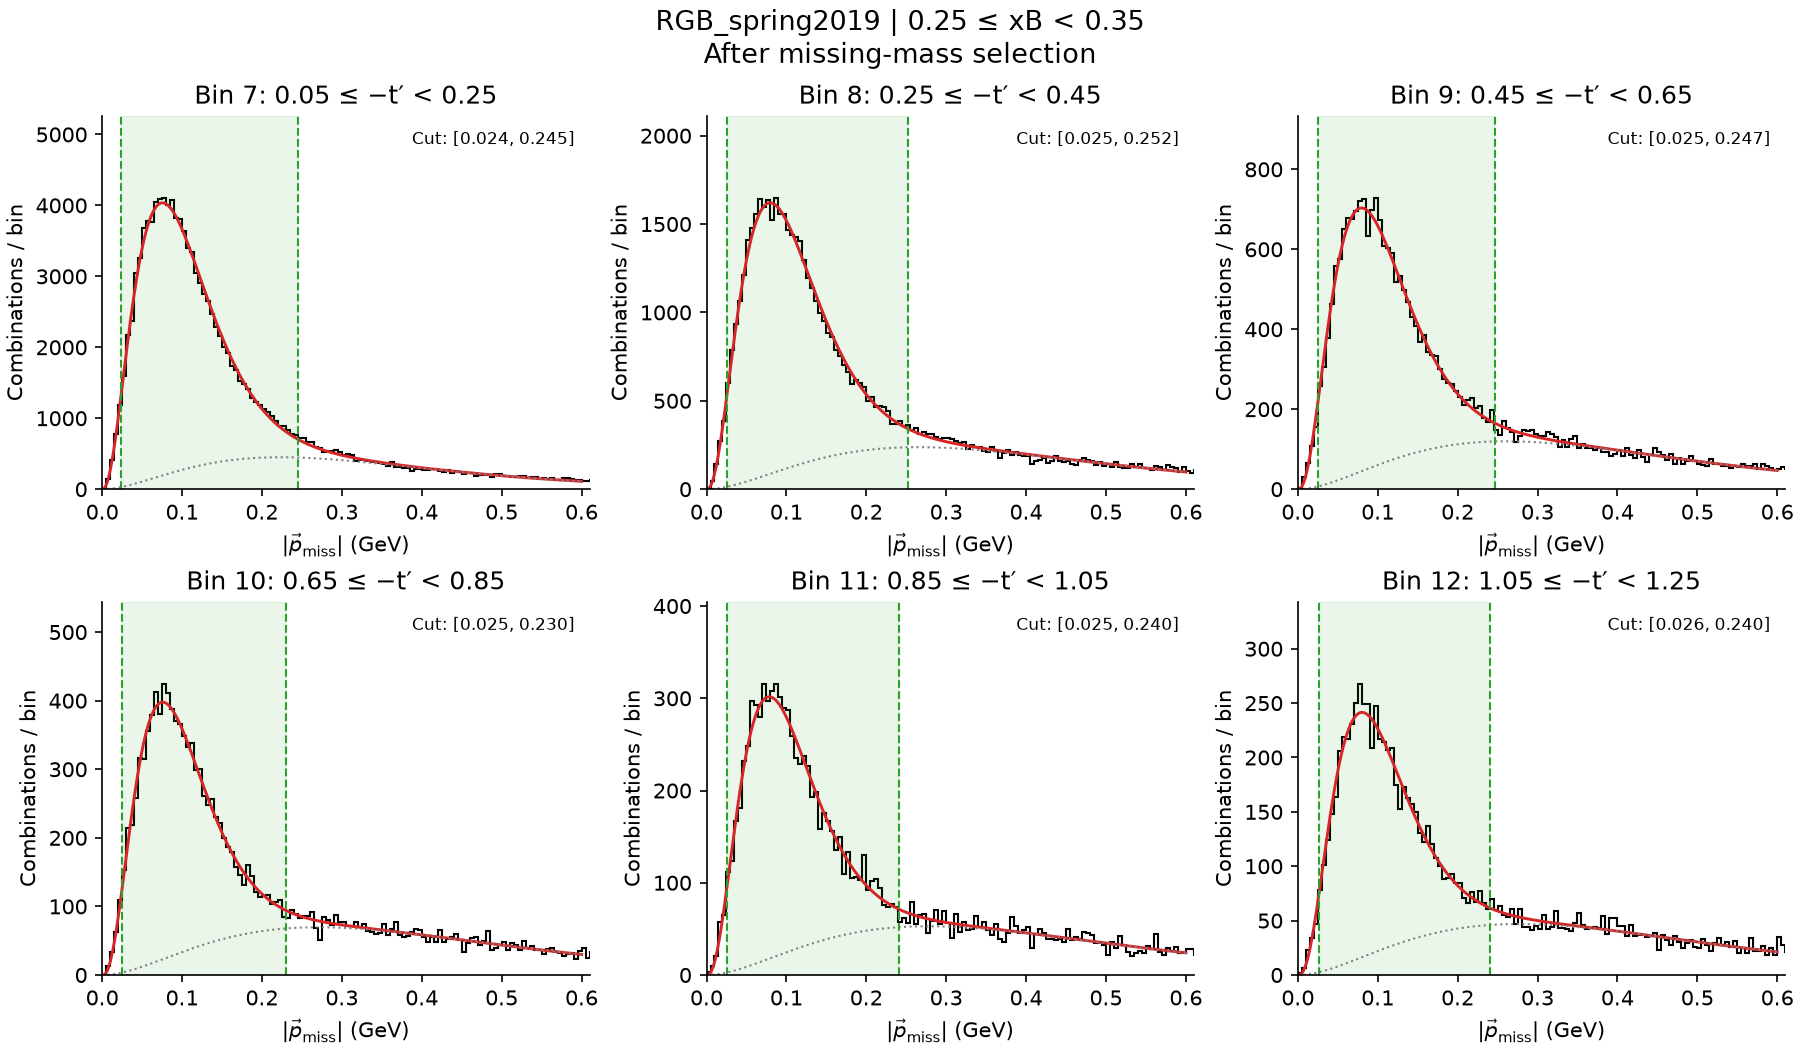
\includegraphics[width=\linewidth]{figures/channel_selection/exclusivity/rgb_sp19_momentum_xb2.png}
\caption{RGB\_spring2019: missing-momentum fits after the mass cut in $x_B$ interval 2. The panels retain the six fine selection bins.}\label{fig:new_excl_rgb_sp19_momentum2}
\end{figure}
\clearpage
\begin{figure}[p]\centering
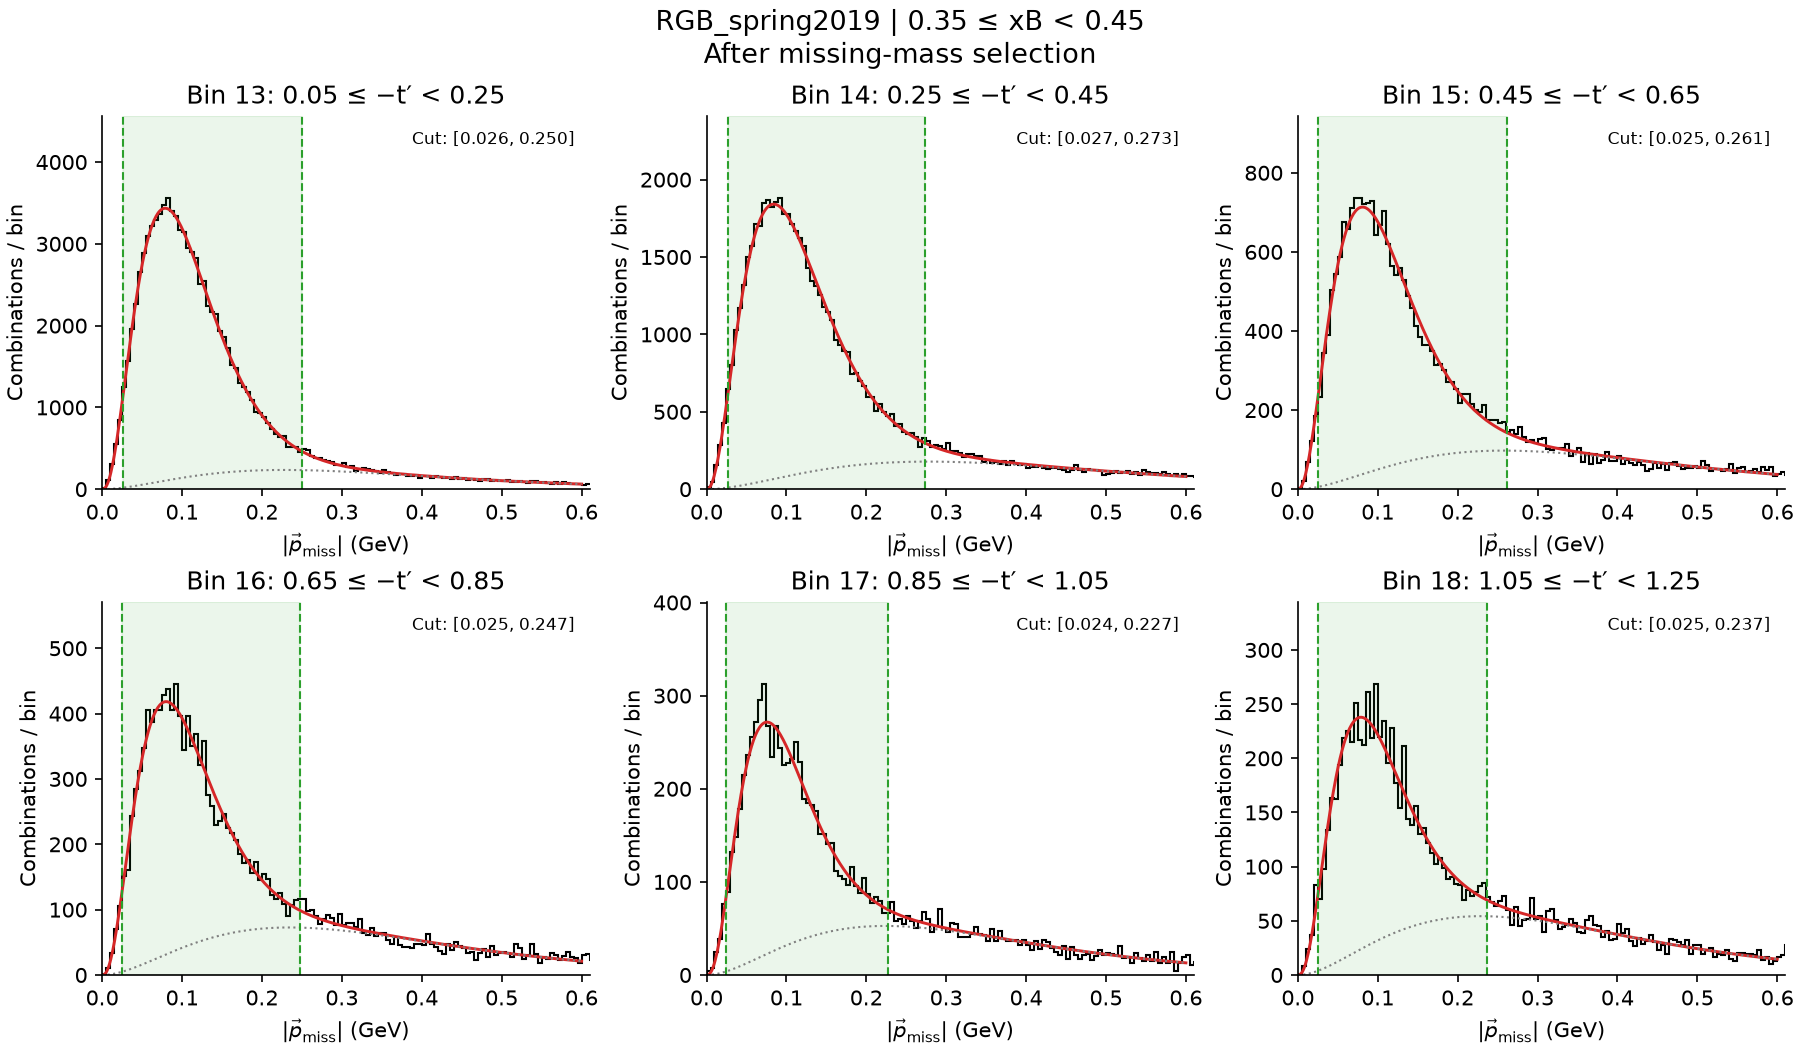
\includegraphics[width=\linewidth]{figures/channel_selection/exclusivity/rgb_sp19_momentum_xb3.png}
\caption{RGB\_spring2019: missing-momentum fits after the mass cut in $x_B$ interval 3. The panels retain the six fine selection bins.}\label{fig:new_excl_rgb_sp19_momentum3}
\end{figure}
\clearpage
\begin{figure}[p]\centering
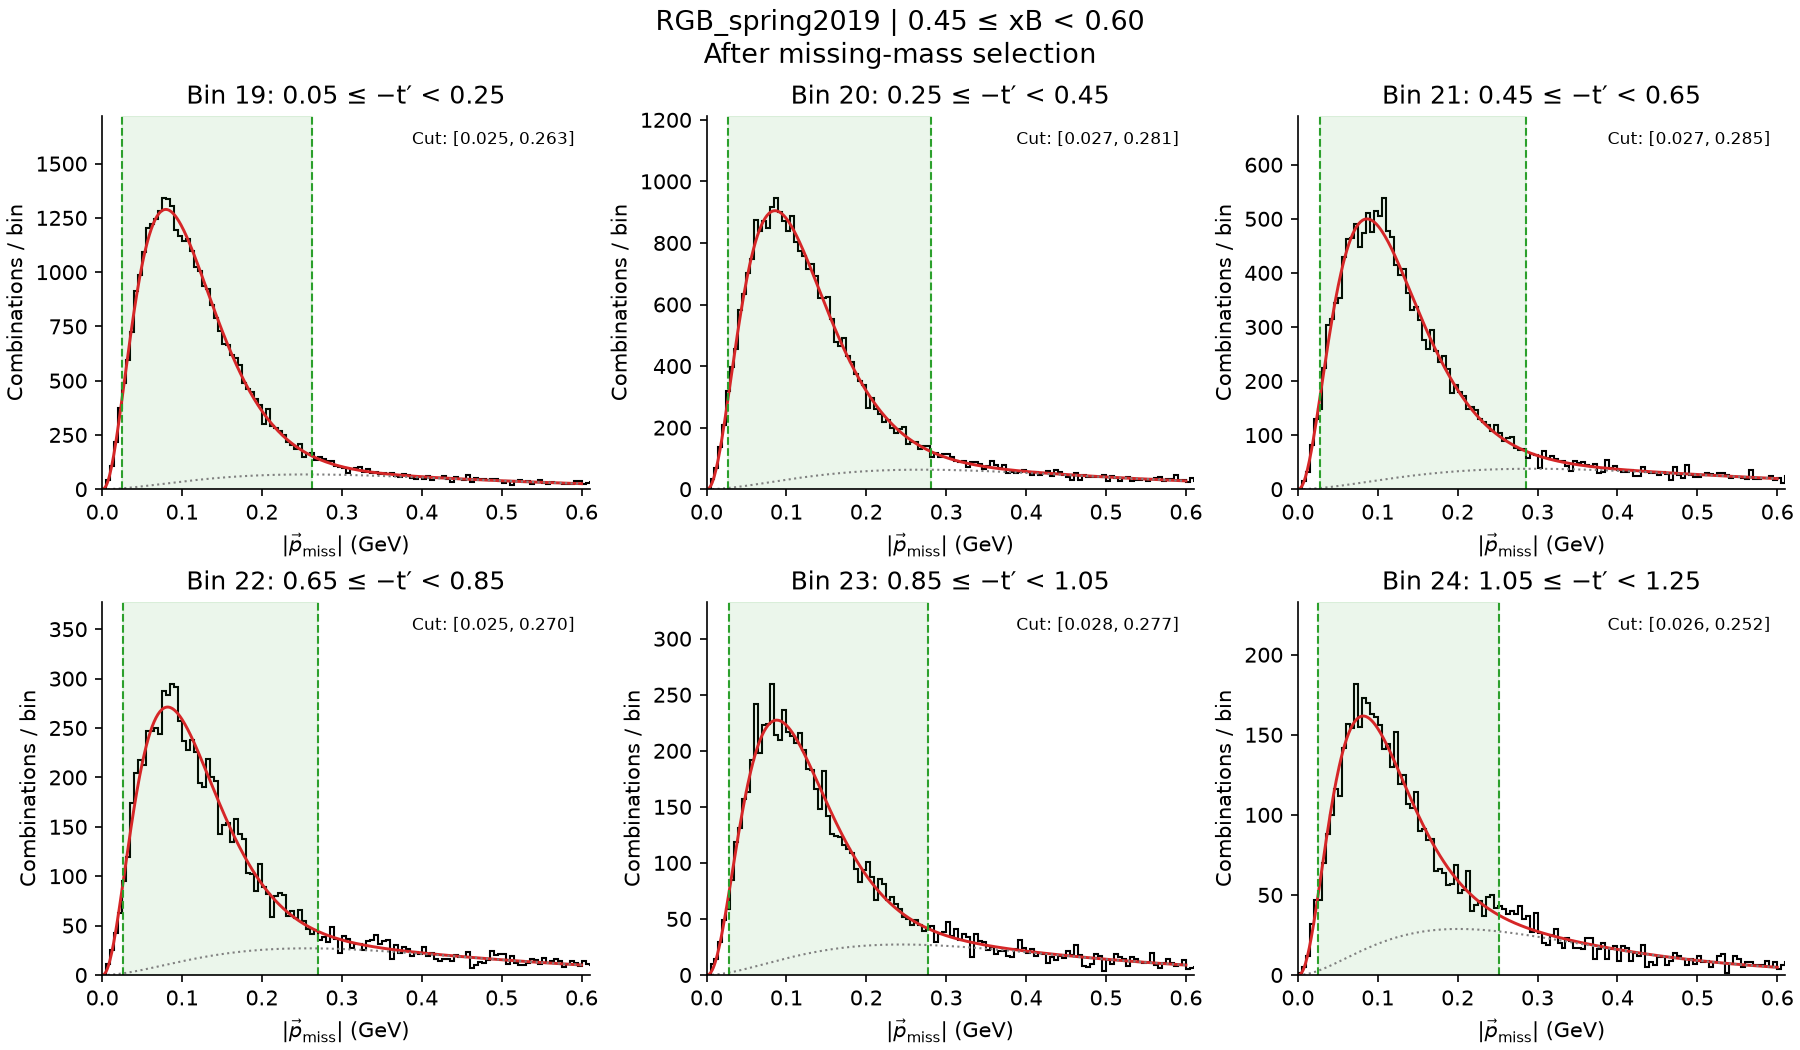
\includegraphics[width=\linewidth]{figures/channel_selection/exclusivity/rgb_sp19_momentum_xb4.png}
\caption{RGB\_spring2019: missing-momentum fits after the mass cut in $x_B$ interval 4. The panels retain the six fine selection bins.}\label{fig:new_excl_rgb_sp19_momentum4}
\end{figure}
\clearpage
\begin{figure}[p]\centering
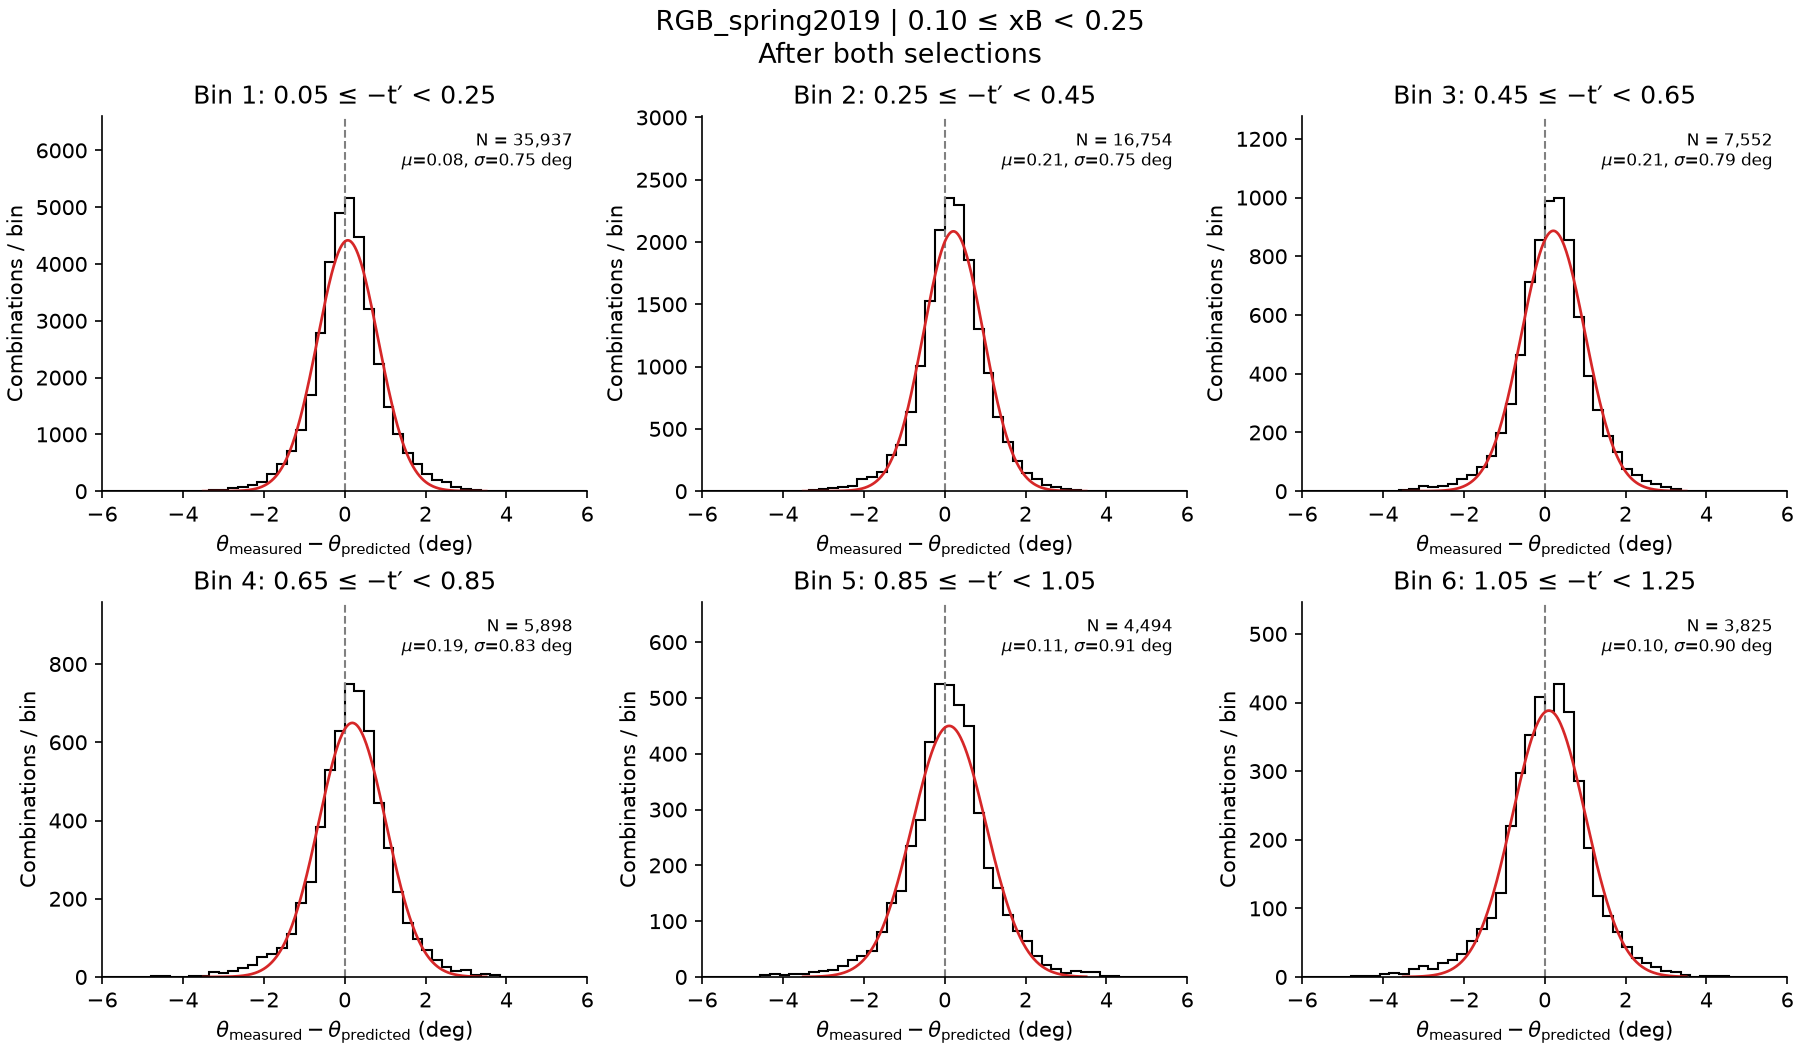
\includegraphics[width=\linewidth]{figures/channel_selection/exclusivity/rgb_sp19_angle_xb1.png}
\caption{RGB\_spring2019: pion polar-angle closure after both cuts in $x_B$ interval 1. The panels retain the six fine selection bins.}\label{fig:new_excl_rgb_sp19_angle1}
\end{figure}
\clearpage
\begin{figure}[p]\centering
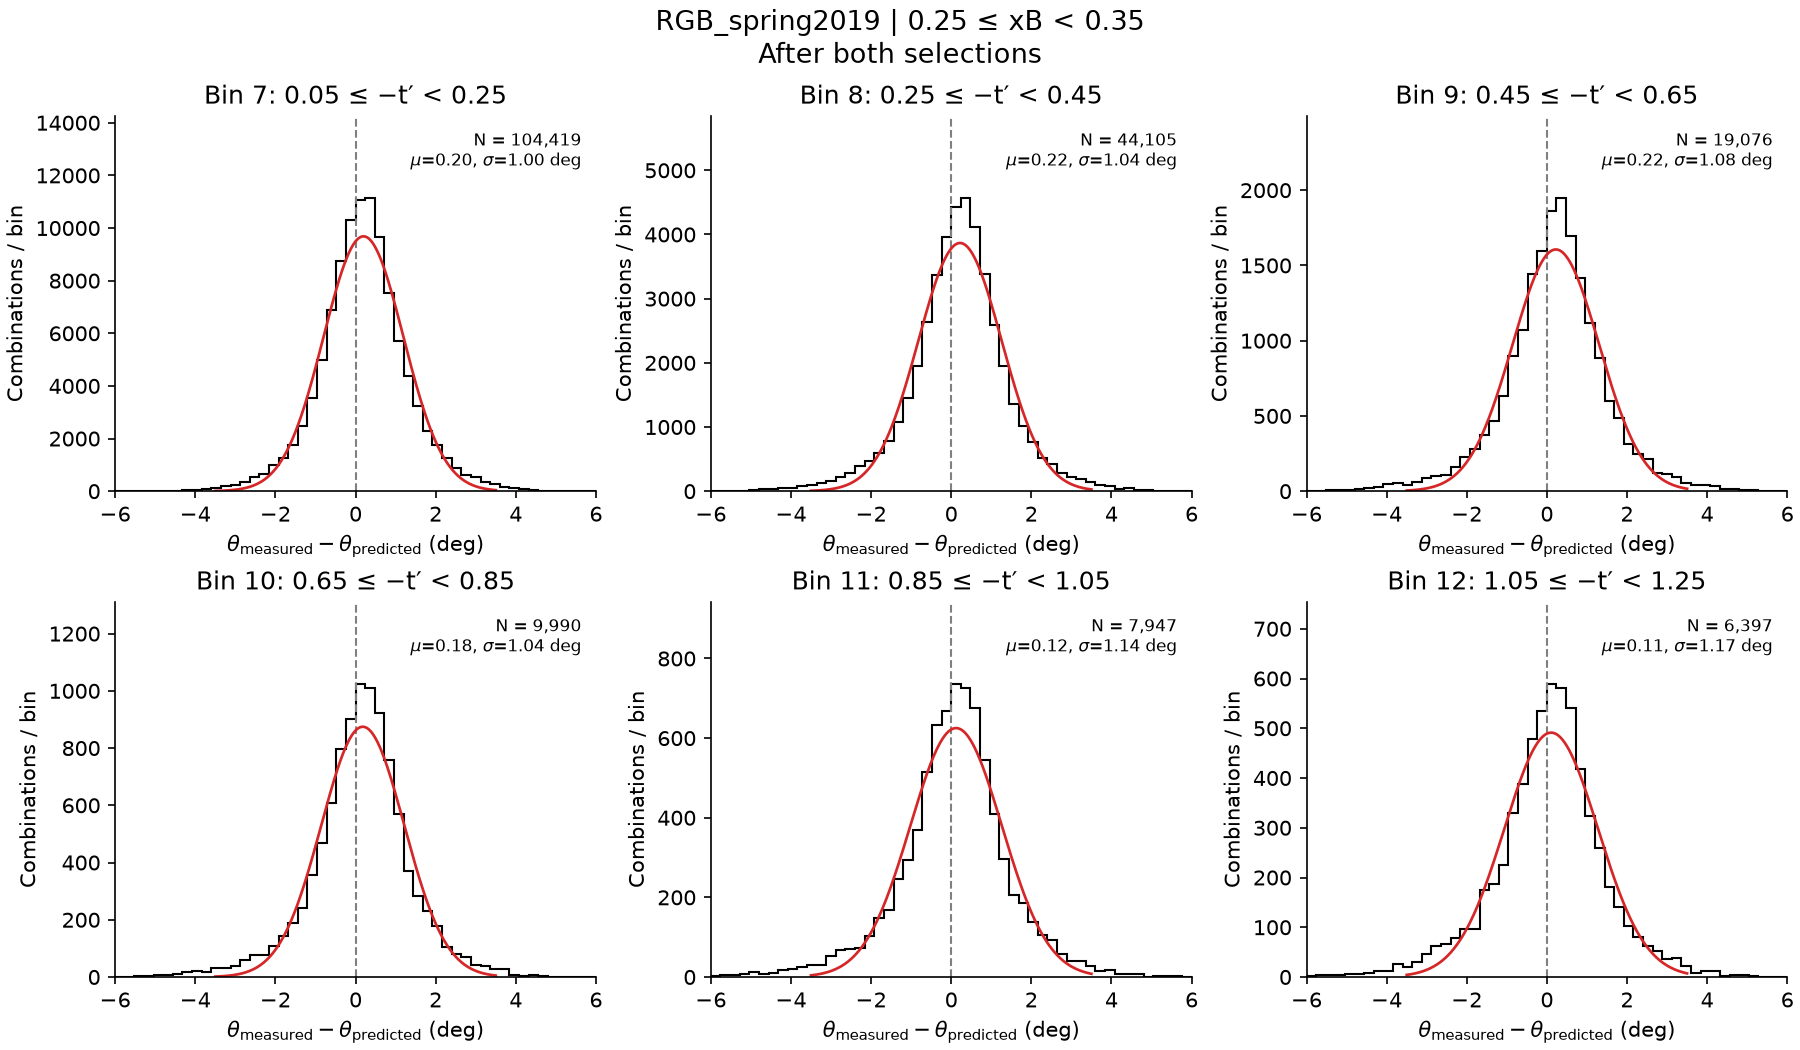
\includegraphics[width=\linewidth]{figures/channel_selection/exclusivity/rgb_sp19_angle_xb2.png}
\caption{RGB\_spring2019: pion polar-angle closure after both cuts in $x_B$ interval 2. The panels retain the six fine selection bins.}\label{fig:new_excl_rgb_sp19_angle2}
\end{figure}
\clearpage
\begin{figure}[p]\centering
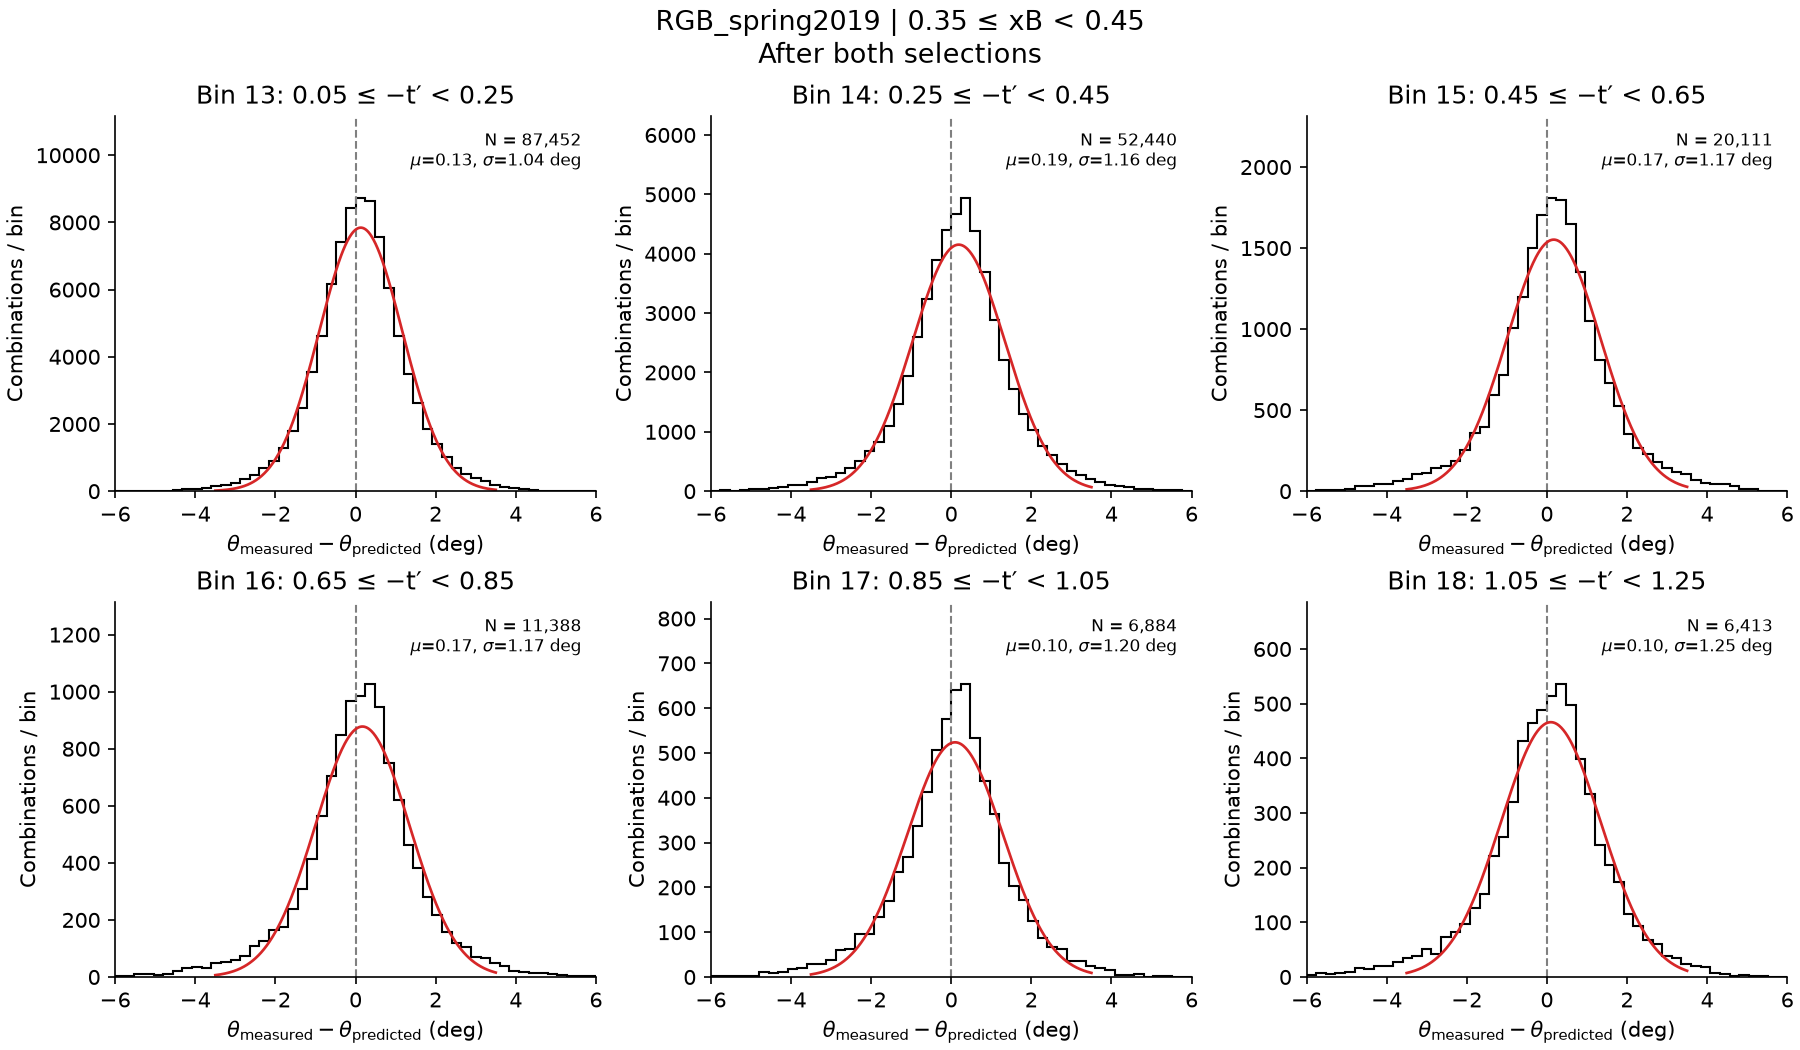
\includegraphics[width=\linewidth]{figures/channel_selection/exclusivity/rgb_sp19_angle_xb3.png}
\caption{RGB\_spring2019: pion polar-angle closure after both cuts in $x_B$ interval 3. The panels retain the six fine selection bins.}\label{fig:new_excl_rgb_sp19_angle3}
\end{figure}
\clearpage
\begin{figure}[p]\centering
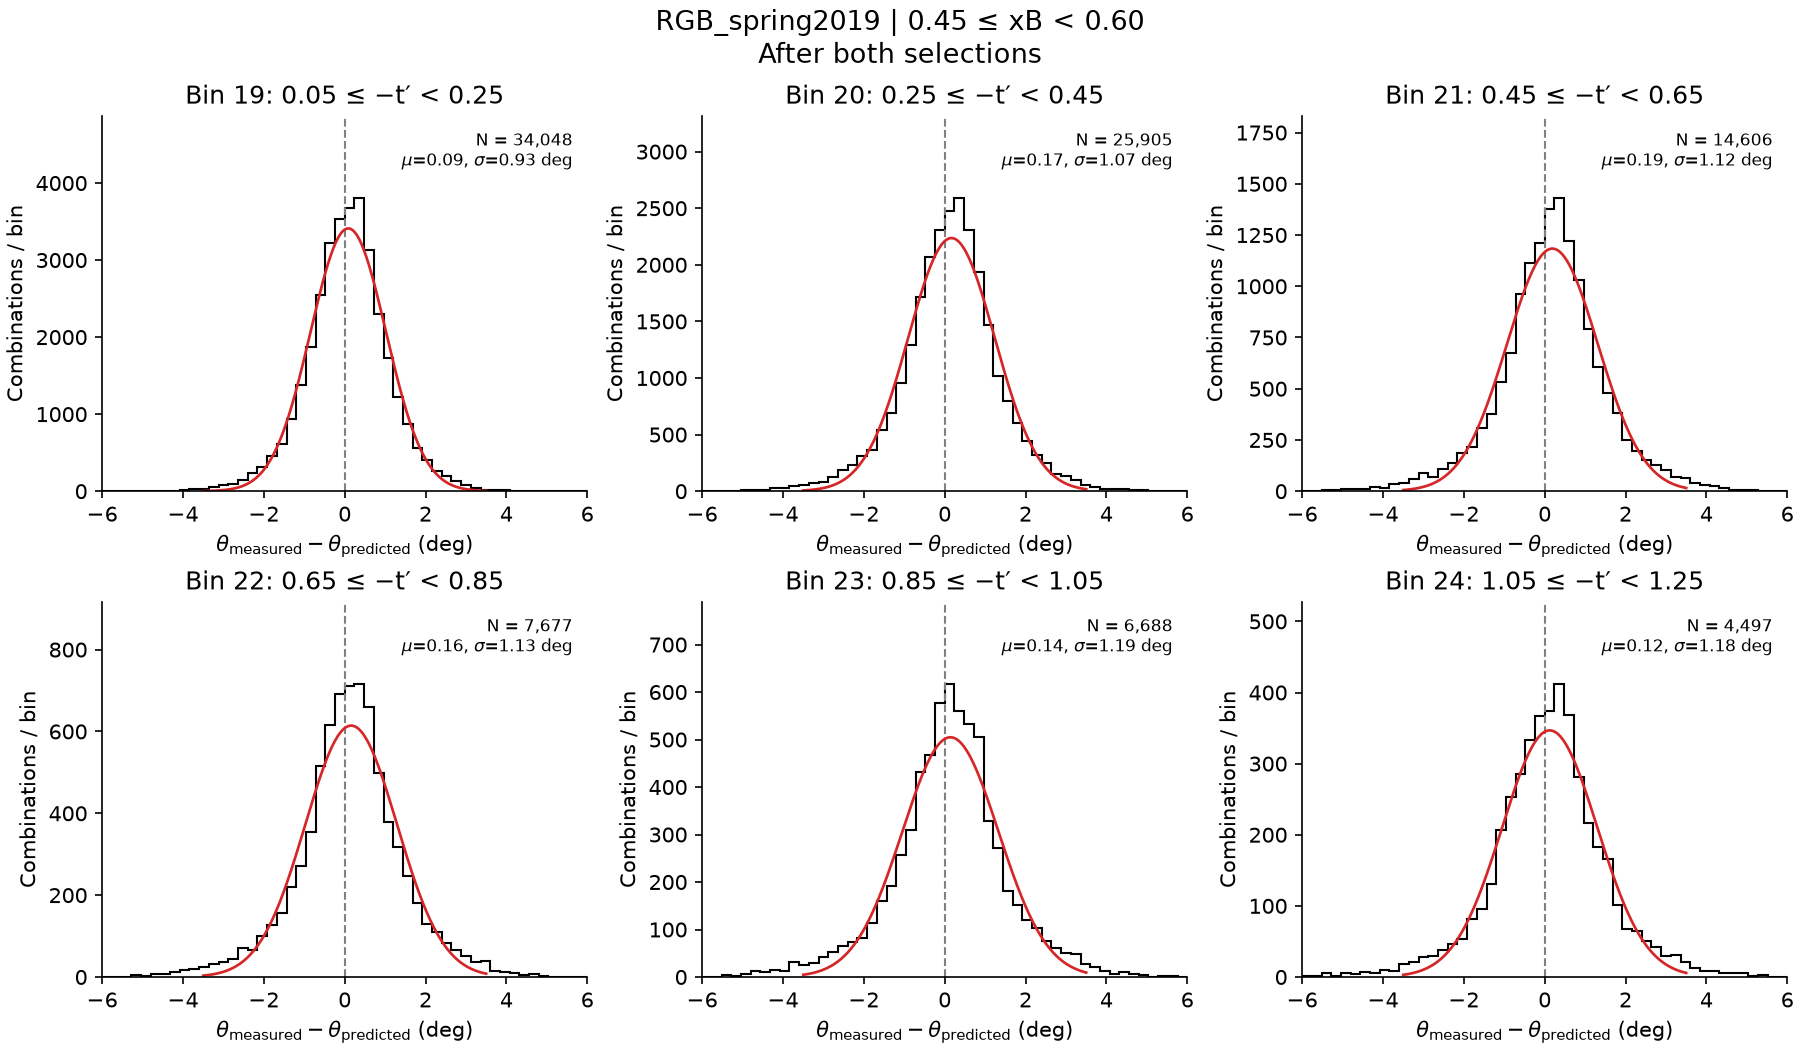
\includegraphics[width=\linewidth]{figures/channel_selection/exclusivity/rgb_sp19_angle_xb4.png}
\caption{RGB\_spring2019: pion polar-angle closure after both cuts in $x_B$ interval 4. The panels retain the six fine selection bins.}\label{fig:new_excl_rgb_sp19_angle4}
\end{figure}
\clearpage
\begin{figure}[p]\centering
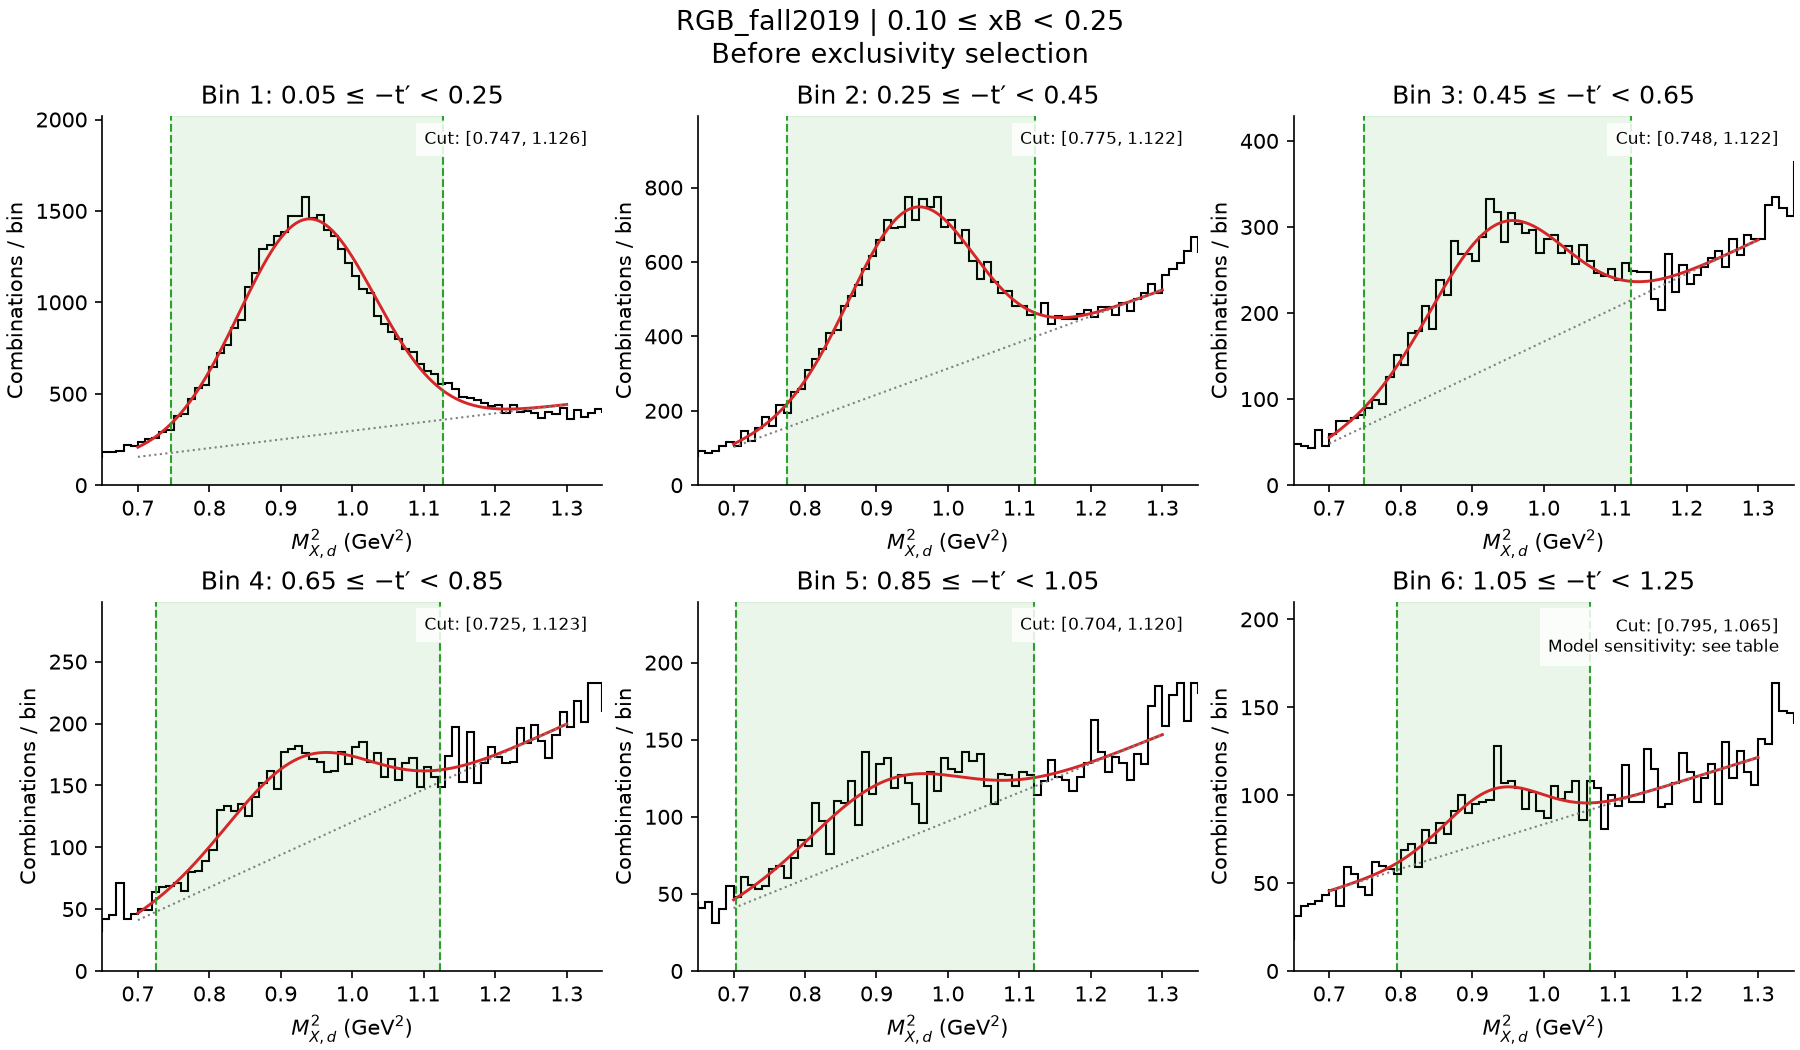
\includegraphics[width=\linewidth]{figures/channel_selection/exclusivity/rgb_fa19_mass_xb1.png}
\caption{RGB\_fall2019: deuteron-reference missing-mass-squared fits in $x_B$ interval 1. The panels retain the six fine selection bins.}\label{fig:new_excl_rgb_fa19_mass1}
\end{figure}
\clearpage
\begin{figure}[p]\centering
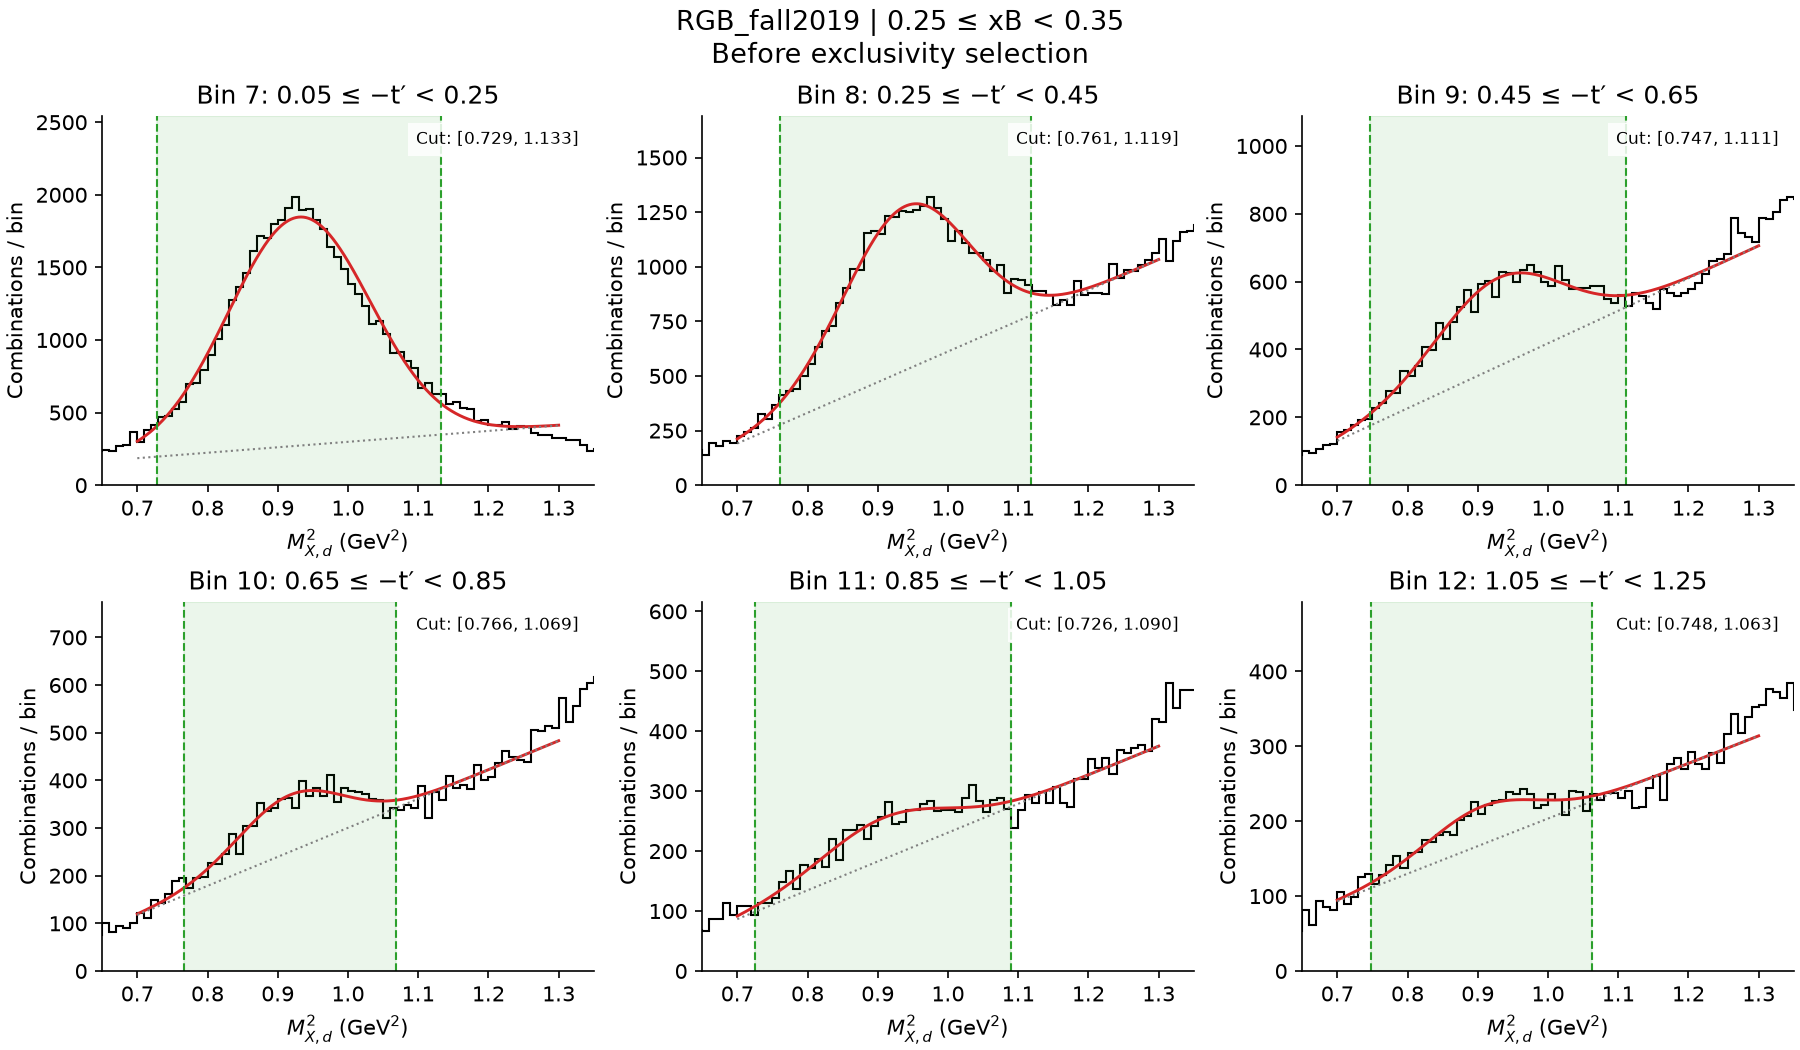
\includegraphics[width=\linewidth]{figures/channel_selection/exclusivity/rgb_fa19_mass_xb2.png}
\caption{RGB\_fall2019: deuteron-reference missing-mass-squared fits in $x_B$ interval 2. The panels retain the six fine selection bins.}\label{fig:new_excl_rgb_fa19_mass2}
\end{figure}
\clearpage
\begin{figure}[p]\centering
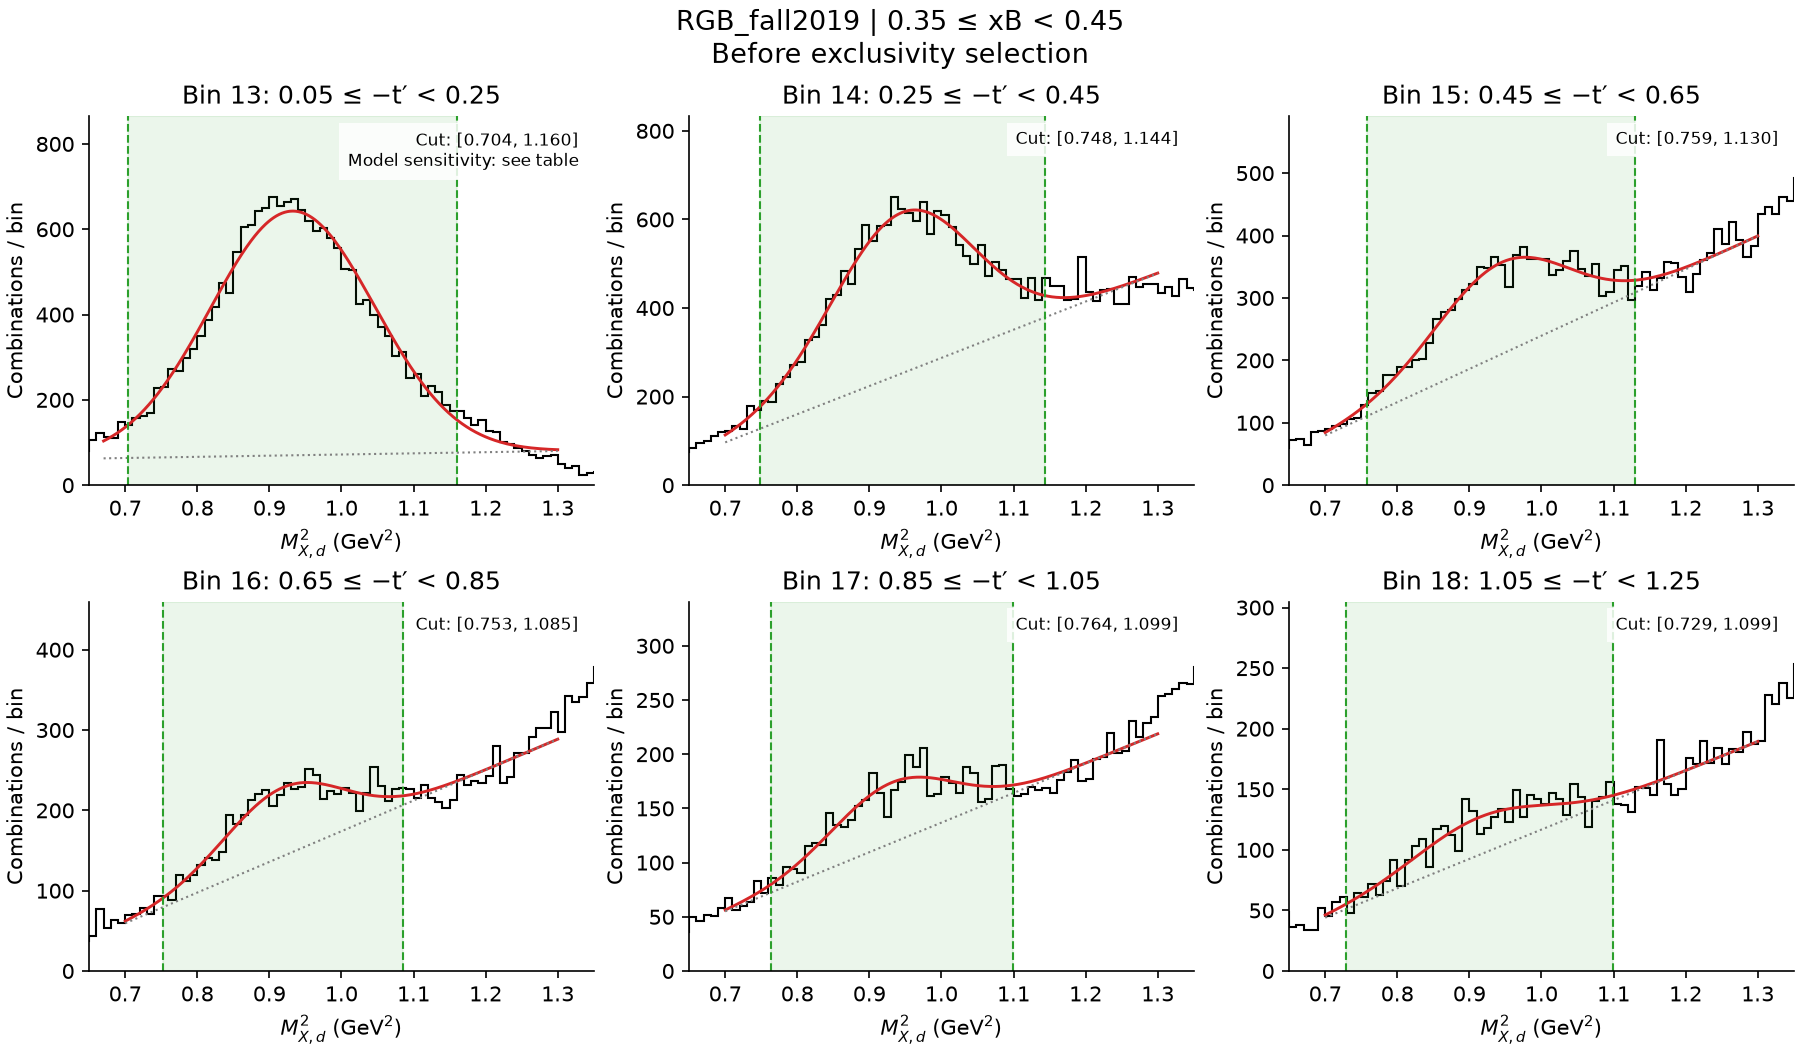
\includegraphics[width=\linewidth]{figures/channel_selection/exclusivity/rgb_fa19_mass_xb3.png}
\caption{RGB\_fall2019: deuteron-reference missing-mass-squared fits in $x_B$ interval 3. The panels retain the six fine selection bins.}\label{fig:new_excl_rgb_fa19_mass3}
\end{figure}
\clearpage
\begin{figure}[p]\centering
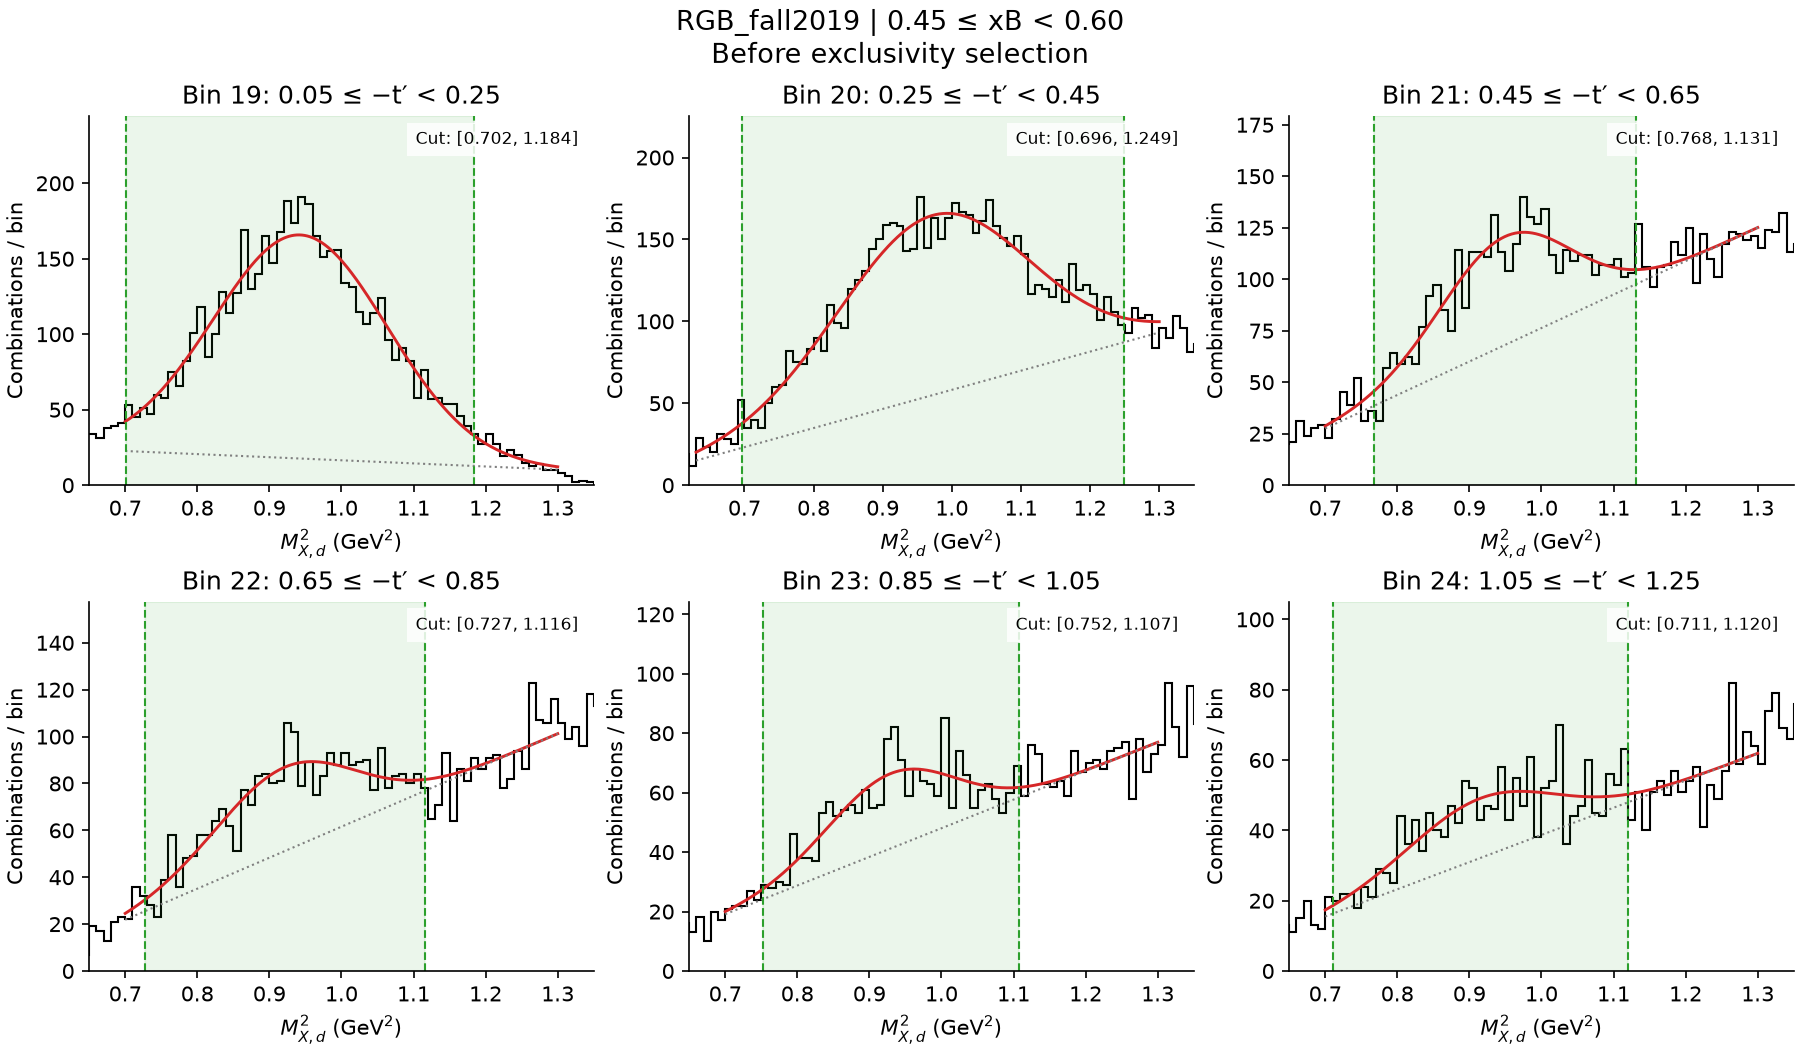
\includegraphics[width=\linewidth]{figures/channel_selection/exclusivity/rgb_fa19_mass_xb4.png}
\caption{RGB\_fall2019: deuteron-reference missing-mass-squared fits in $x_B$ interval 4. The panels retain the six fine selection bins.}\label{fig:new_excl_rgb_fa19_mass4}
\end{figure}
\clearpage
\begin{figure}[p]\centering
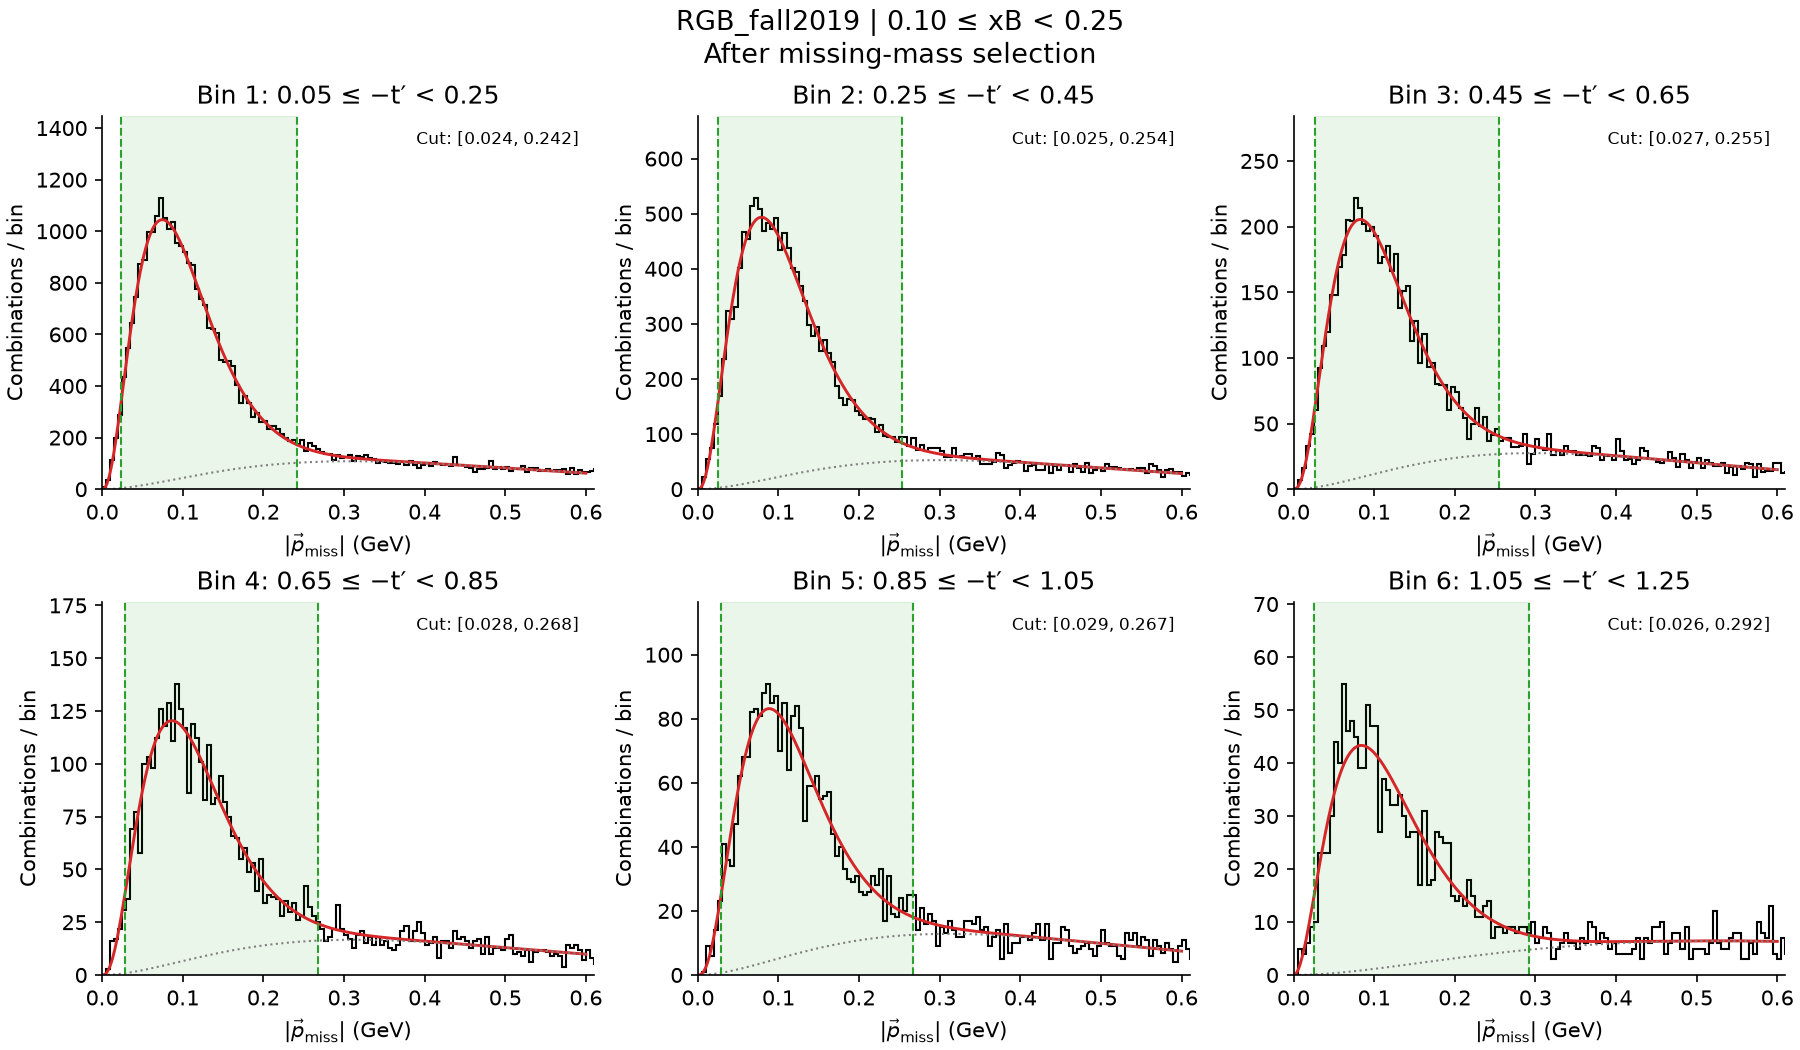
\includegraphics[width=\linewidth]{figures/channel_selection/exclusivity/rgb_fa19_momentum_xb1.png}
\caption{RGB\_fall2019: missing-momentum fits after the mass cut in $x_B$ interval 1. The panels retain the six fine selection bins.}\label{fig:new_excl_rgb_fa19_momentum1}
\end{figure}
\clearpage
\begin{figure}[p]\centering
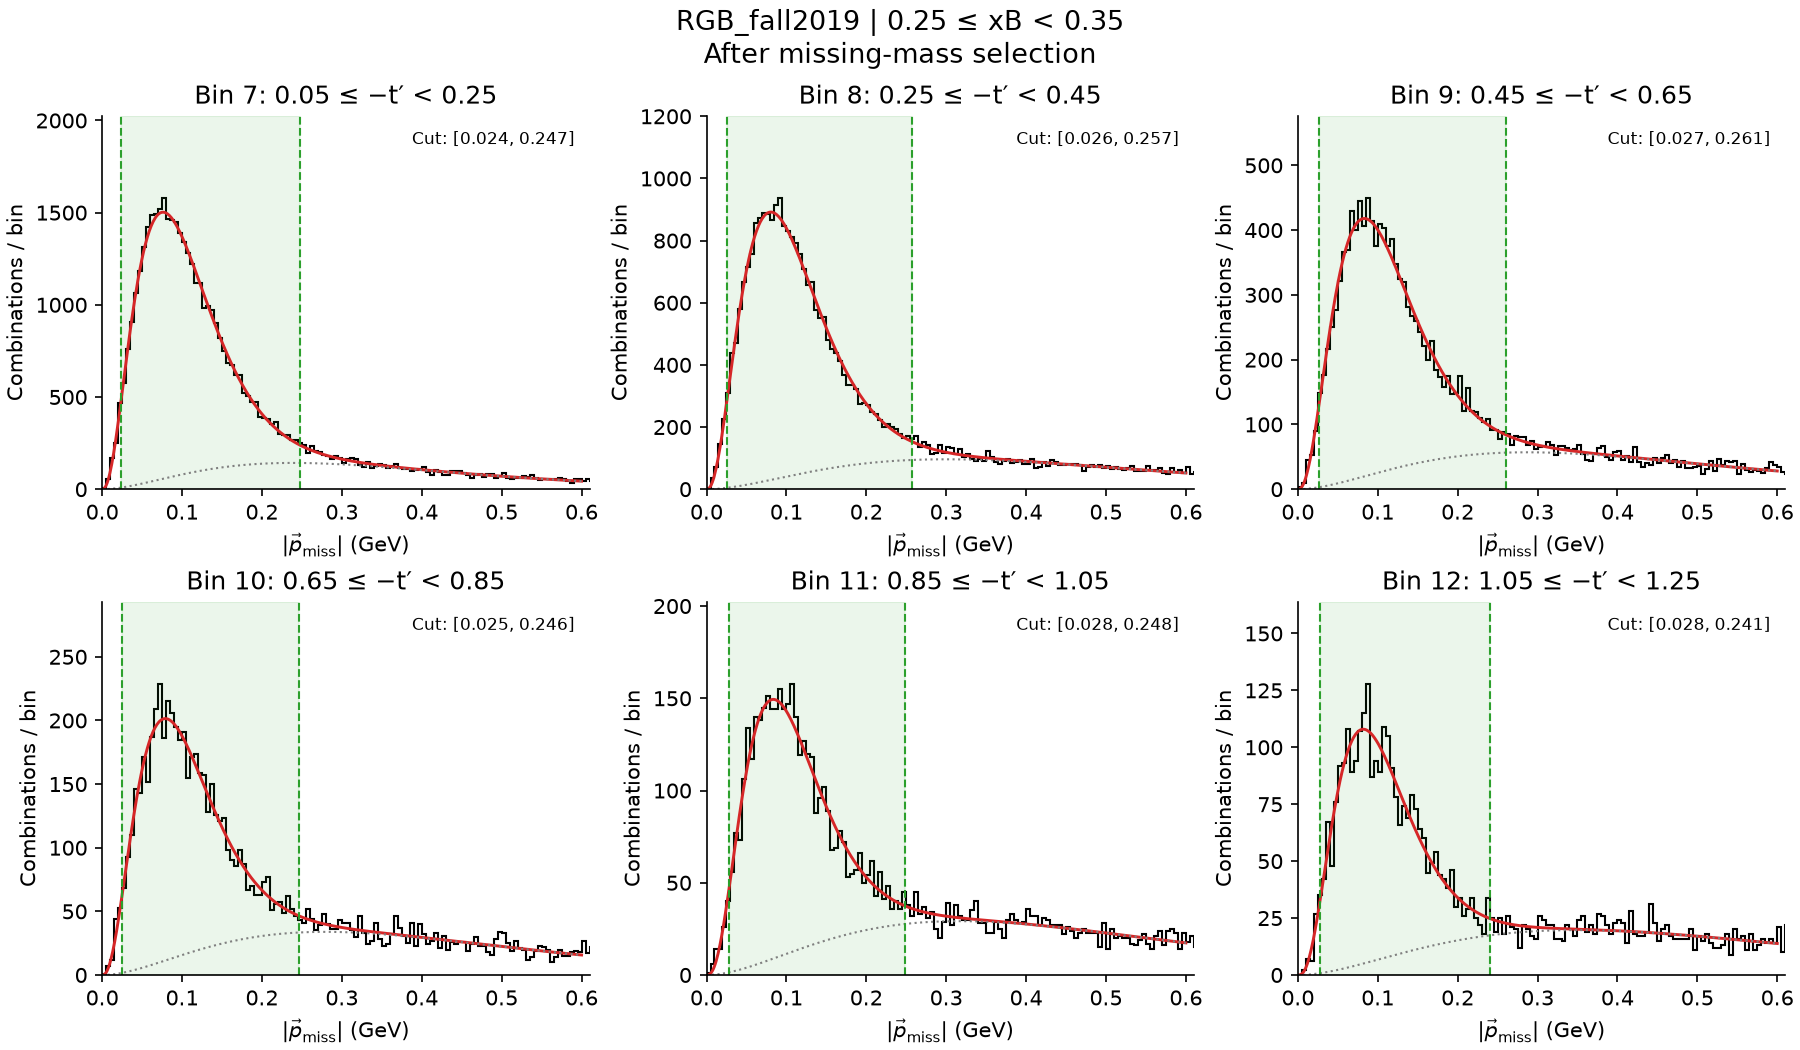
\includegraphics[width=\linewidth]{figures/channel_selection/exclusivity/rgb_fa19_momentum_xb2.png}
\caption{RGB\_fall2019: missing-momentum fits after the mass cut in $x_B$ interval 2. The panels retain the six fine selection bins.}\label{fig:new_excl_rgb_fa19_momentum2}
\end{figure}
\clearpage
\begin{figure}[p]\centering
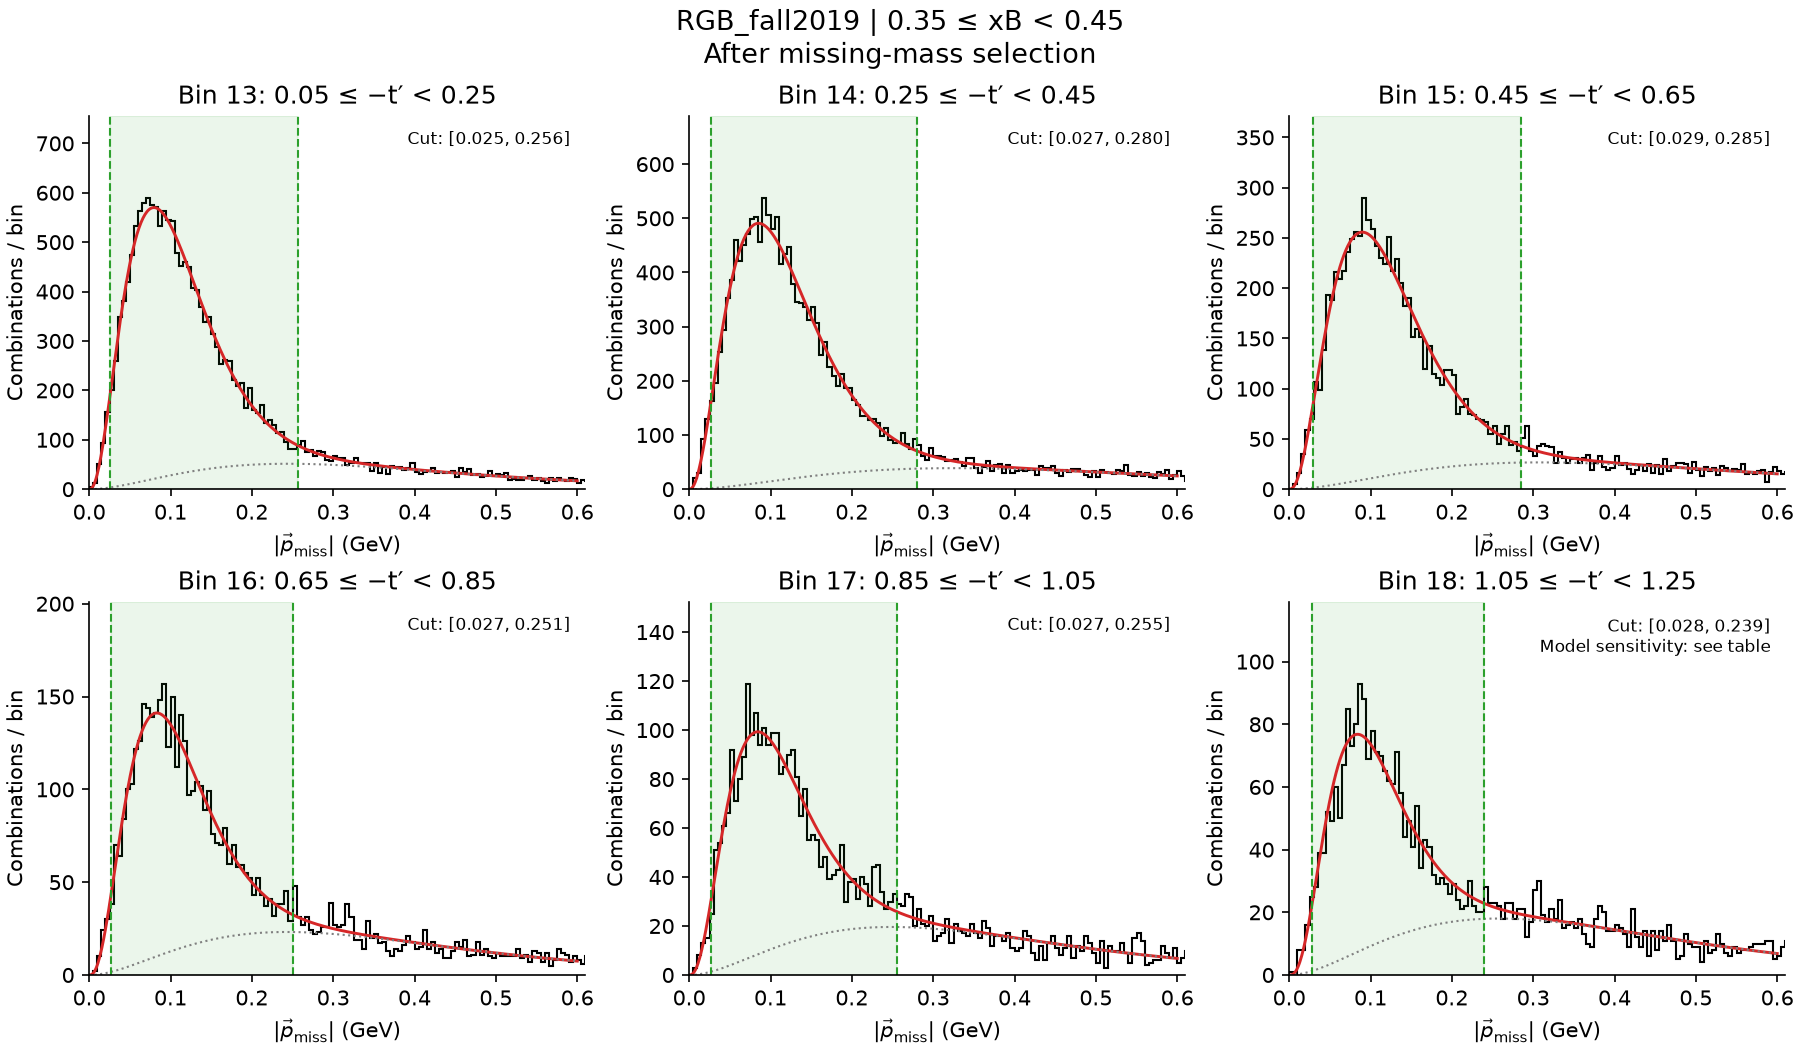
\includegraphics[width=\linewidth]{figures/channel_selection/exclusivity/rgb_fa19_momentum_xb3.png}
\caption{RGB\_fall2019: missing-momentum fits after the mass cut in $x_B$ interval 3. The panels retain the six fine selection bins.}\label{fig:new_excl_rgb_fa19_momentum3}
\end{figure}
\clearpage
\begin{figure}[p]\centering
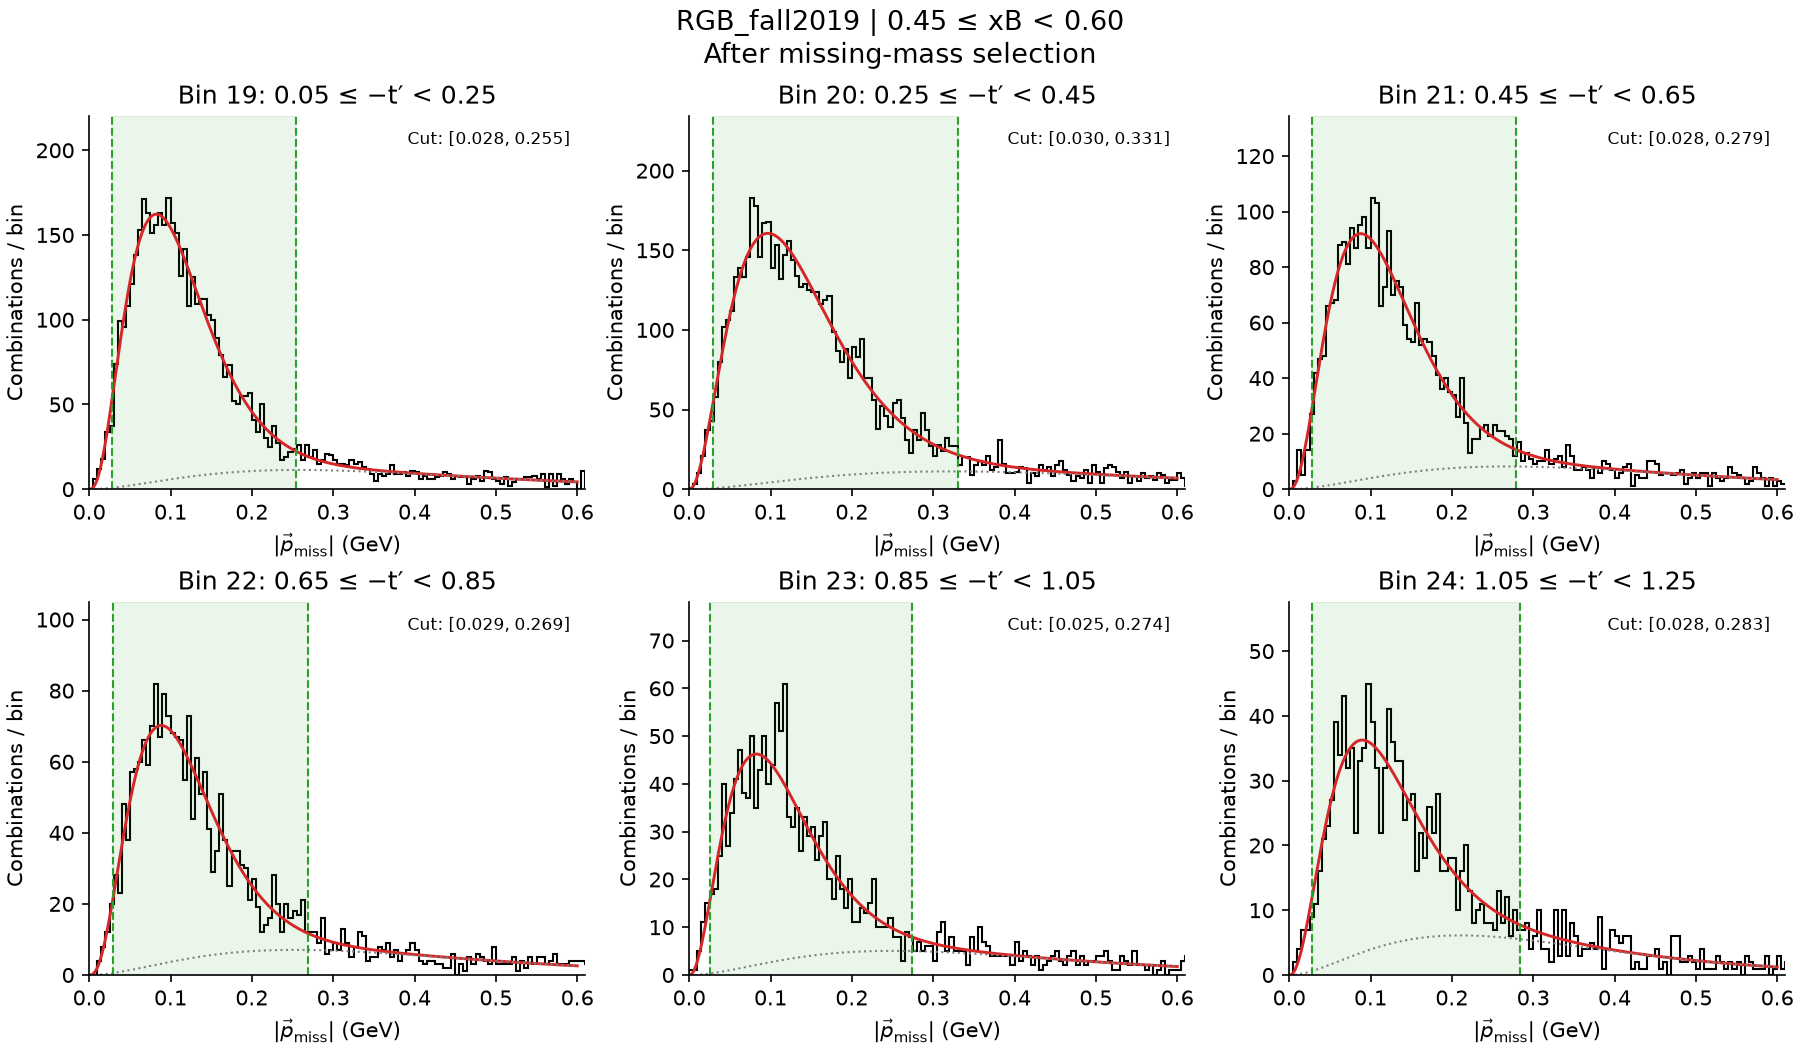
\includegraphics[width=\linewidth]{figures/channel_selection/exclusivity/rgb_fa19_momentum_xb4.png}
\caption{RGB\_fall2019: missing-momentum fits after the mass cut in $x_B$ interval 4. The panels retain the six fine selection bins.}\label{fig:new_excl_rgb_fa19_momentum4}
\end{figure}
\clearpage
\begin{figure}[p]\centering
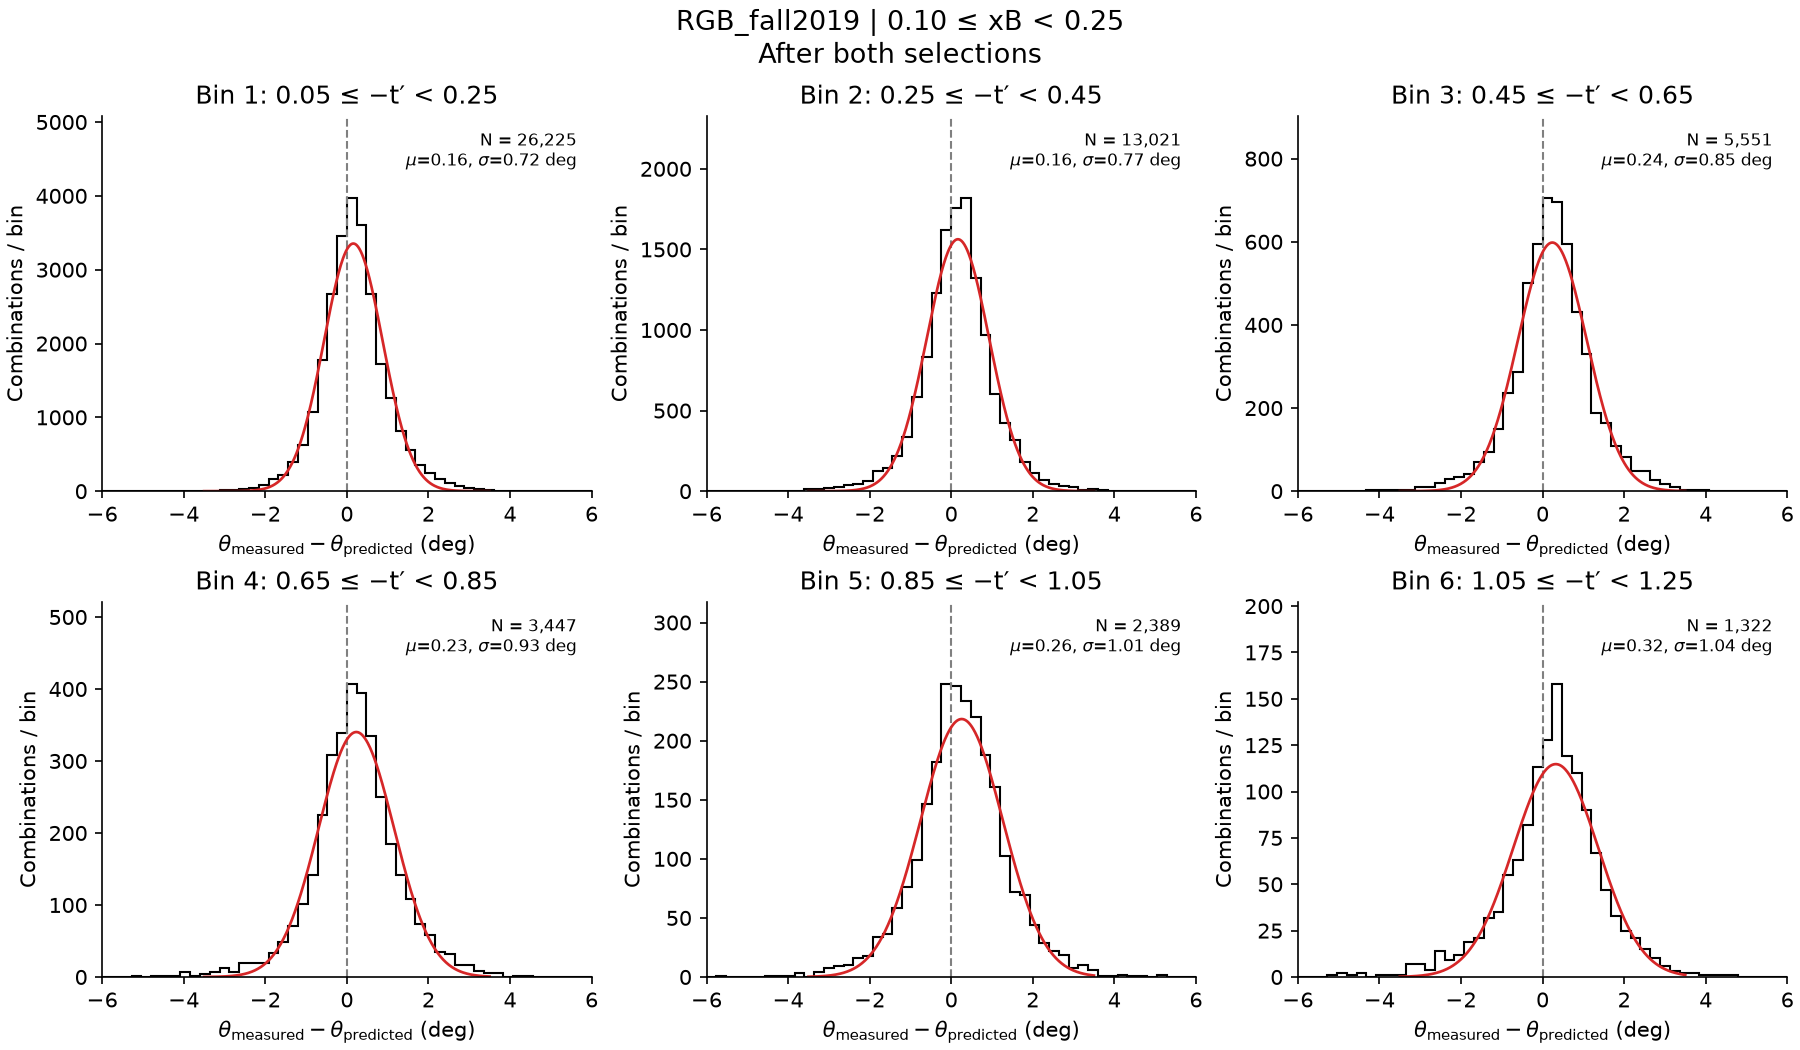
\includegraphics[width=\linewidth]{figures/channel_selection/exclusivity/rgb_fa19_angle_xb1.png}
\caption{RGB\_fall2019: pion polar-angle closure after both cuts in $x_B$ interval 1. The panels retain the six fine selection bins.}\label{fig:new_excl_rgb_fa19_angle1}
\end{figure}
\clearpage
\begin{figure}[p]\centering
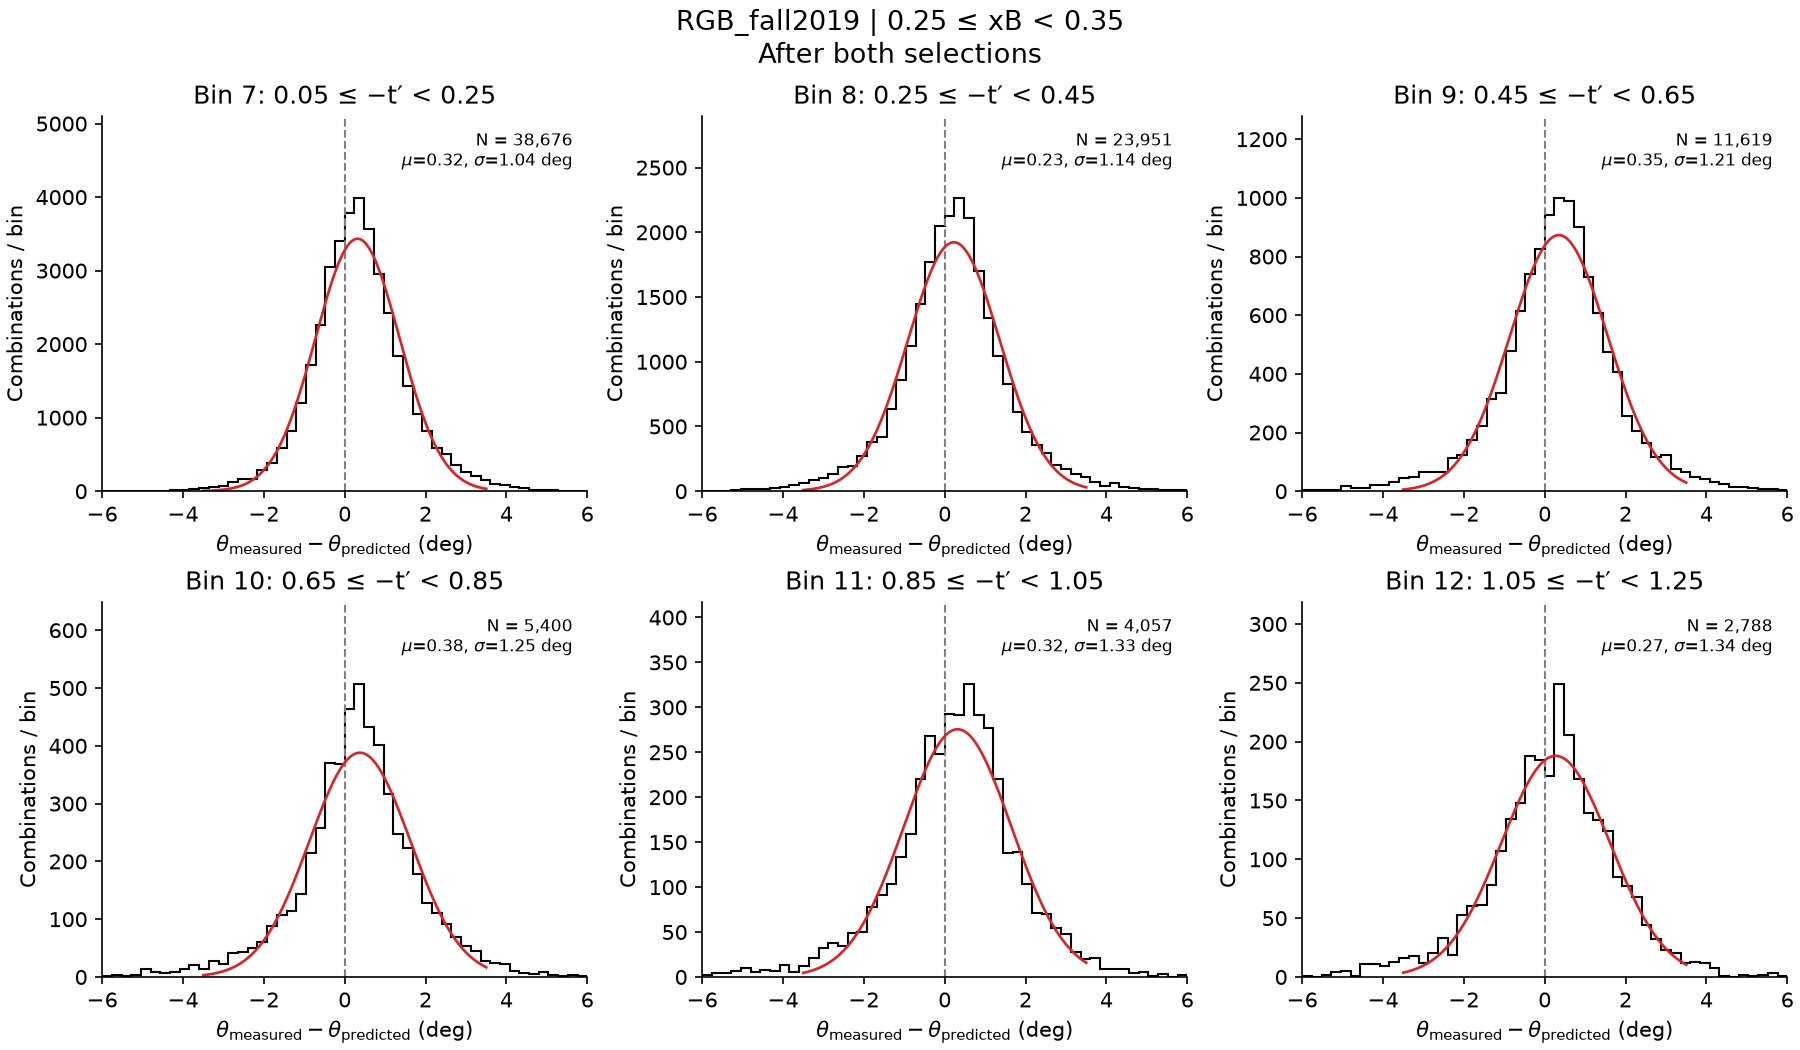
\includegraphics[width=\linewidth]{figures/channel_selection/exclusivity/rgb_fa19_angle_xb2.png}
\caption{RGB\_fall2019: pion polar-angle closure after both cuts in $x_B$ interval 2. The panels retain the six fine selection bins.}\label{fig:new_excl_rgb_fa19_angle2}
\end{figure}
\clearpage
\begin{figure}[p]\centering
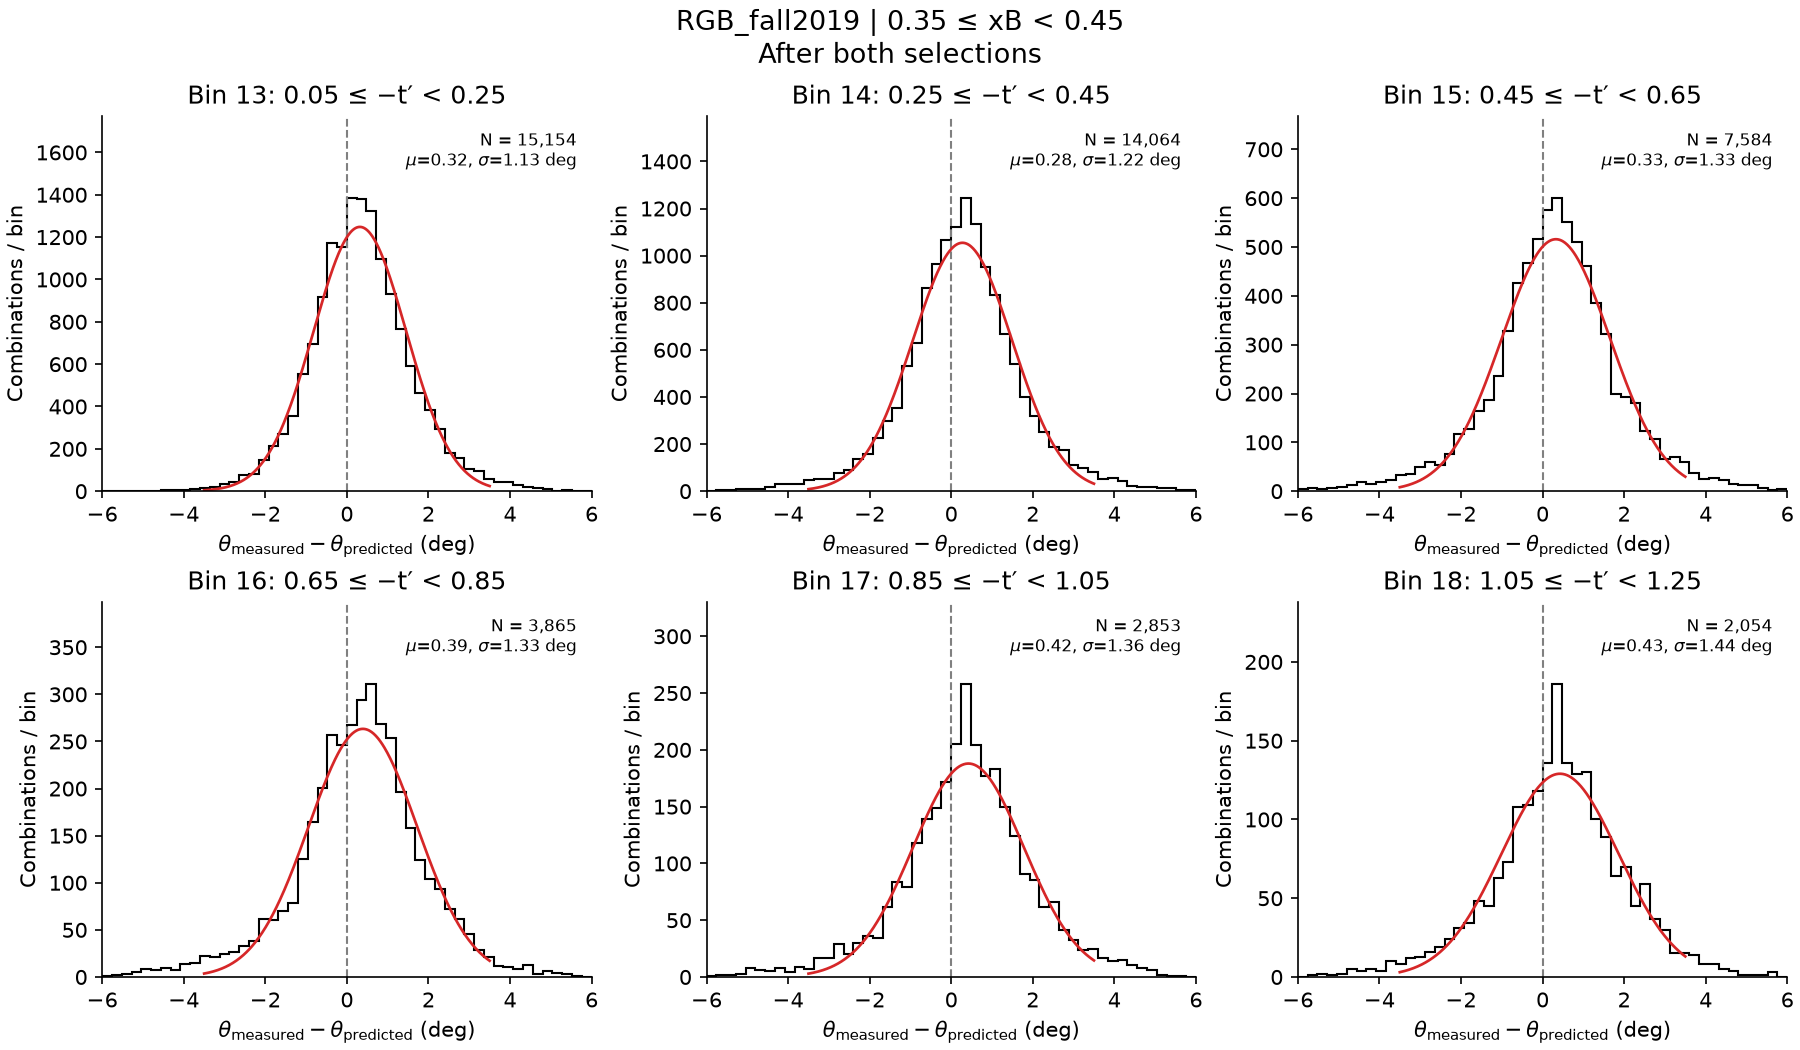
\includegraphics[width=\linewidth]{figures/channel_selection/exclusivity/rgb_fa19_angle_xb3.png}
\caption{RGB\_fall2019: pion polar-angle closure after both cuts in $x_B$ interval 3. The panels retain the six fine selection bins.}\label{fig:new_excl_rgb_fa19_angle3}
\end{figure}
\clearpage
\begin{figure}[p]\centering
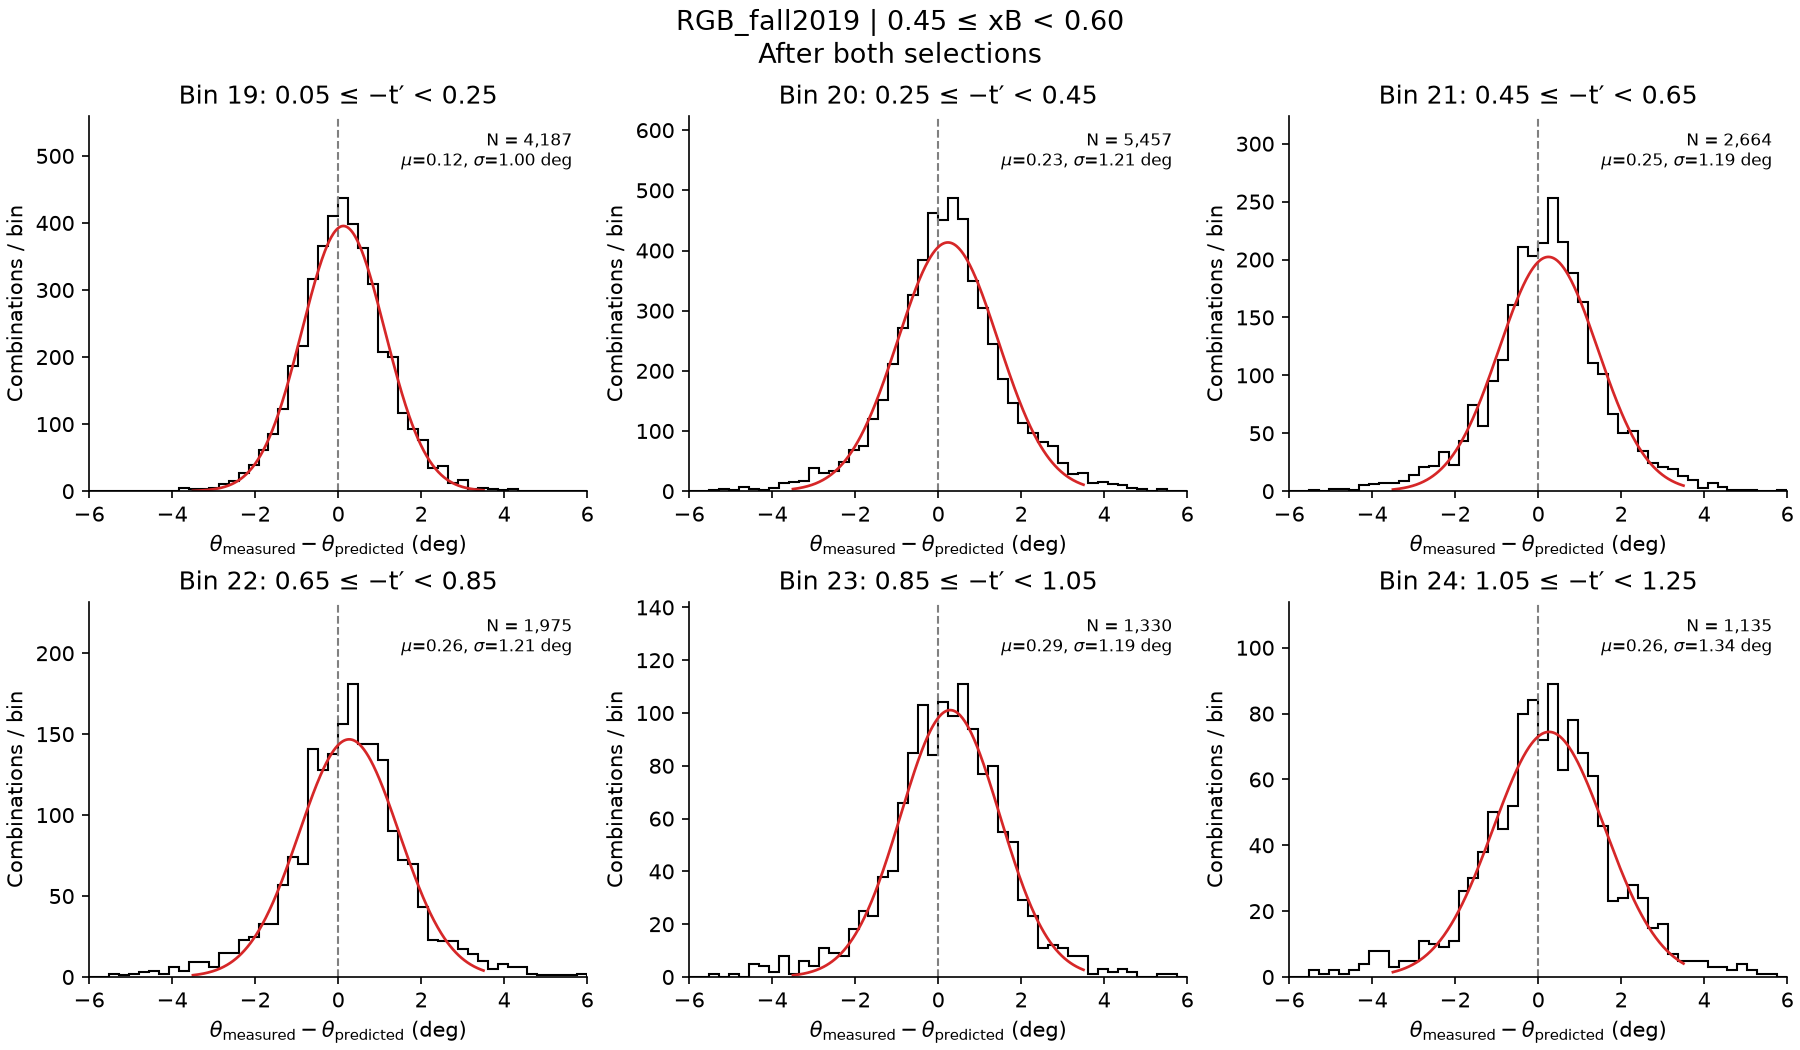
\includegraphics[width=\linewidth]{figures/channel_selection/exclusivity/rgb_fa19_angle_xb4.png}
\caption{RGB\_fall2019: pion polar-angle closure after both cuts in $x_B$ interval 4. The panels retain the six fine selection bins.}\label{fig:new_excl_rgb_fa19_angle4}
\end{figure}
\clearpage
\begin{figure}[p]\centering
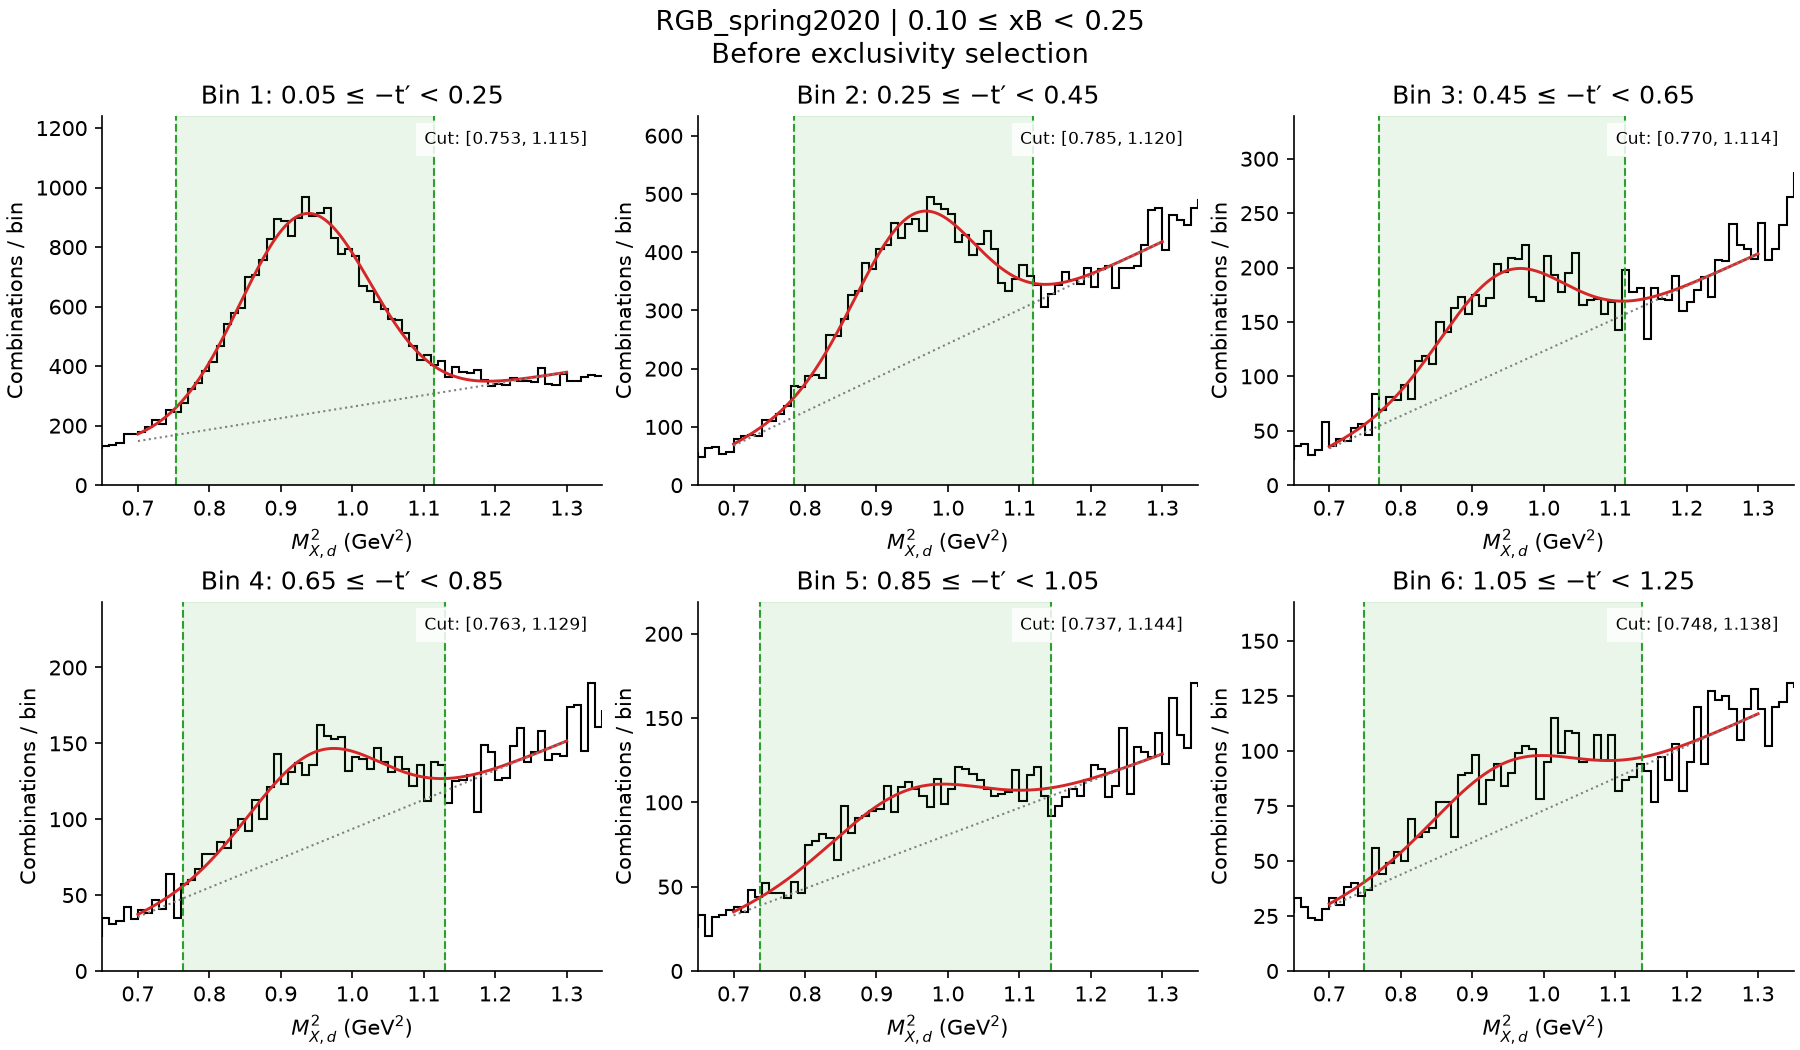
\includegraphics[width=\linewidth]{figures/channel_selection/exclusivity/rgb_sp20_mass_xb1.png}
\caption{RGB\_spring2020: deuteron-reference missing-mass-squared fits in $x_B$ interval 1. The panels retain the six fine selection bins.}\label{fig:new_excl_rgb_sp20_mass1}
\end{figure}
\clearpage
\begin{figure}[p]\centering
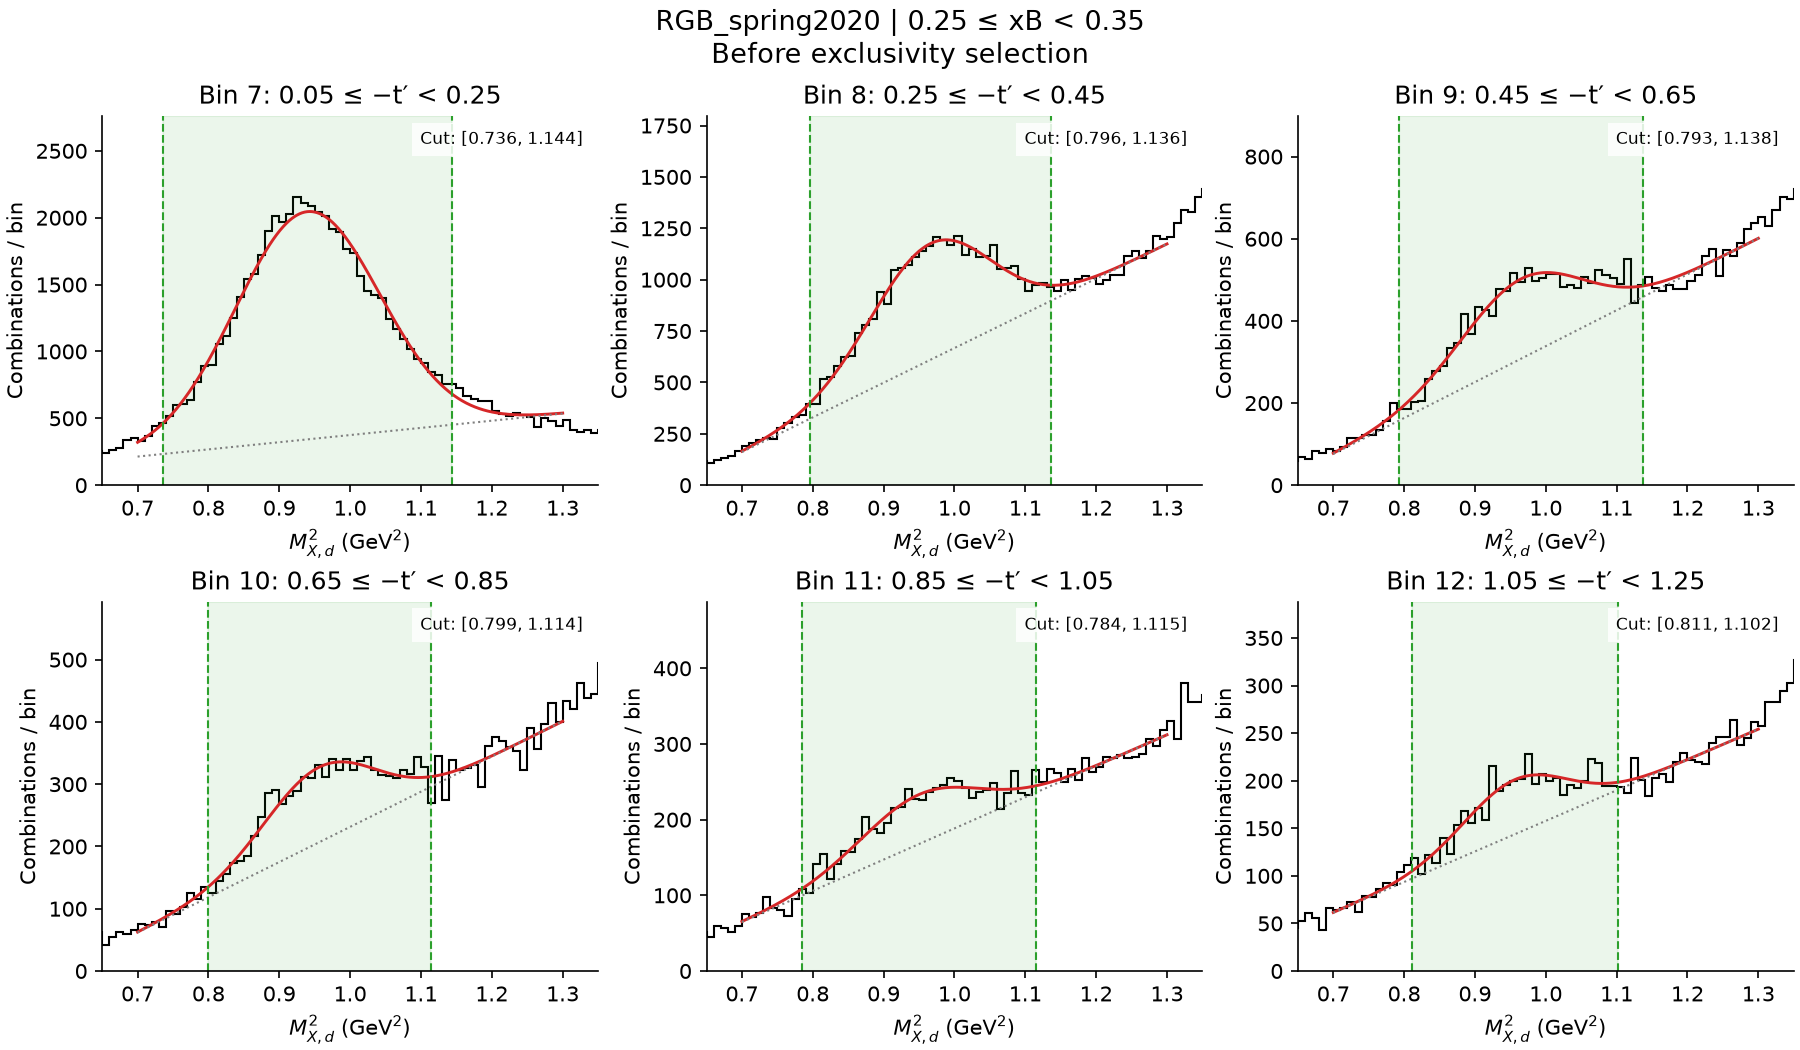
\includegraphics[width=\linewidth]{figures/channel_selection/exclusivity/rgb_sp20_mass_xb2.png}
\caption{RGB\_spring2020: deuteron-reference missing-mass-squared fits in $x_B$ interval 2. The panels retain the six fine selection bins.}\label{fig:new_excl_rgb_sp20_mass2}
\end{figure}
\clearpage
\begin{figure}[p]\centering
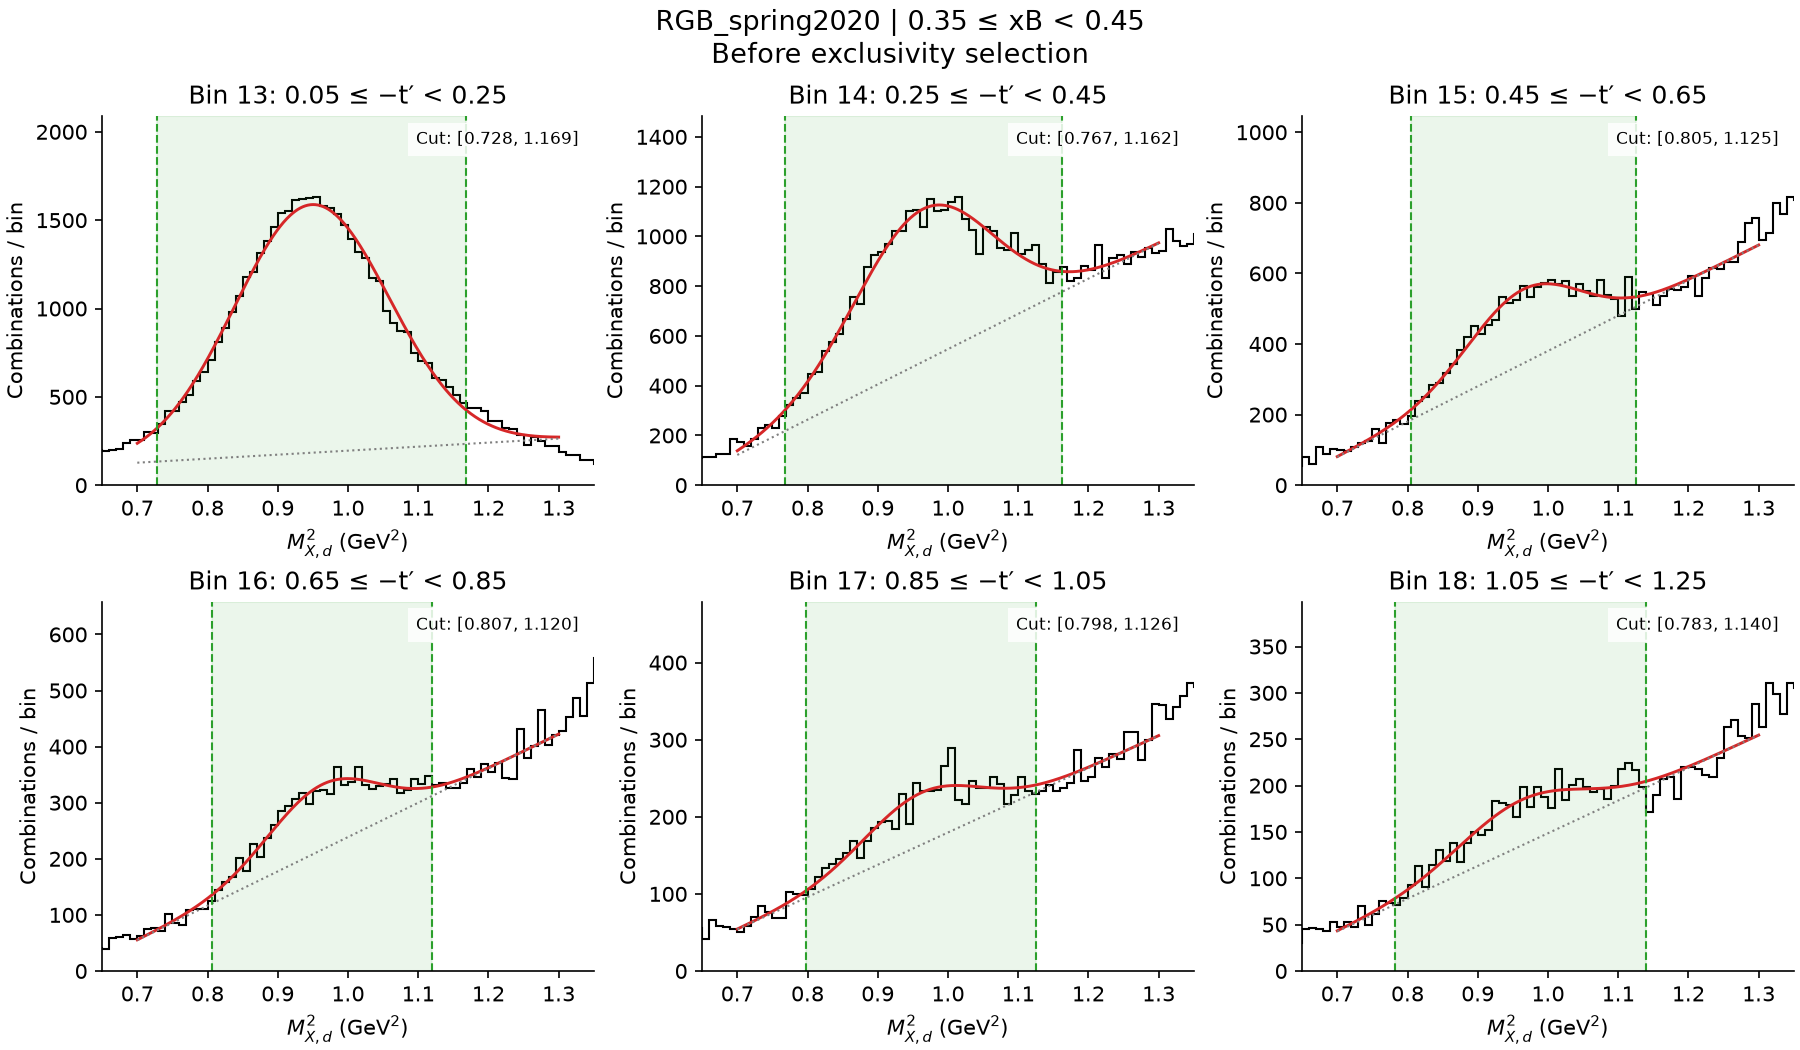
\includegraphics[width=\linewidth]{figures/channel_selection/exclusivity/rgb_sp20_mass_xb3.png}
\caption{RGB\_spring2020: deuteron-reference missing-mass-squared fits in $x_B$ interval 3. The panels retain the six fine selection bins.}\label{fig:new_excl_rgb_sp20_mass3}
\end{figure}
\clearpage
\begin{figure}[p]\centering
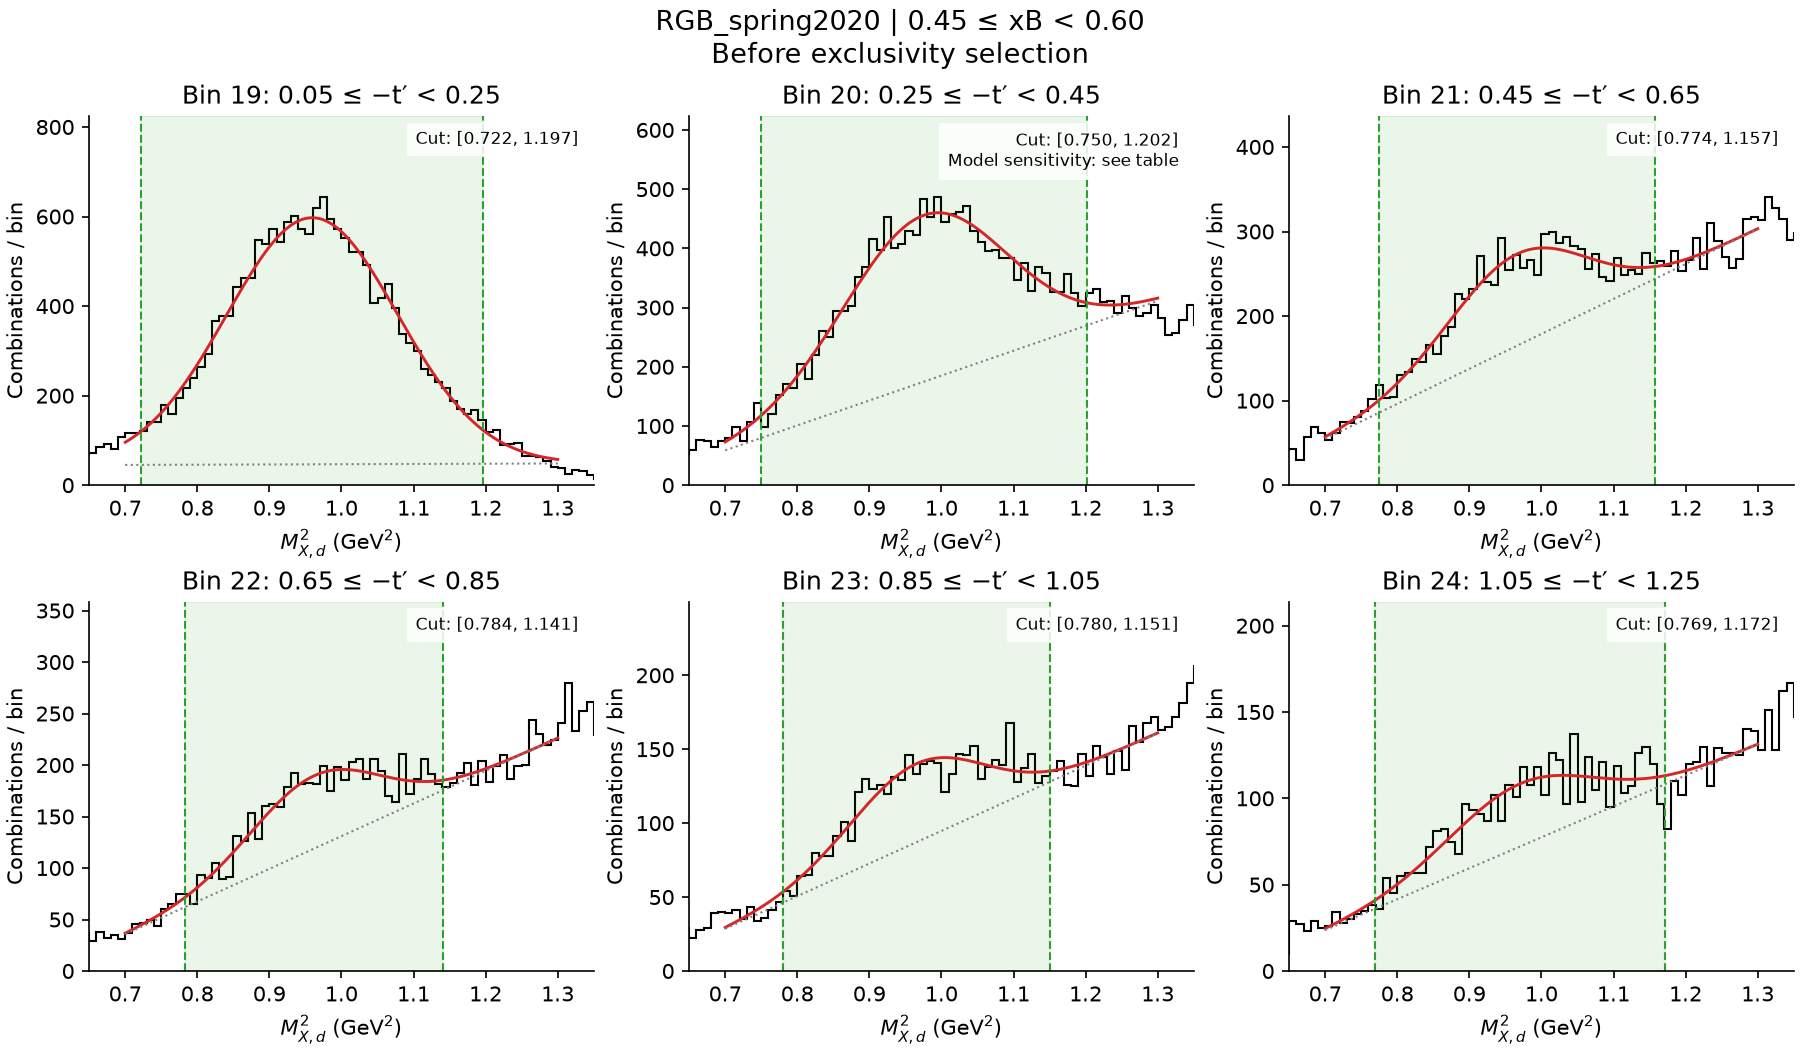
\includegraphics[width=\linewidth]{figures/channel_selection/exclusivity/rgb_sp20_mass_xb4.png}
\caption{RGB\_spring2020: deuteron-reference missing-mass-squared fits in $x_B$ interval 4. The panels retain the six fine selection bins.}\label{fig:new_excl_rgb_sp20_mass4}
\end{figure}
\clearpage
\begin{figure}[p]\centering
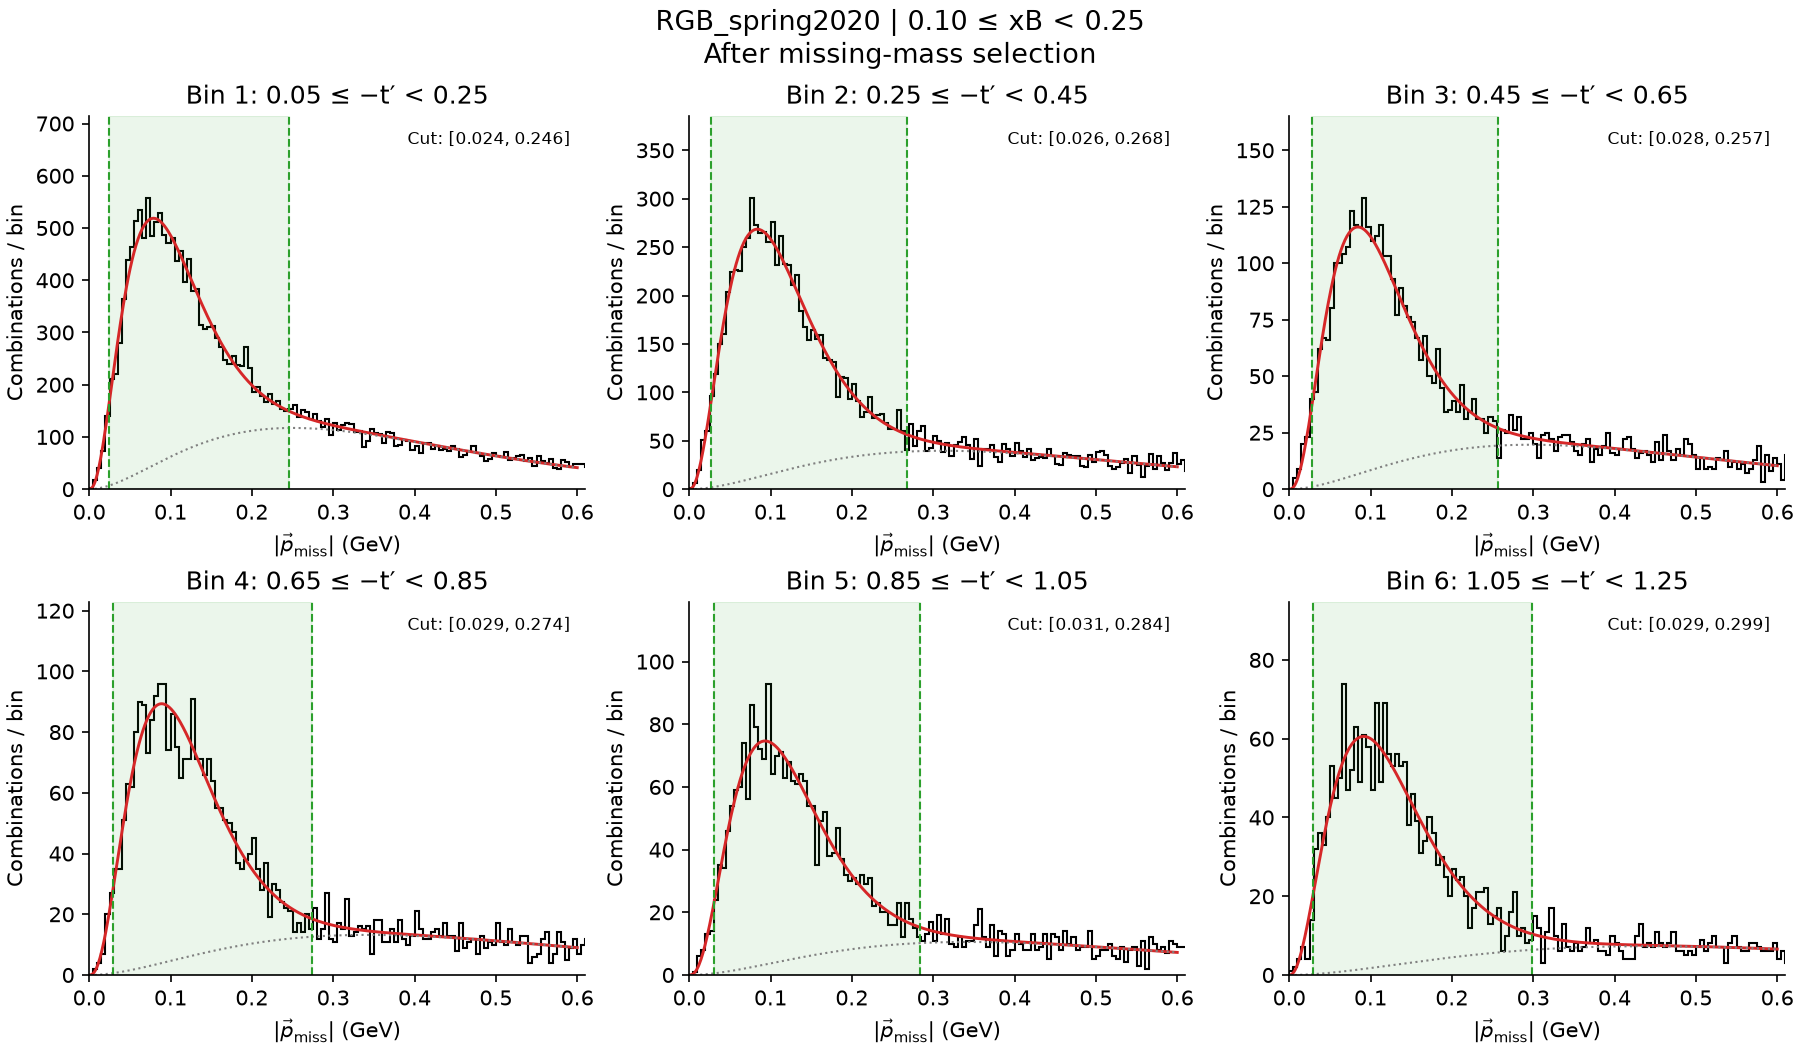
\includegraphics[width=\linewidth]{figures/channel_selection/exclusivity/rgb_sp20_momentum_xb1.png}
\caption{RGB\_spring2020: missing-momentum fits after the mass cut in $x_B$ interval 1. The panels retain the six fine selection bins.}\label{fig:new_excl_rgb_sp20_momentum1}
\end{figure}
\clearpage
\begin{figure}[p]\centering
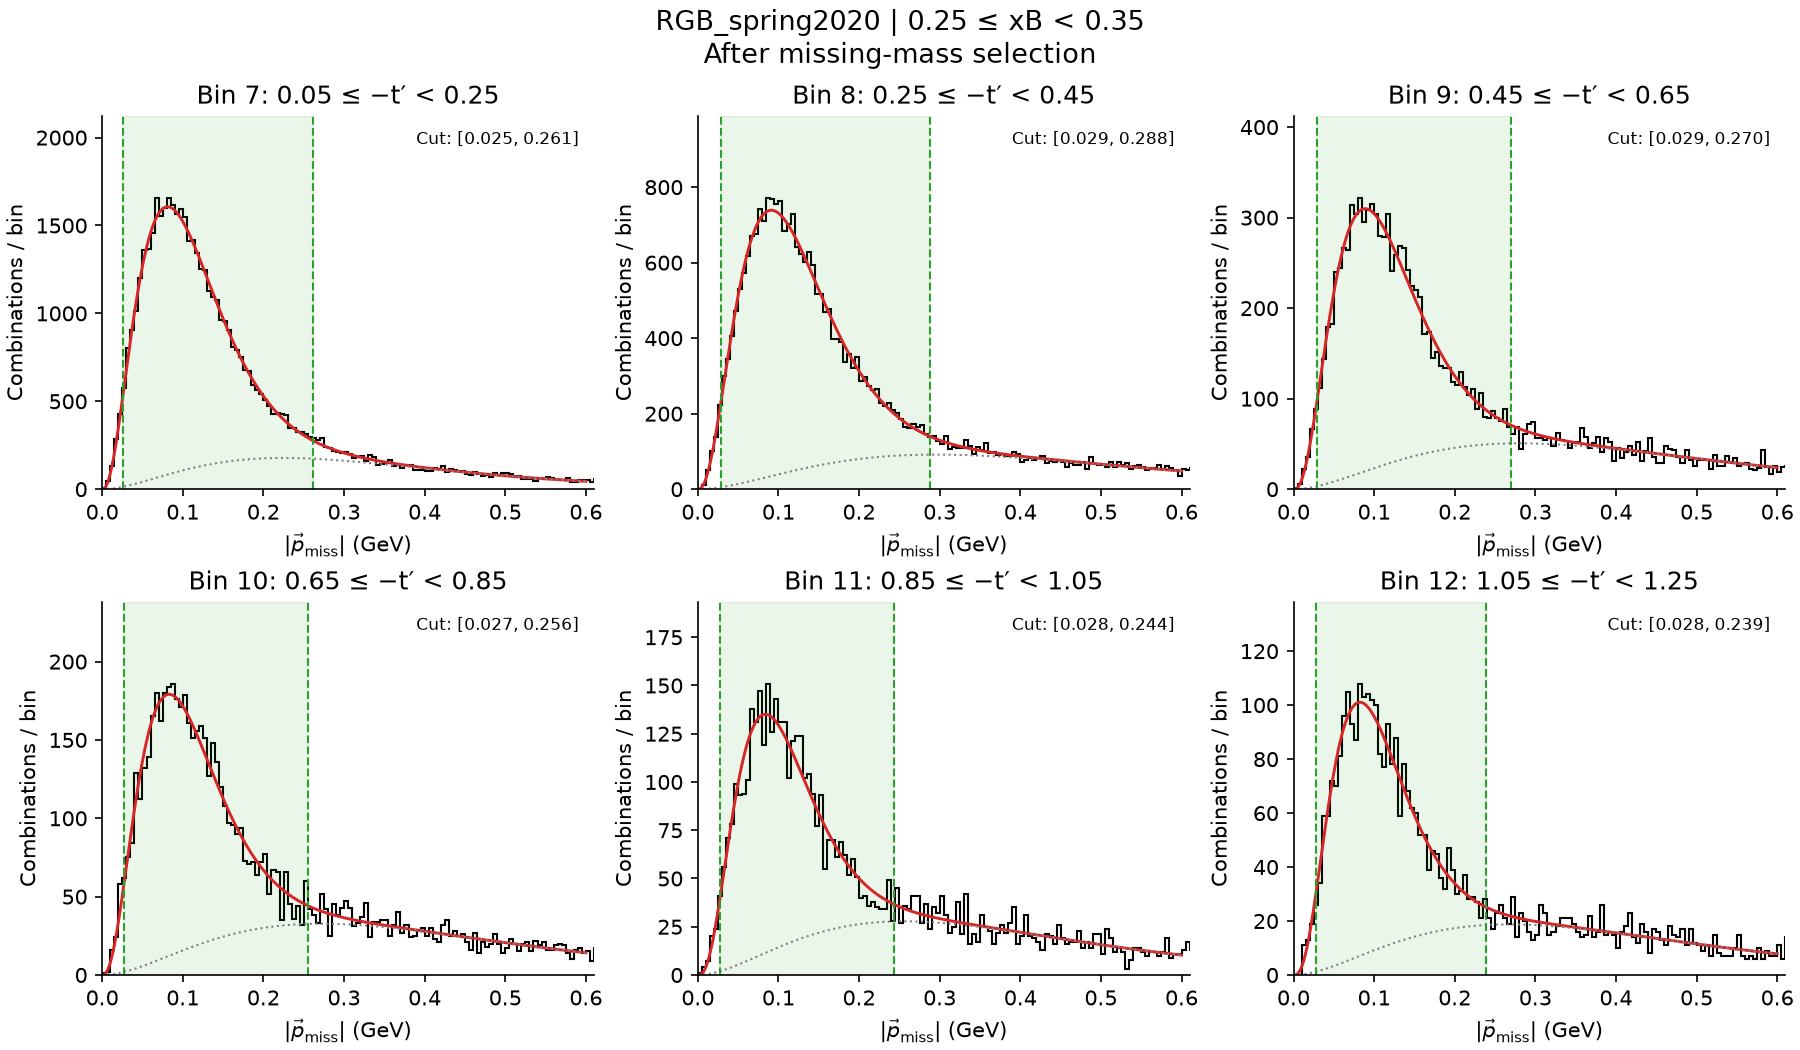
\includegraphics[width=\linewidth]{figures/channel_selection/exclusivity/rgb_sp20_momentum_xb2.png}
\caption{RGB\_spring2020: missing-momentum fits after the mass cut in $x_B$ interval 2. The panels retain the six fine selection bins.}\label{fig:new_excl_rgb_sp20_momentum2}
\end{figure}
\clearpage
\begin{figure}[p]\centering
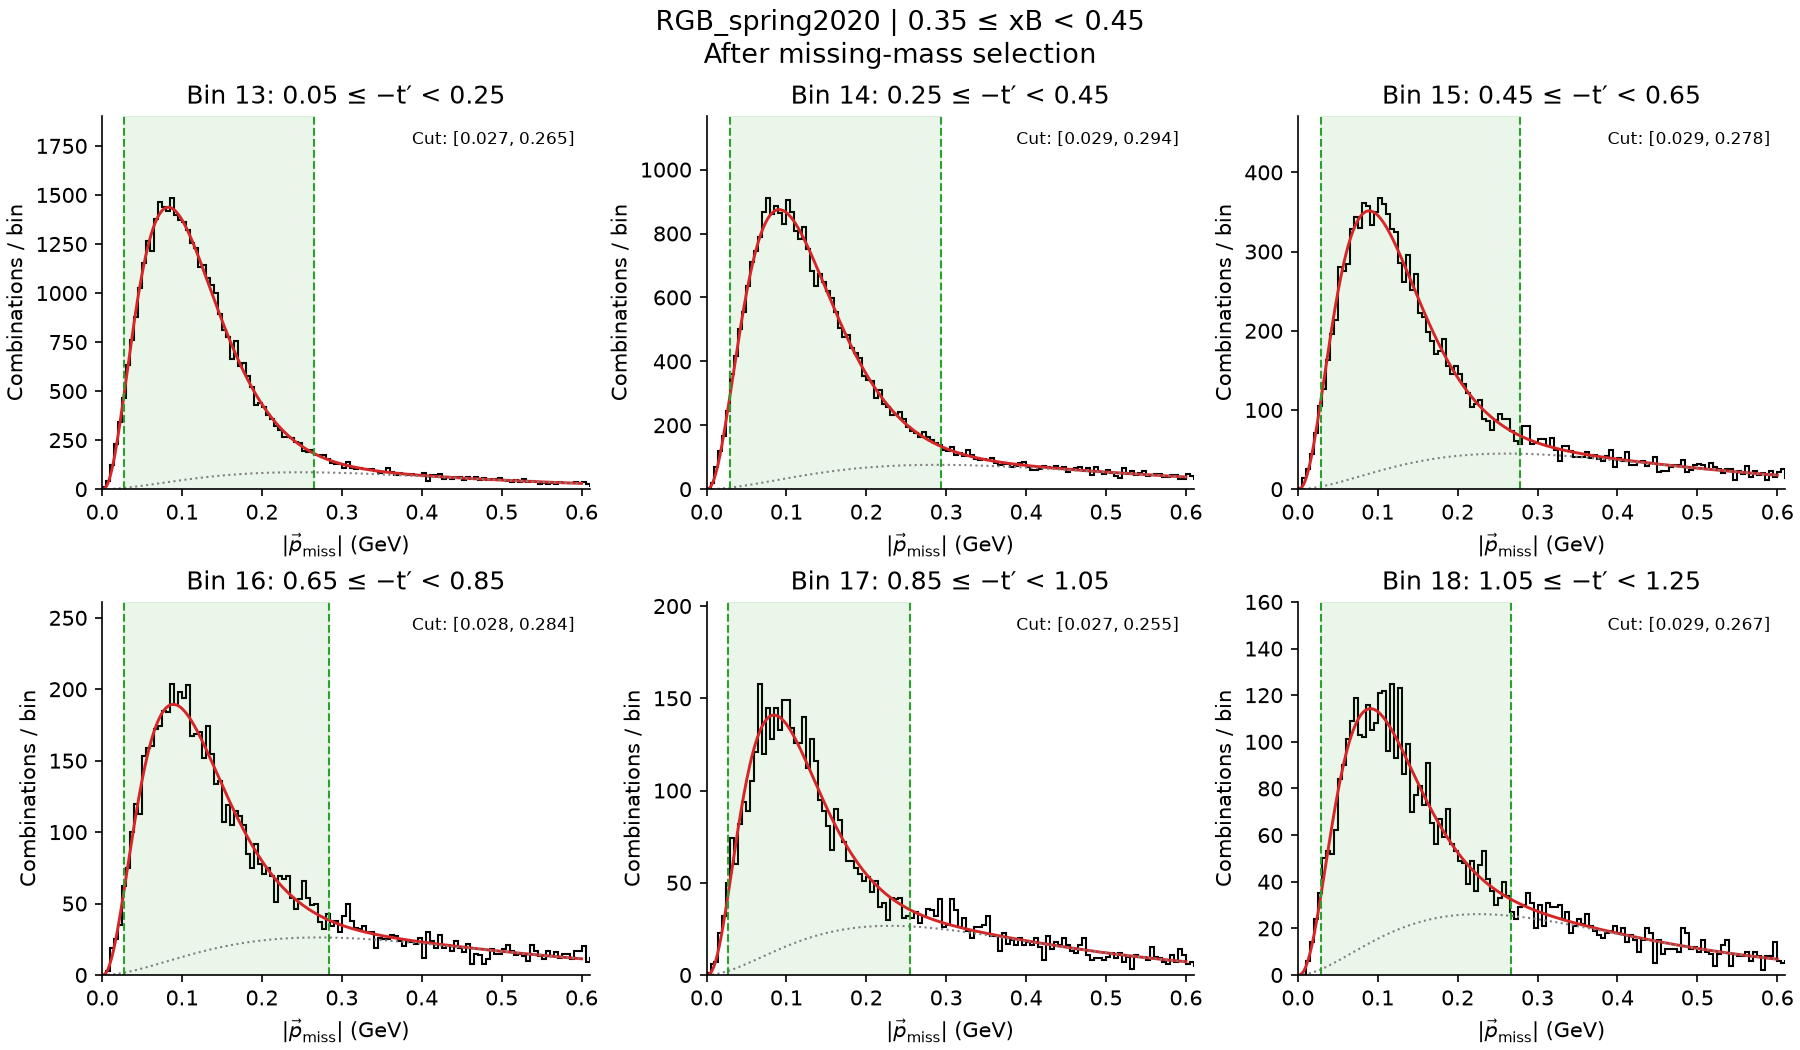
\includegraphics[width=\linewidth]{figures/channel_selection/exclusivity/rgb_sp20_momentum_xb3.png}
\caption{RGB\_spring2020: missing-momentum fits after the mass cut in $x_B$ interval 3. The panels retain the six fine selection bins.}\label{fig:new_excl_rgb_sp20_momentum3}
\end{figure}
\clearpage
\begin{figure}[p]\centering
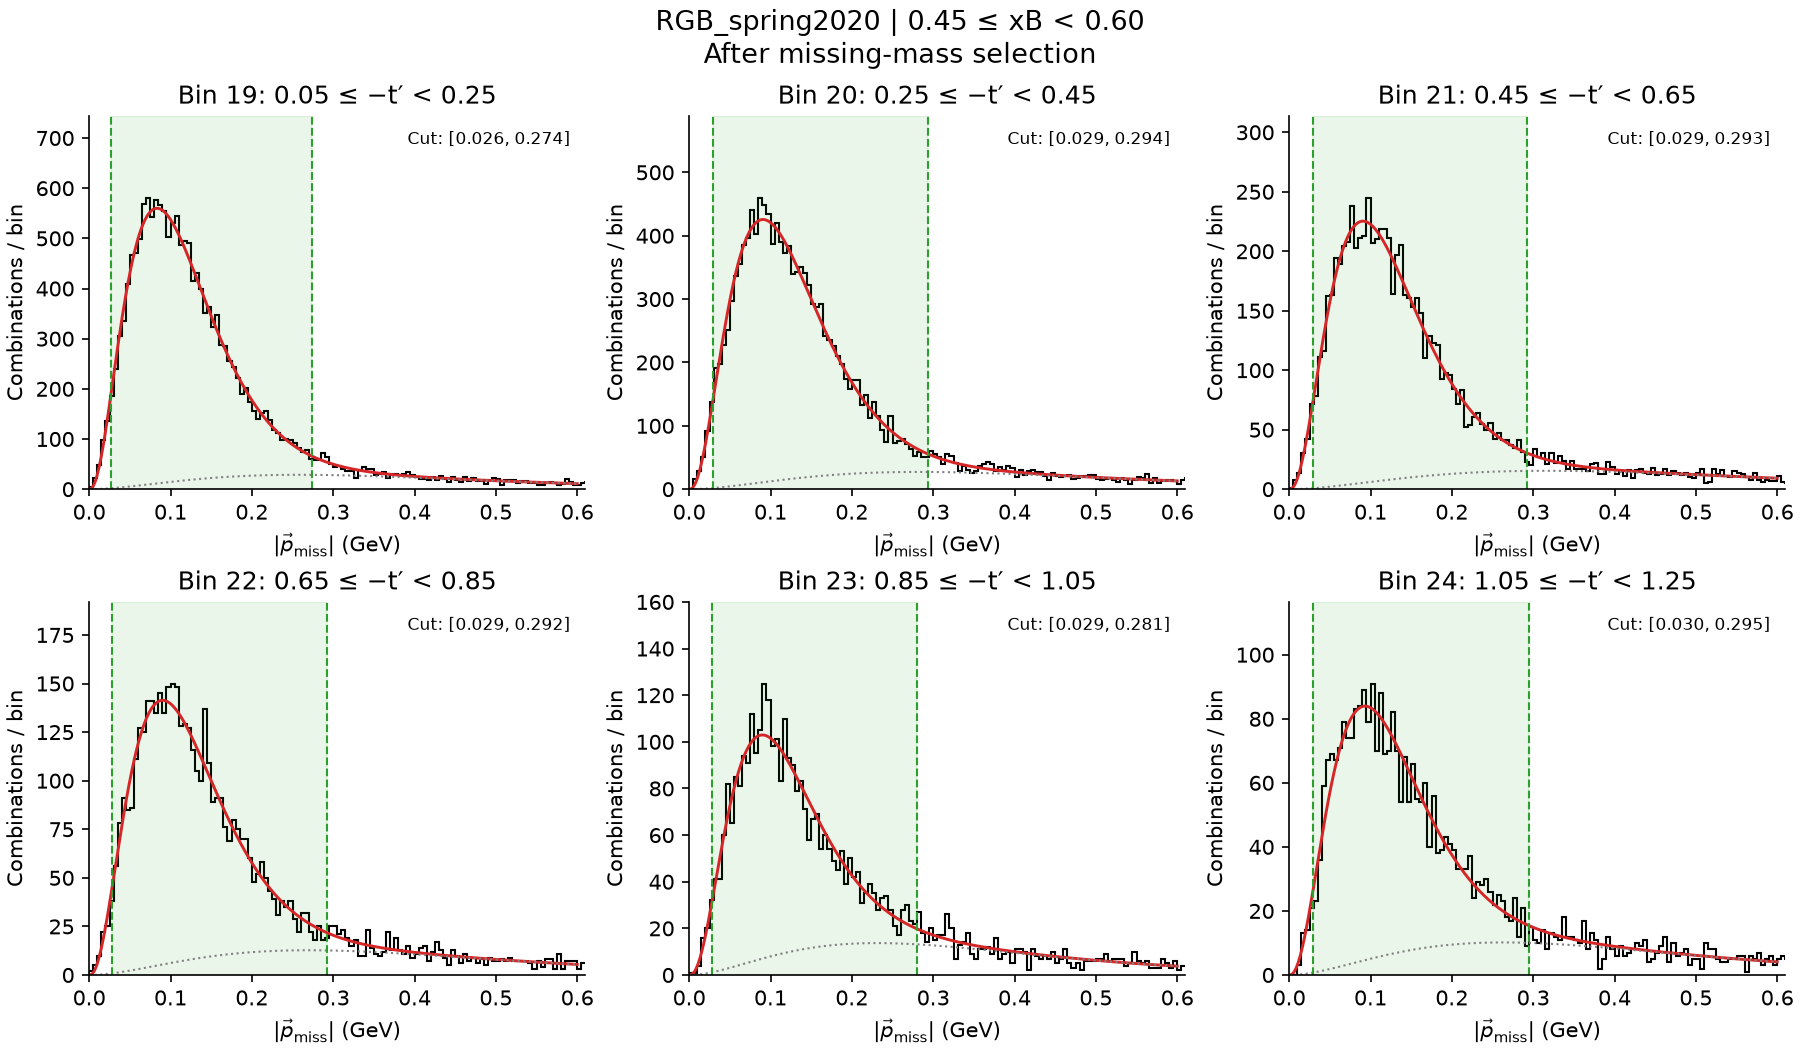
\includegraphics[width=\linewidth]{figures/channel_selection/exclusivity/rgb_sp20_momentum_xb4.png}
\caption{RGB\_spring2020: missing-momentum fits after the mass cut in $x_B$ interval 4. The panels retain the six fine selection bins.}\label{fig:new_excl_rgb_sp20_momentum4}
\end{figure}
\clearpage
\begin{figure}[p]\centering
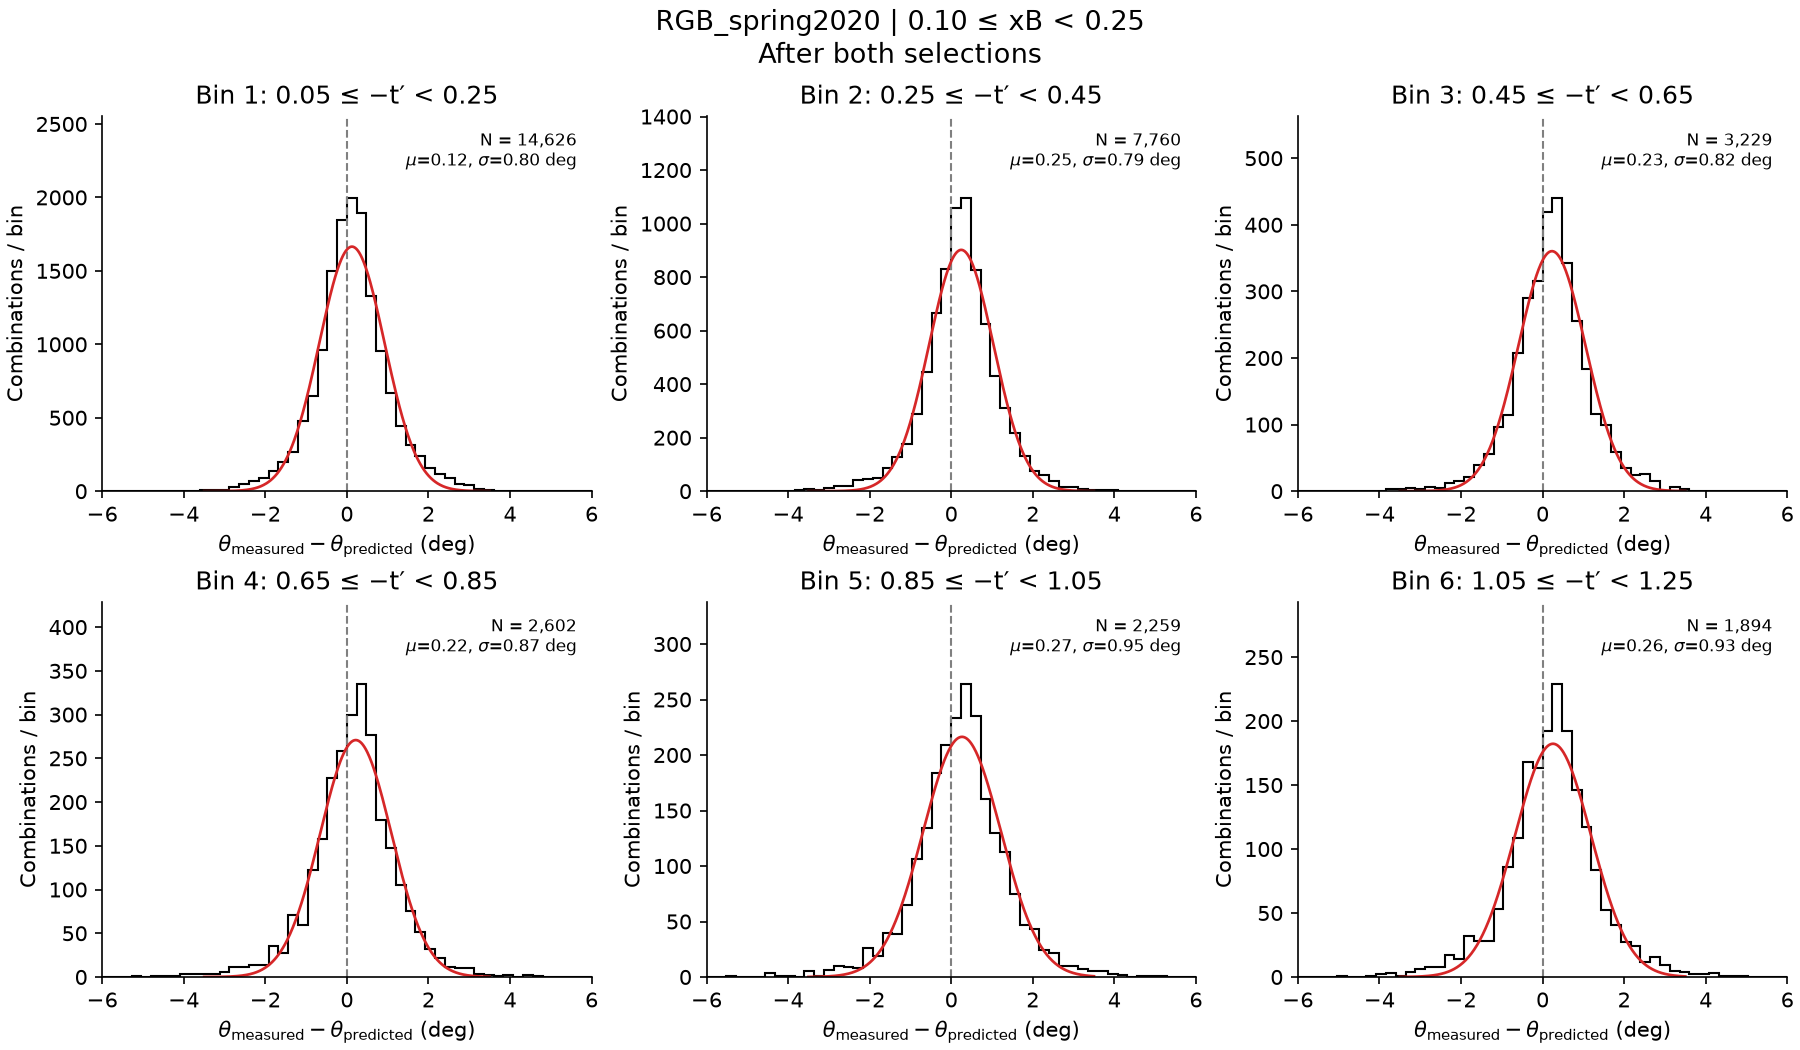
\includegraphics[width=\linewidth]{figures/channel_selection/exclusivity/rgb_sp20_angle_xb1.png}
\caption{RGB\_spring2020: pion polar-angle closure after both cuts in $x_B$ interval 1. The panels retain the six fine selection bins.}\label{fig:new_excl_rgb_sp20_angle1}
\end{figure}
\clearpage
\begin{figure}[p]\centering
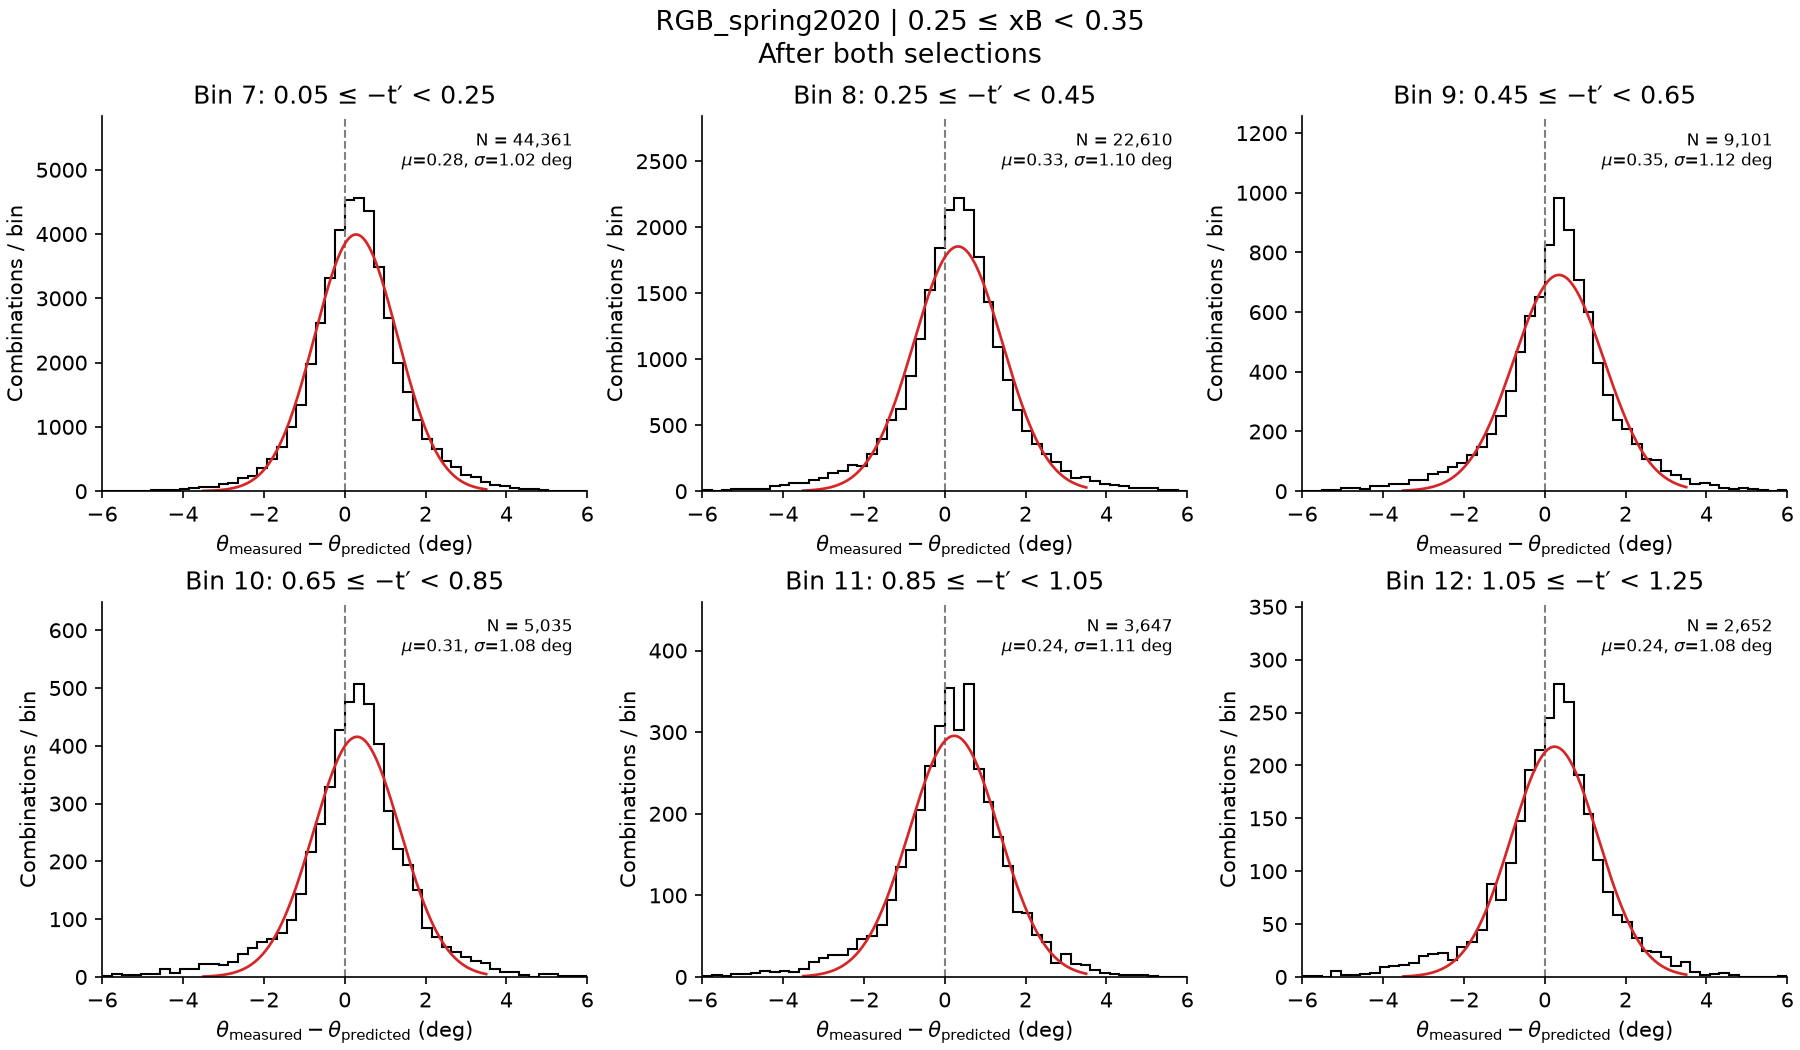
\includegraphics[width=\linewidth]{figures/channel_selection/exclusivity/rgb_sp20_angle_xb2.png}
\caption{RGB\_spring2020: pion polar-angle closure after both cuts in $x_B$ interval 2. The panels retain the six fine selection bins.}\label{fig:new_excl_rgb_sp20_angle2}
\end{figure}
\clearpage
\begin{figure}[p]\centering
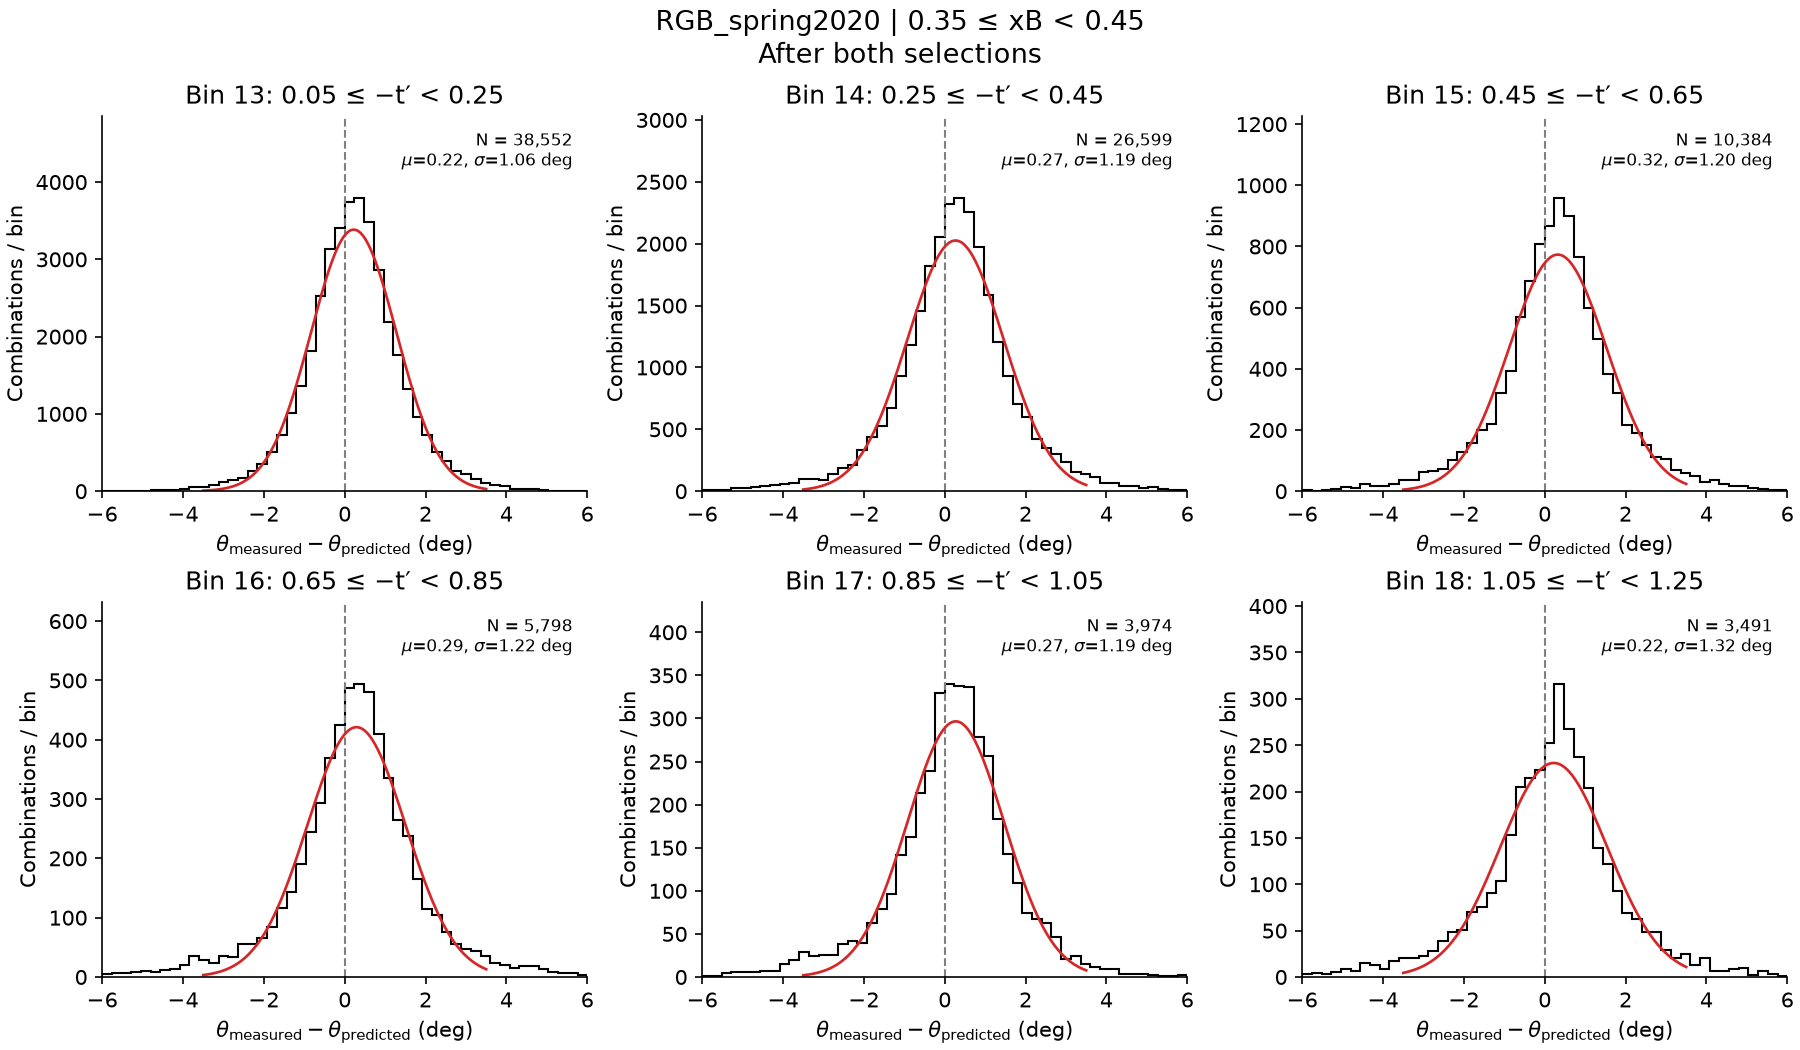
\includegraphics[width=\linewidth]{figures/channel_selection/exclusivity/rgb_sp20_angle_xb3.png}
\caption{RGB\_spring2020: pion polar-angle closure after both cuts in $x_B$ interval 3. The panels retain the six fine selection bins.}\label{fig:new_excl_rgb_sp20_angle3}
\end{figure}
\clearpage
\begin{figure}[p]\centering
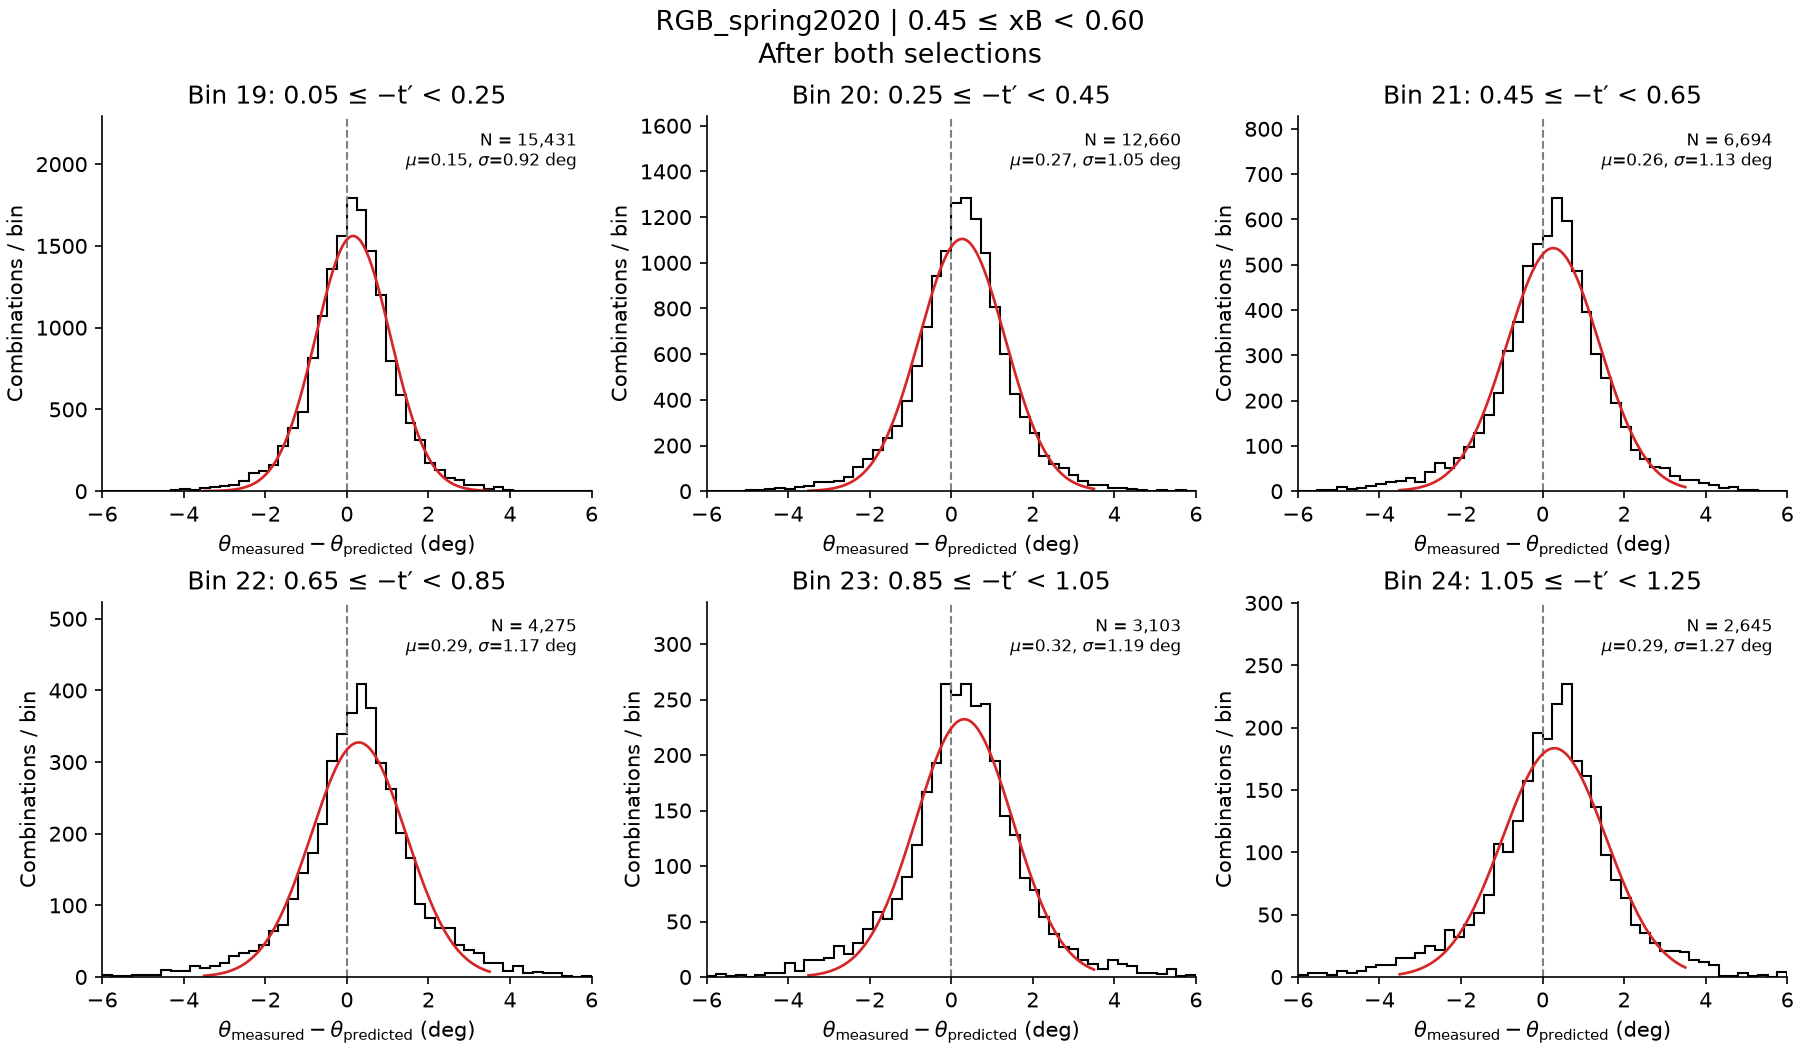
\includegraphics[width=\linewidth]{figures/channel_selection/exclusivity/rgb_sp20_angle_xb4.png}
\caption{RGB\_spring2020: pion polar-angle closure after both cuts in $x_B$ interval 4. The panels retain the six fine selection bins.}\label{fig:new_excl_rgb_sp20_angle4}
\end{figure}
\clearpage
\begin{figure}[p]\centering
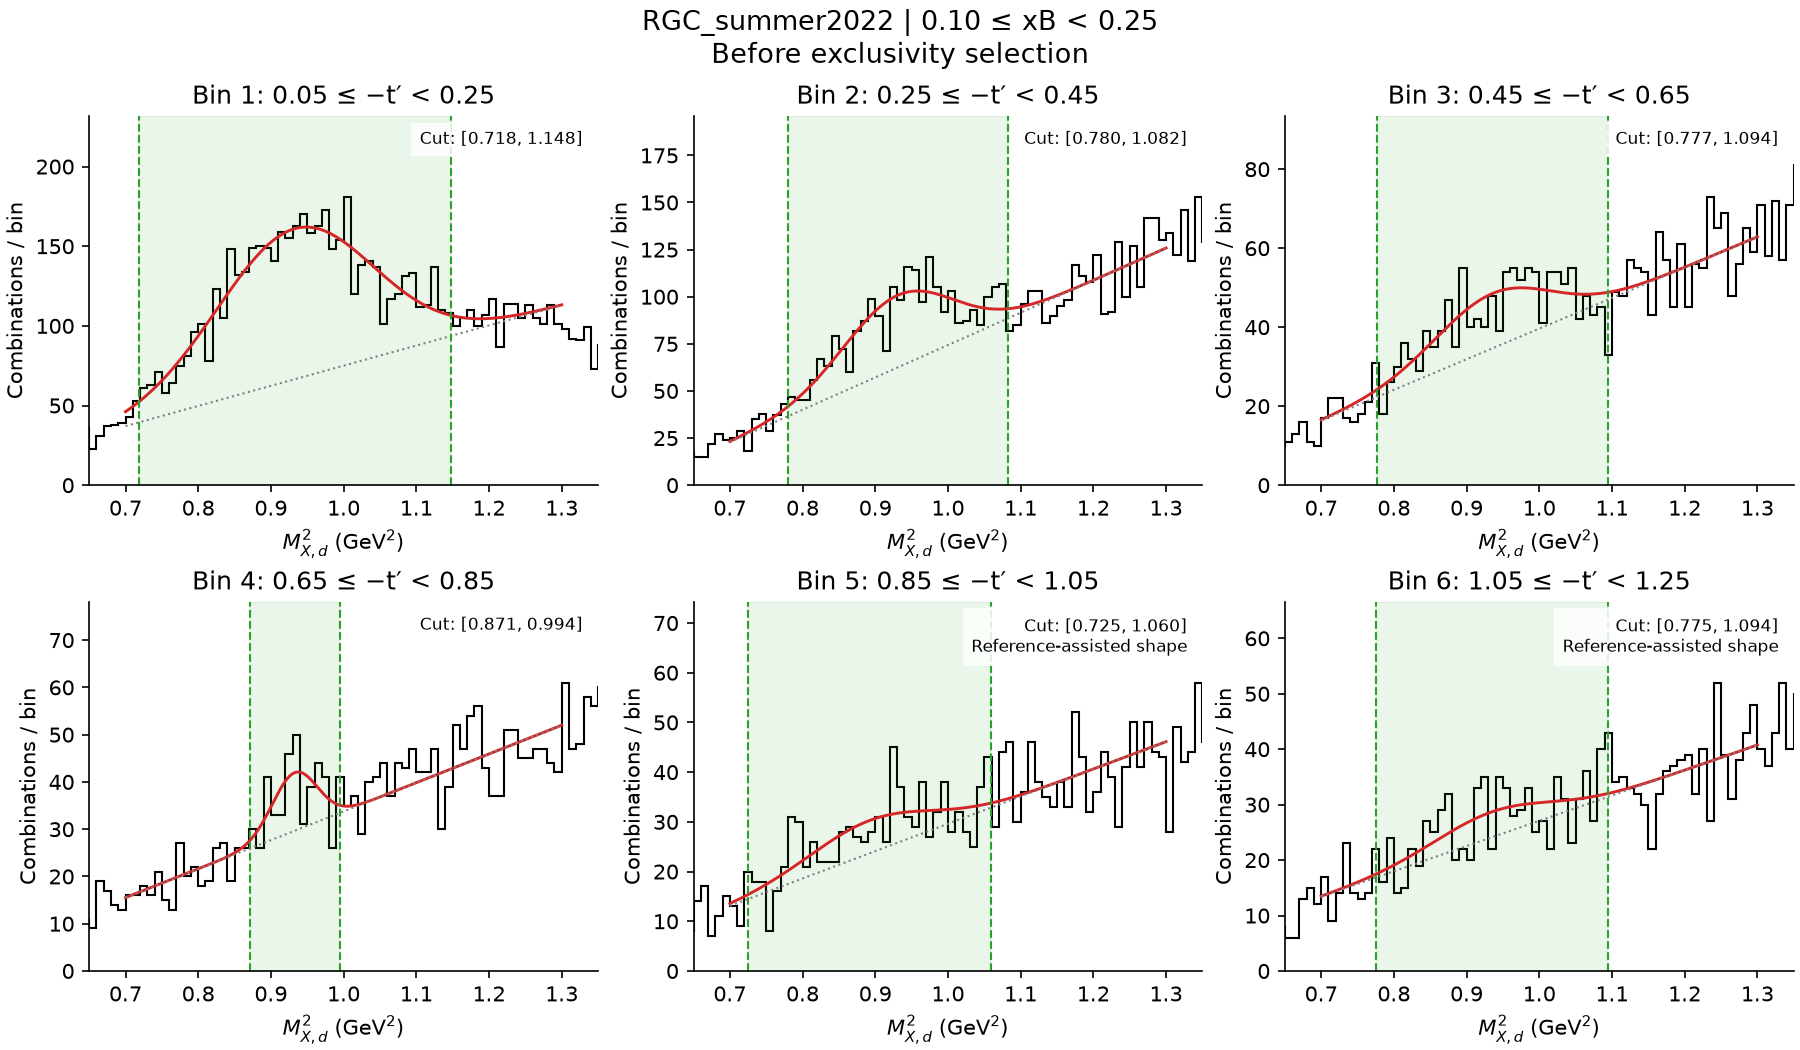
\includegraphics[width=\linewidth]{figures/channel_selection/exclusivity/rgc_su22_mass_xb1.png}
\caption{RGC\_summer2022: deuteron-reference missing-mass-squared fits in $x_B$ interval 1. The panels retain the six fine selection bins.}\label{fig:new_excl_rgc_su22_mass1}
\end{figure}
\clearpage
\begin{figure}[p]\centering
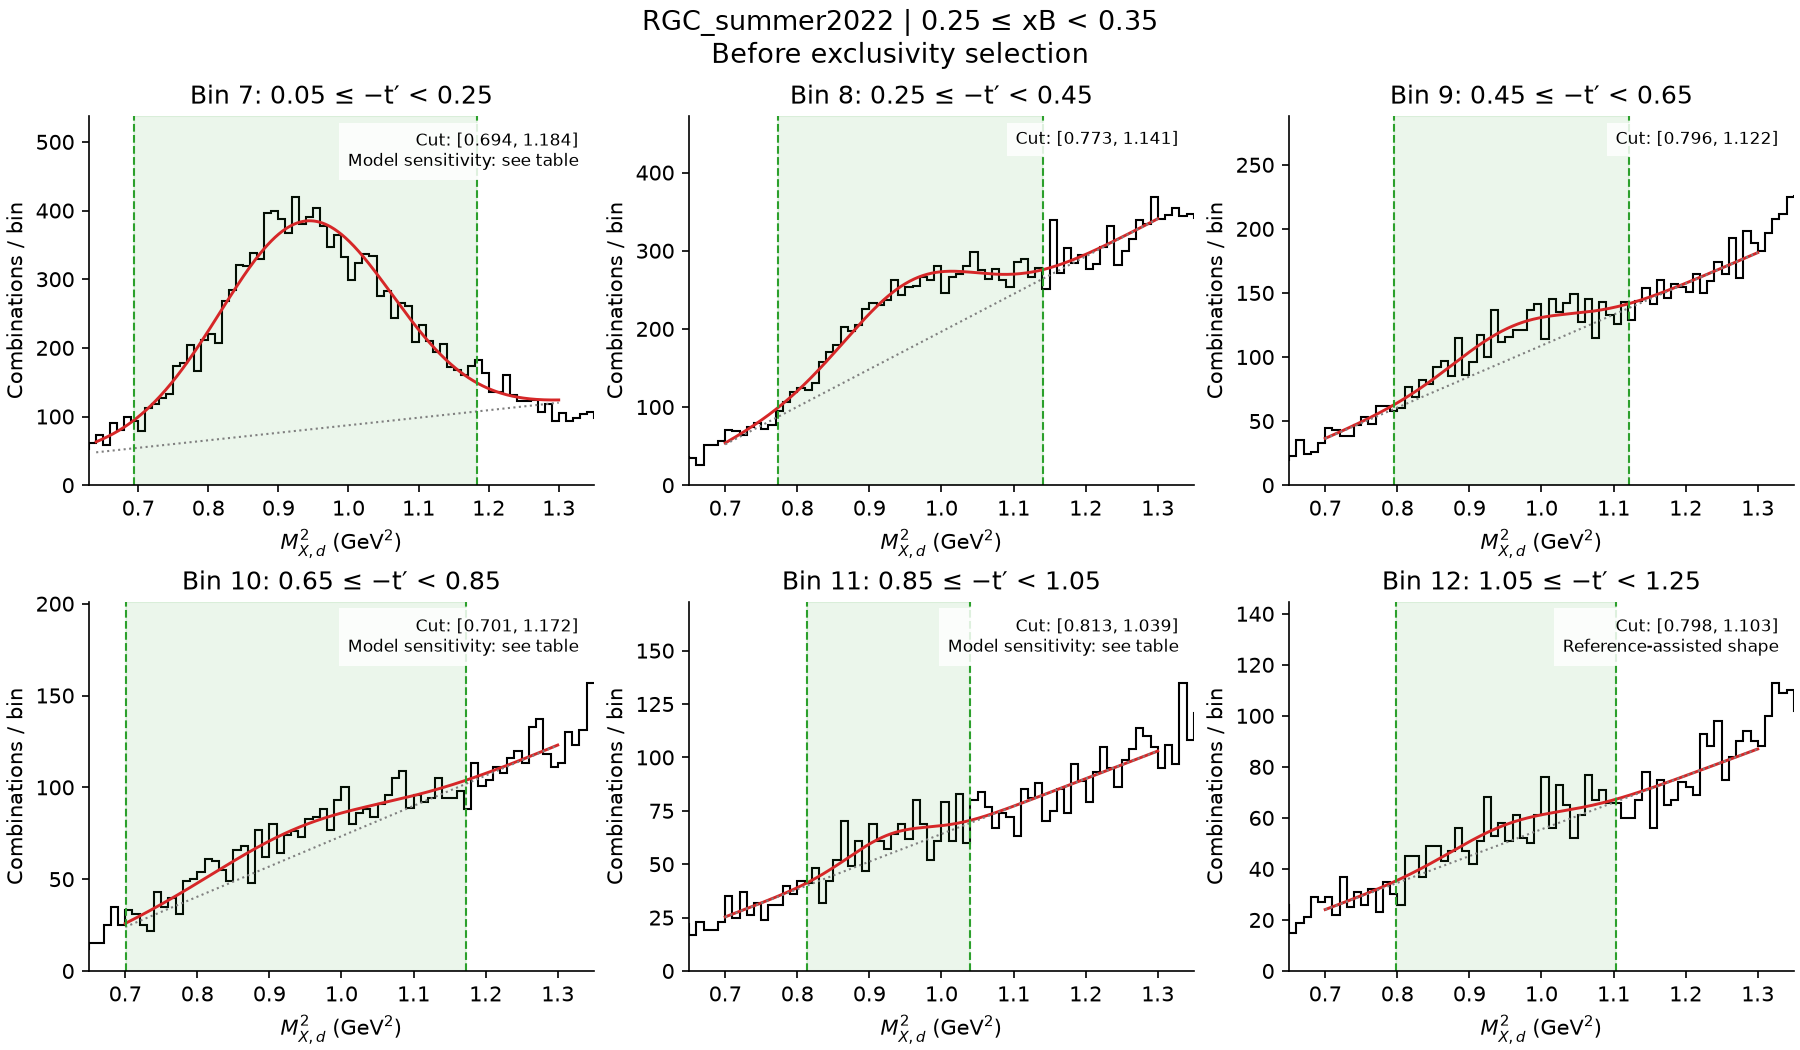
\includegraphics[width=\linewidth]{figures/channel_selection/exclusivity/rgc_su22_mass_xb2.png}
\caption{RGC\_summer2022: deuteron-reference missing-mass-squared fits in $x_B$ interval 2. The panels retain the six fine selection bins.}\label{fig:new_excl_rgc_su22_mass2}
\end{figure}
\clearpage
\begin{figure}[p]\centering
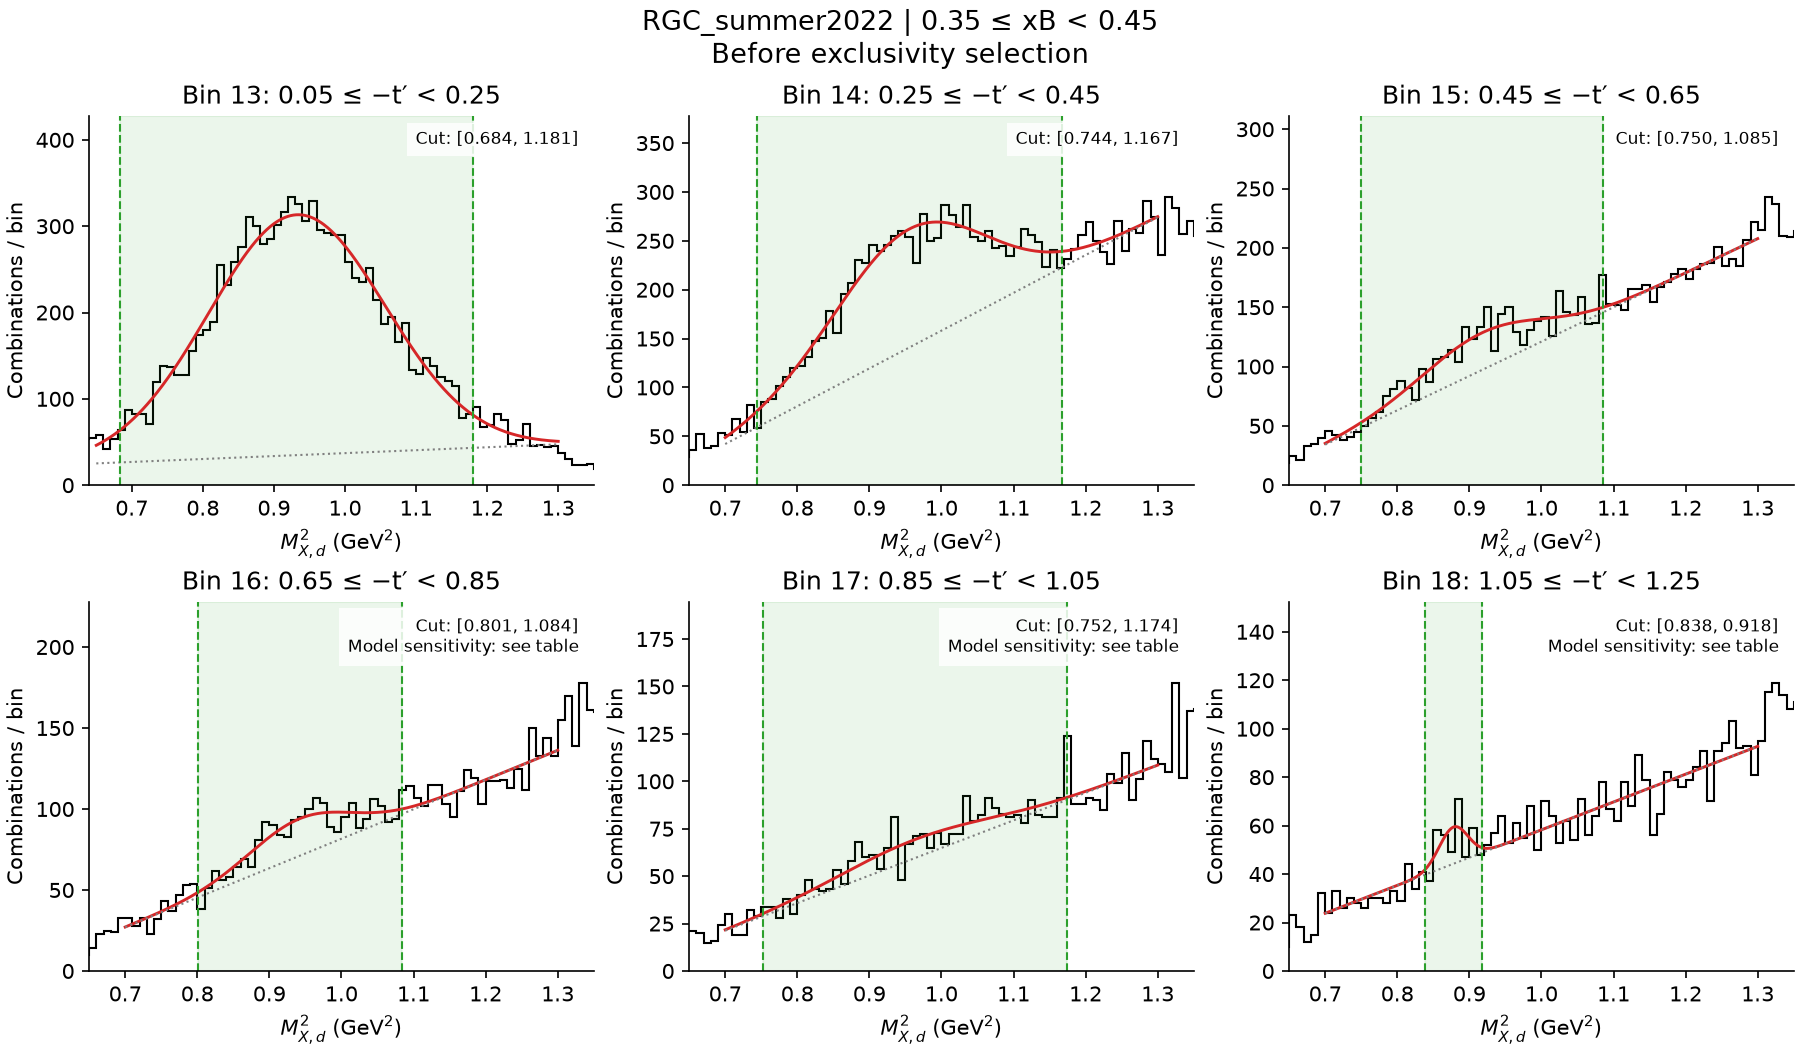
\includegraphics[width=\linewidth]{figures/channel_selection/exclusivity/rgc_su22_mass_xb3.png}
\caption{RGC\_summer2022: deuteron-reference missing-mass-squared fits in $x_B$ interval 3. The panels retain the six fine selection bins.}\label{fig:new_excl_rgc_su22_mass3}
\end{figure}
\clearpage
\begin{figure}[p]\centering
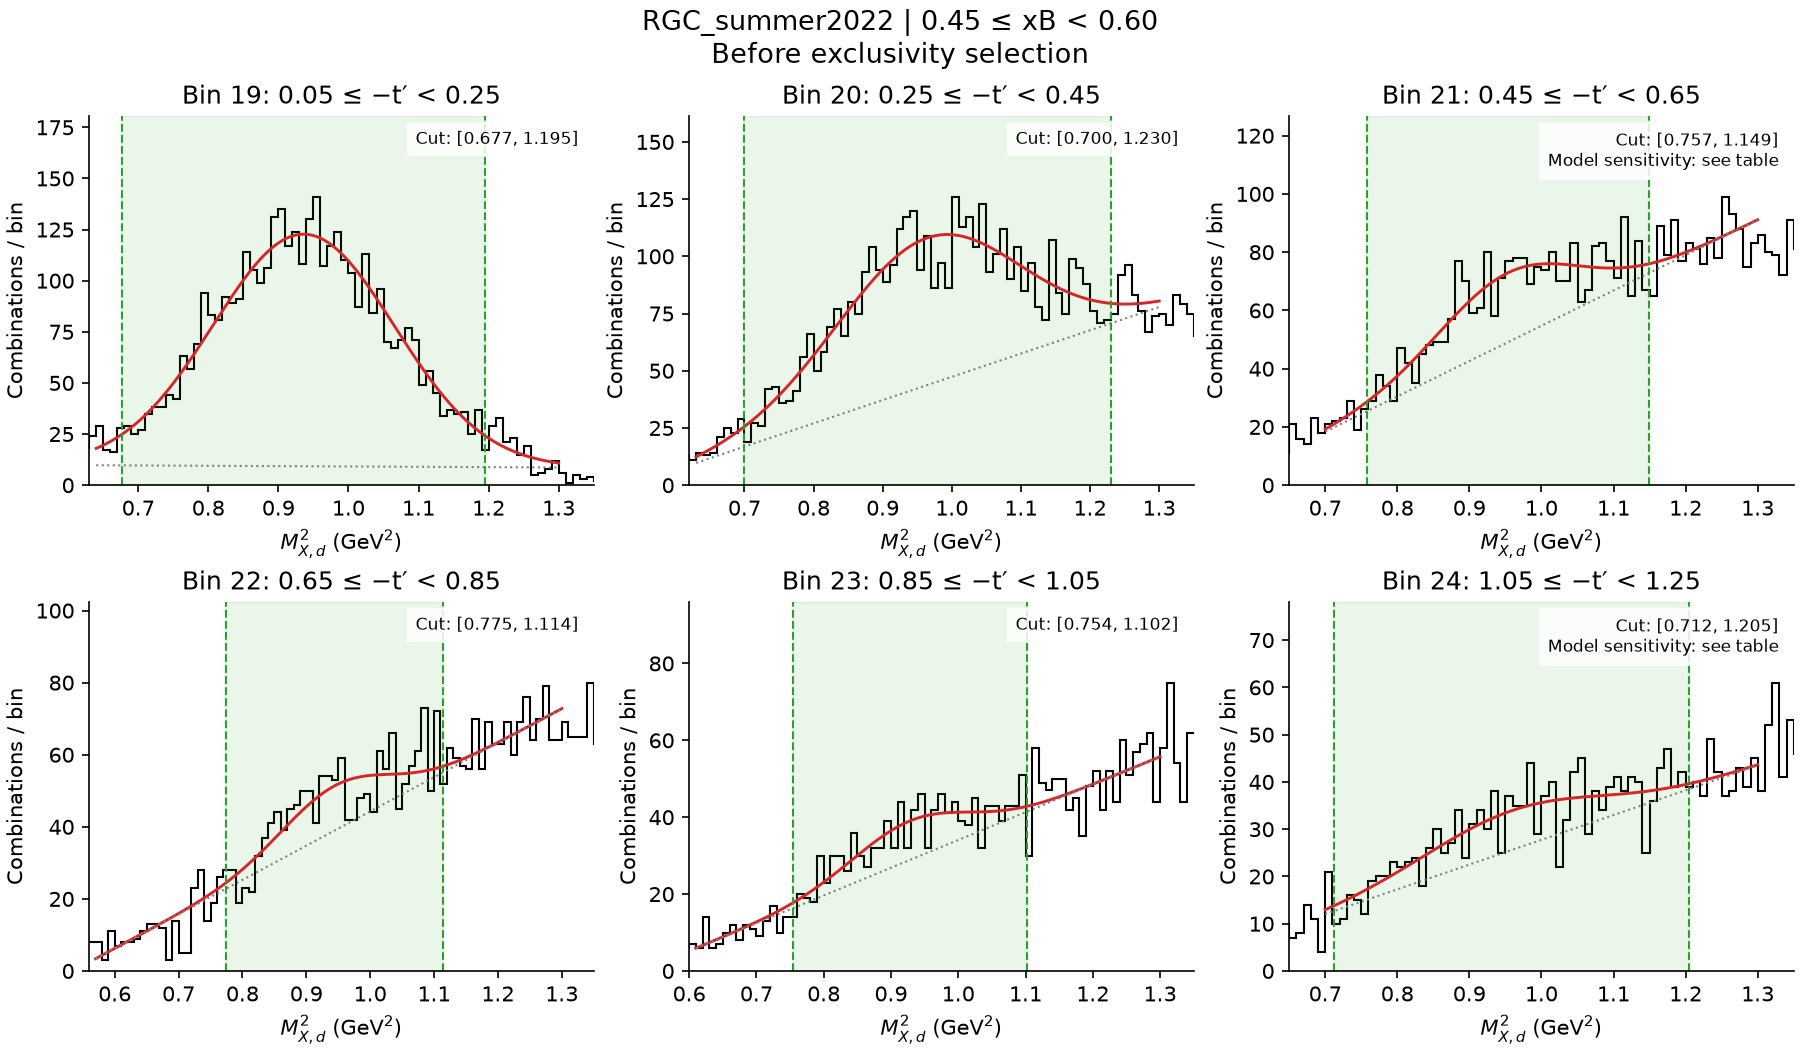
\includegraphics[width=\linewidth]{figures/channel_selection/exclusivity/rgc_su22_mass_xb4.png}
\caption{RGC\_summer2022: deuteron-reference missing-mass-squared fits in $x_B$ interval 4. The panels retain the six fine selection bins.}\label{fig:new_excl_rgc_su22_mass4}
\end{figure}
\clearpage
\begin{figure}[p]\centering
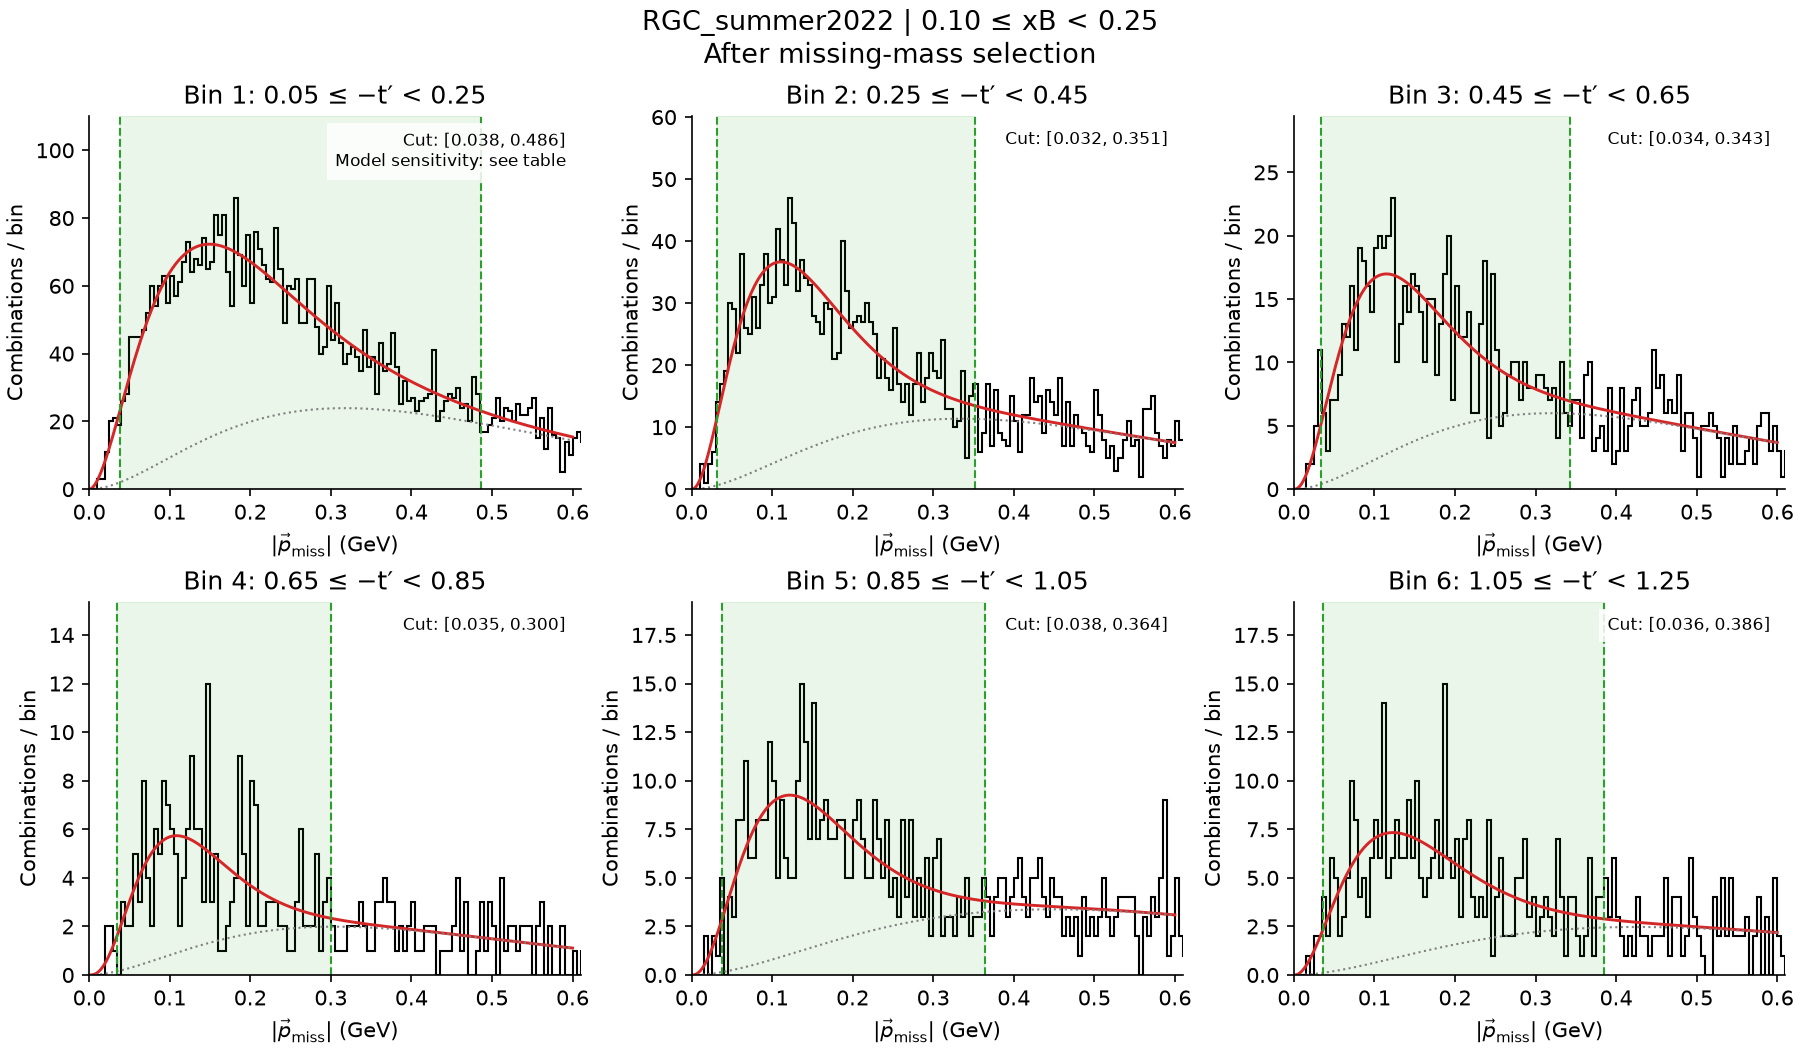
\includegraphics[width=\linewidth]{figures/channel_selection/exclusivity/rgc_su22_momentum_xb1.png}
\caption{RGC\_summer2022: missing-momentum fits after the mass cut in $x_B$ interval 1. The panels retain the six fine selection bins.}\label{fig:new_excl_rgc_su22_momentum1}
\end{figure}
\clearpage
\begin{figure}[p]\centering
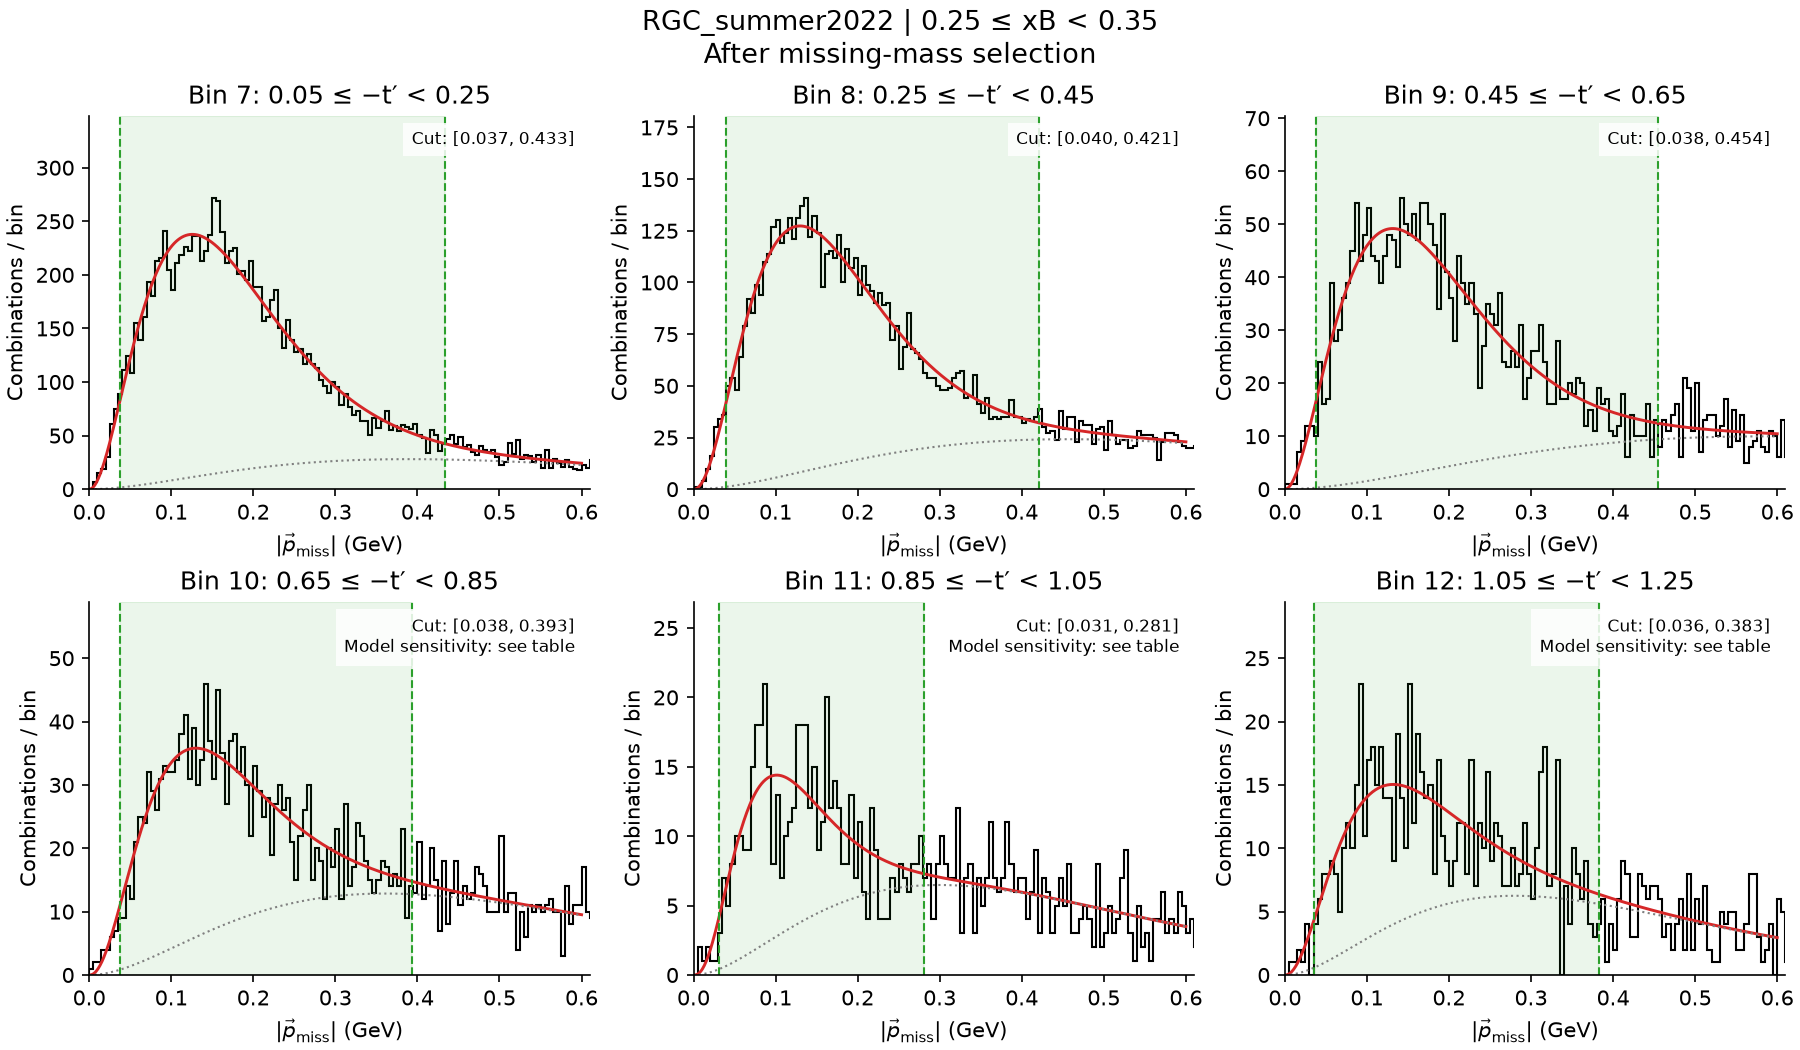
\includegraphics[width=\linewidth]{figures/channel_selection/exclusivity/rgc_su22_momentum_xb2.png}
\caption{RGC\_summer2022: missing-momentum fits after the mass cut in $x_B$ interval 2. The panels retain the six fine selection bins.}\label{fig:new_excl_rgc_su22_momentum2}
\end{figure}
\clearpage
\begin{figure}[p]\centering
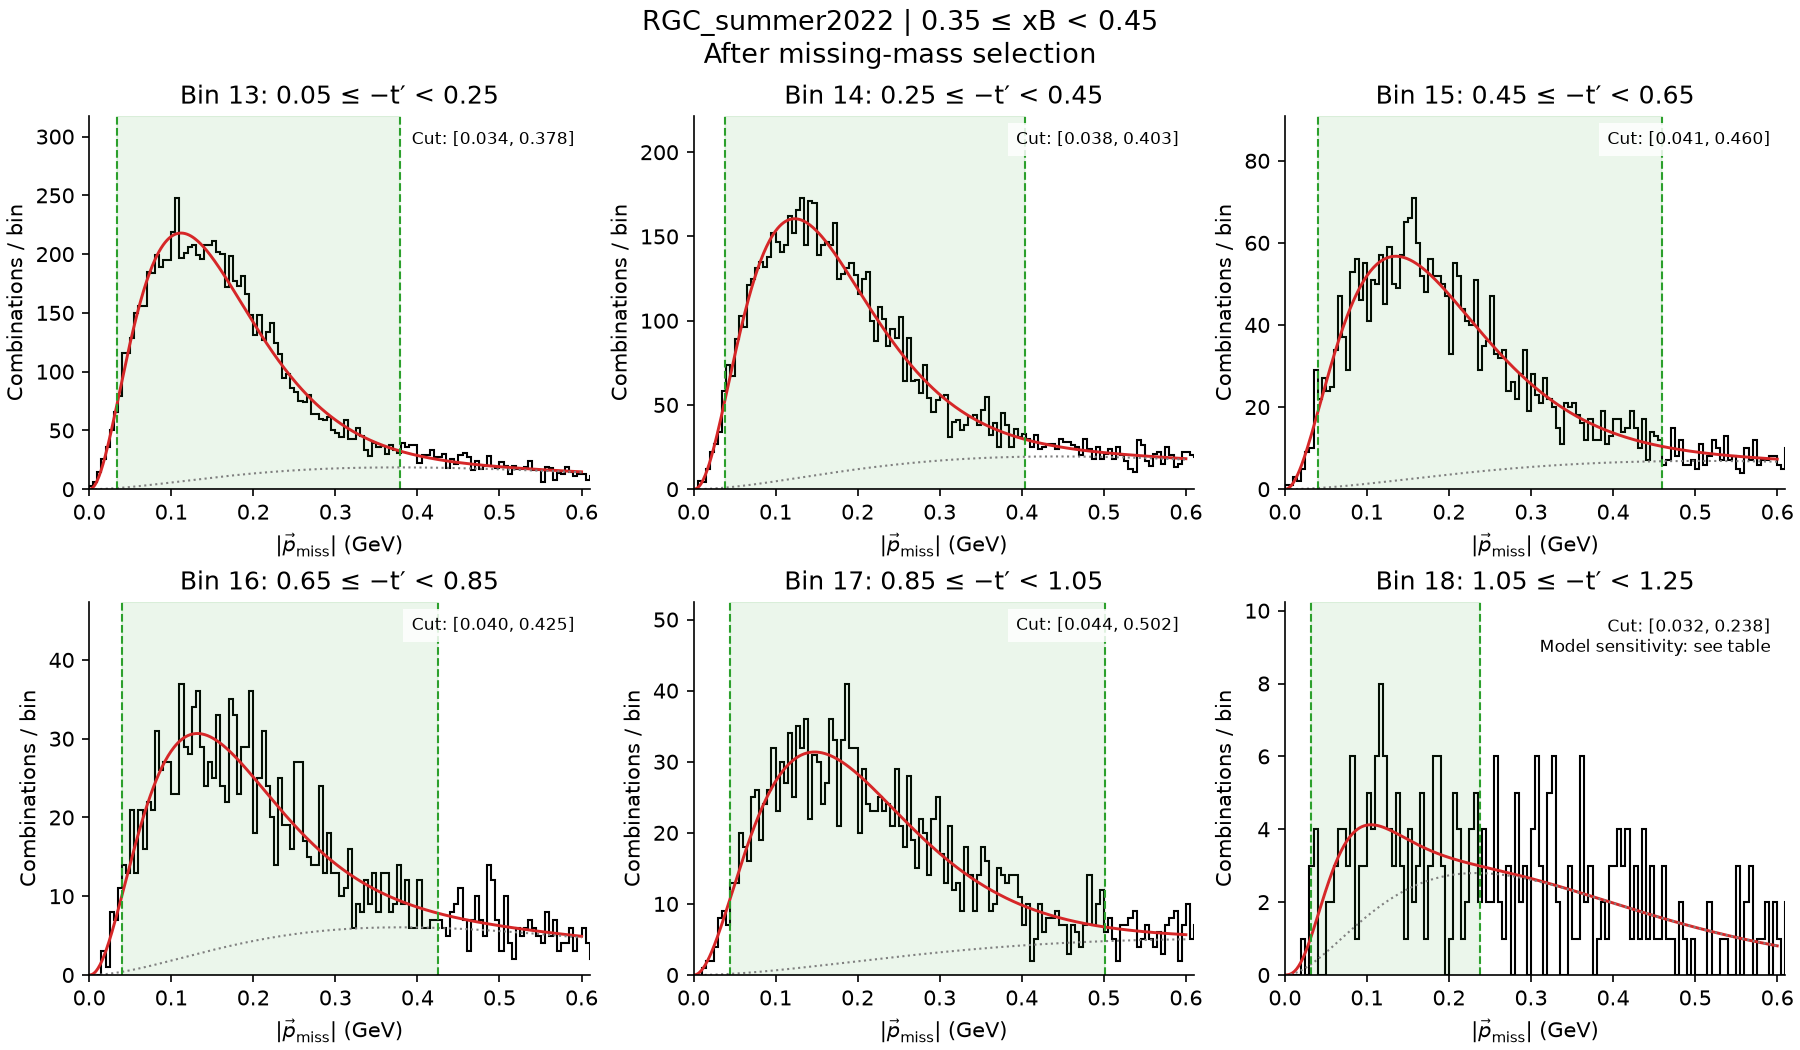
\includegraphics[width=\linewidth]{figures/channel_selection/exclusivity/rgc_su22_momentum_xb3.png}
\caption{RGC\_summer2022: missing-momentum fits after the mass cut in $x_B$ interval 3. The panels retain the six fine selection bins.}\label{fig:new_excl_rgc_su22_momentum3}
\end{figure}
\clearpage
\begin{figure}[p]\centering
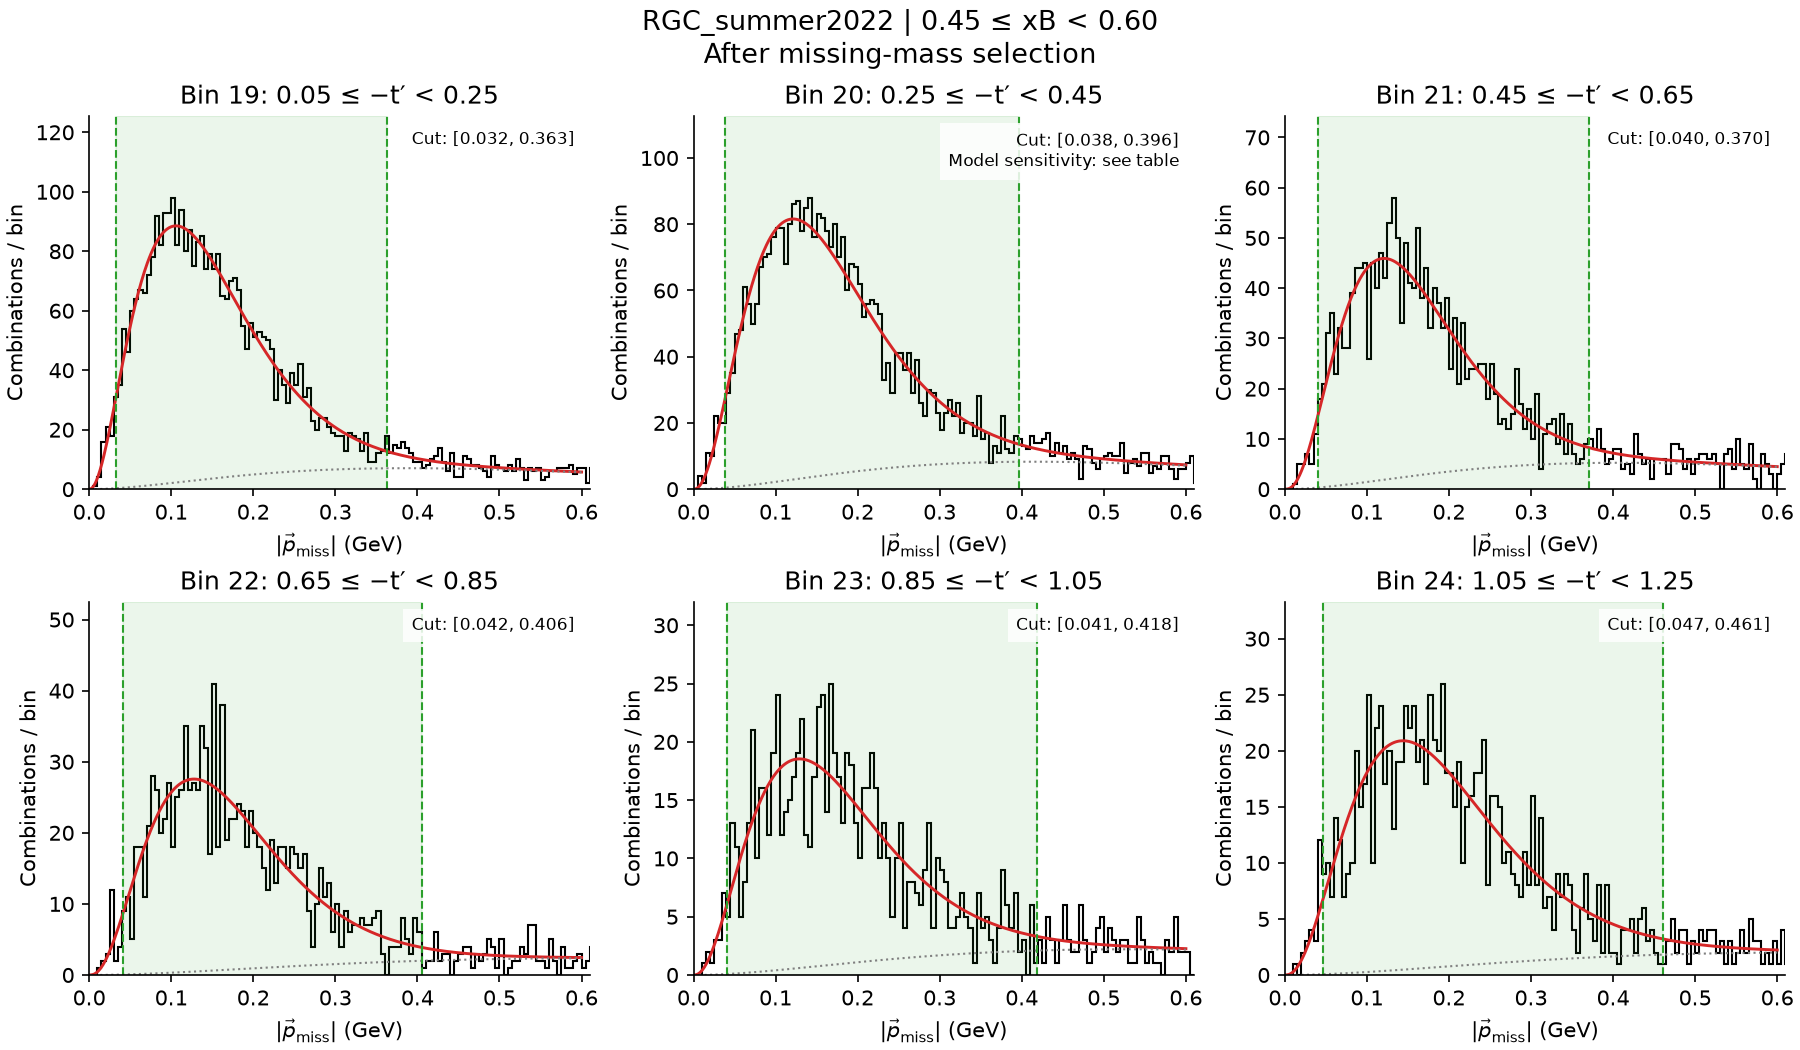
\includegraphics[width=\linewidth]{figures/channel_selection/exclusivity/rgc_su22_momentum_xb4.png}
\caption{RGC\_summer2022: missing-momentum fits after the mass cut in $x_B$ interval 4. The panels retain the six fine selection bins.}\label{fig:new_excl_rgc_su22_momentum4}
\end{figure}
\clearpage
\begin{figure}[p]\centering
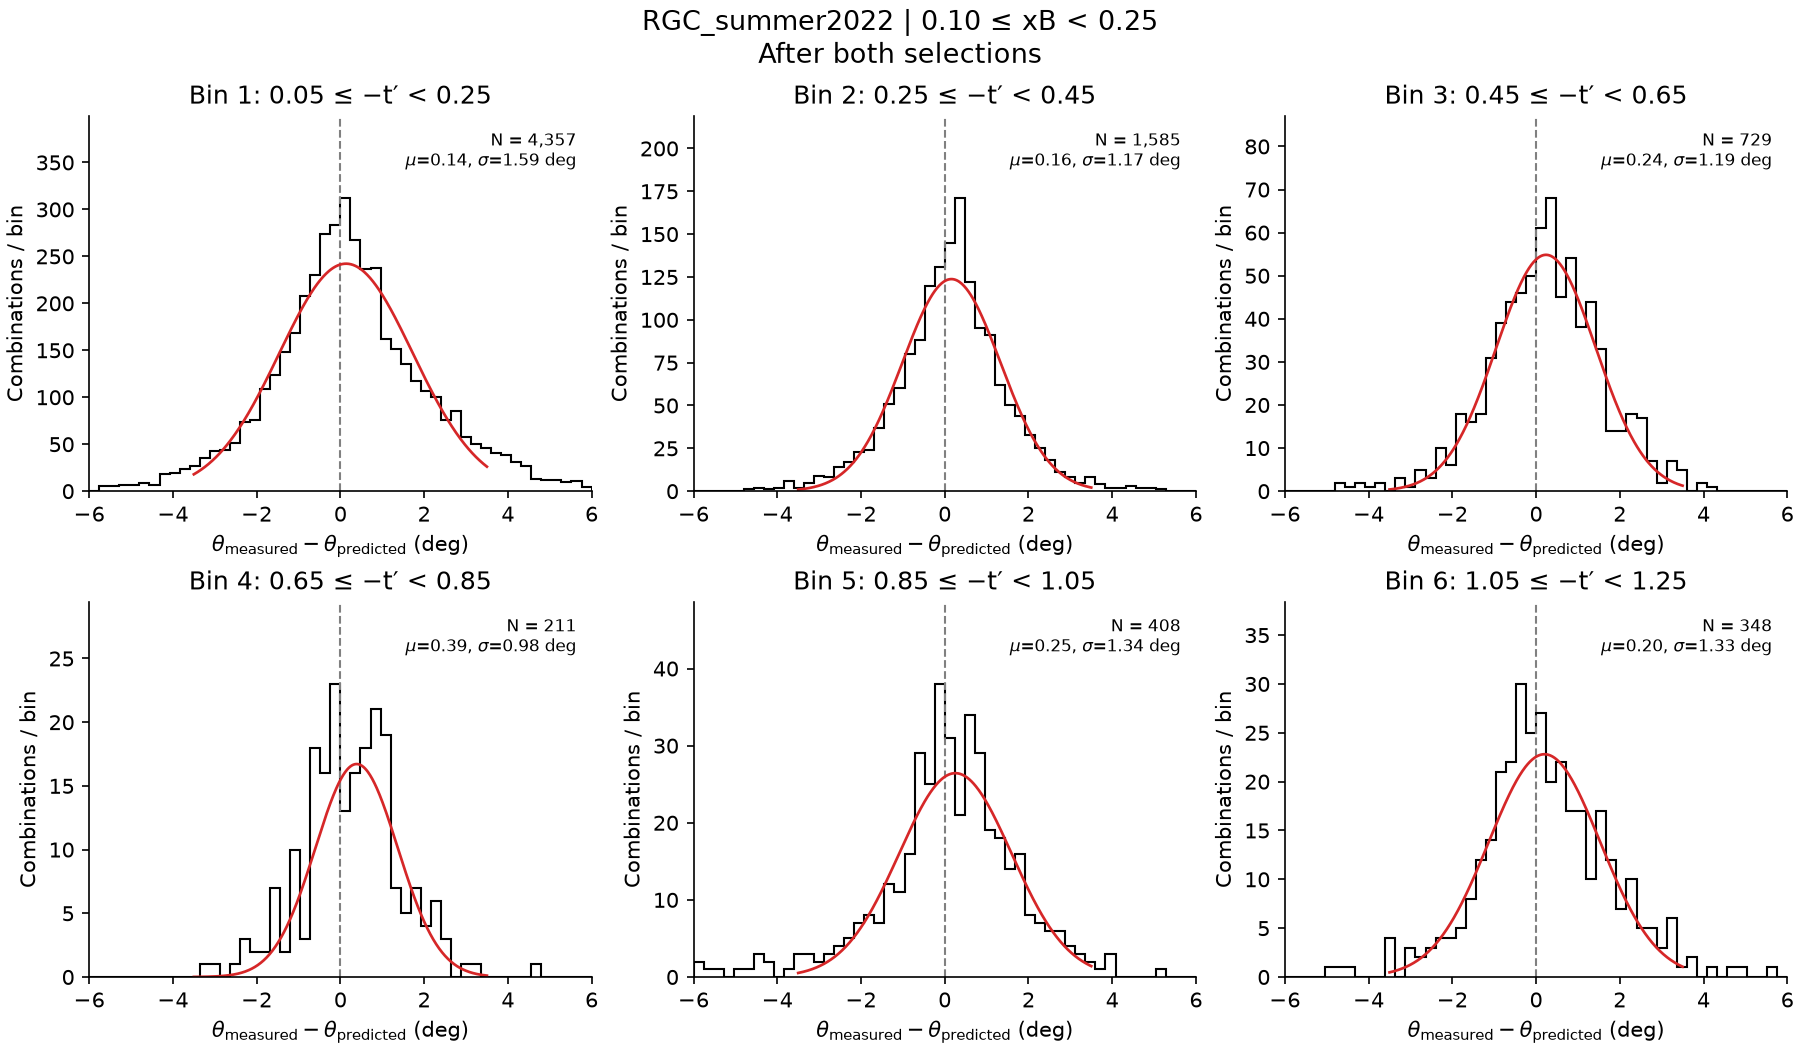
\includegraphics[width=\linewidth]{figures/channel_selection/exclusivity/rgc_su22_angle_xb1.png}
\caption{RGC\_summer2022: pion polar-angle closure after both cuts in $x_B$ interval 1. The panels retain the six fine selection bins.}\label{fig:new_excl_rgc_su22_angle1}
\end{figure}
\clearpage
\begin{figure}[p]\centering
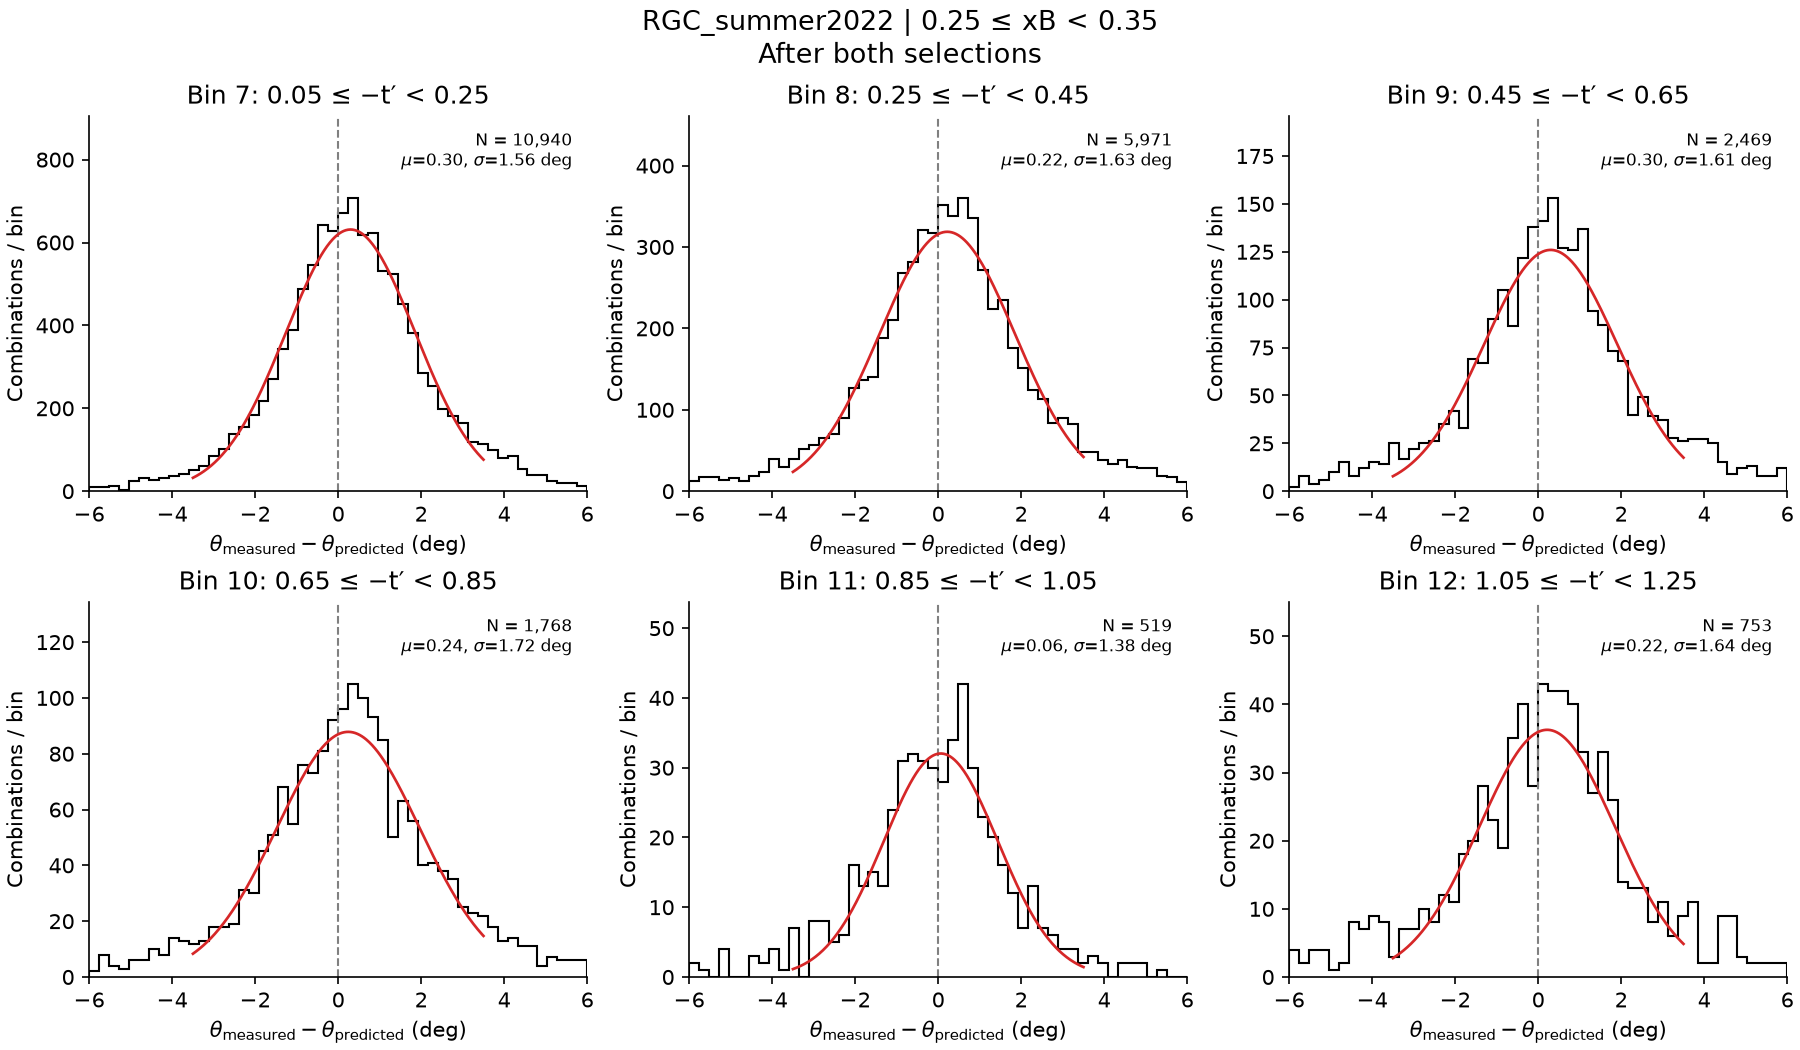
\includegraphics[width=\linewidth]{figures/channel_selection/exclusivity/rgc_su22_angle_xb2.png}
\caption{RGC\_summer2022: pion polar-angle closure after both cuts in $x_B$ interval 2. The panels retain the six fine selection bins.}\label{fig:new_excl_rgc_su22_angle2}
\end{figure}
\clearpage
\begin{figure}[p]\centering
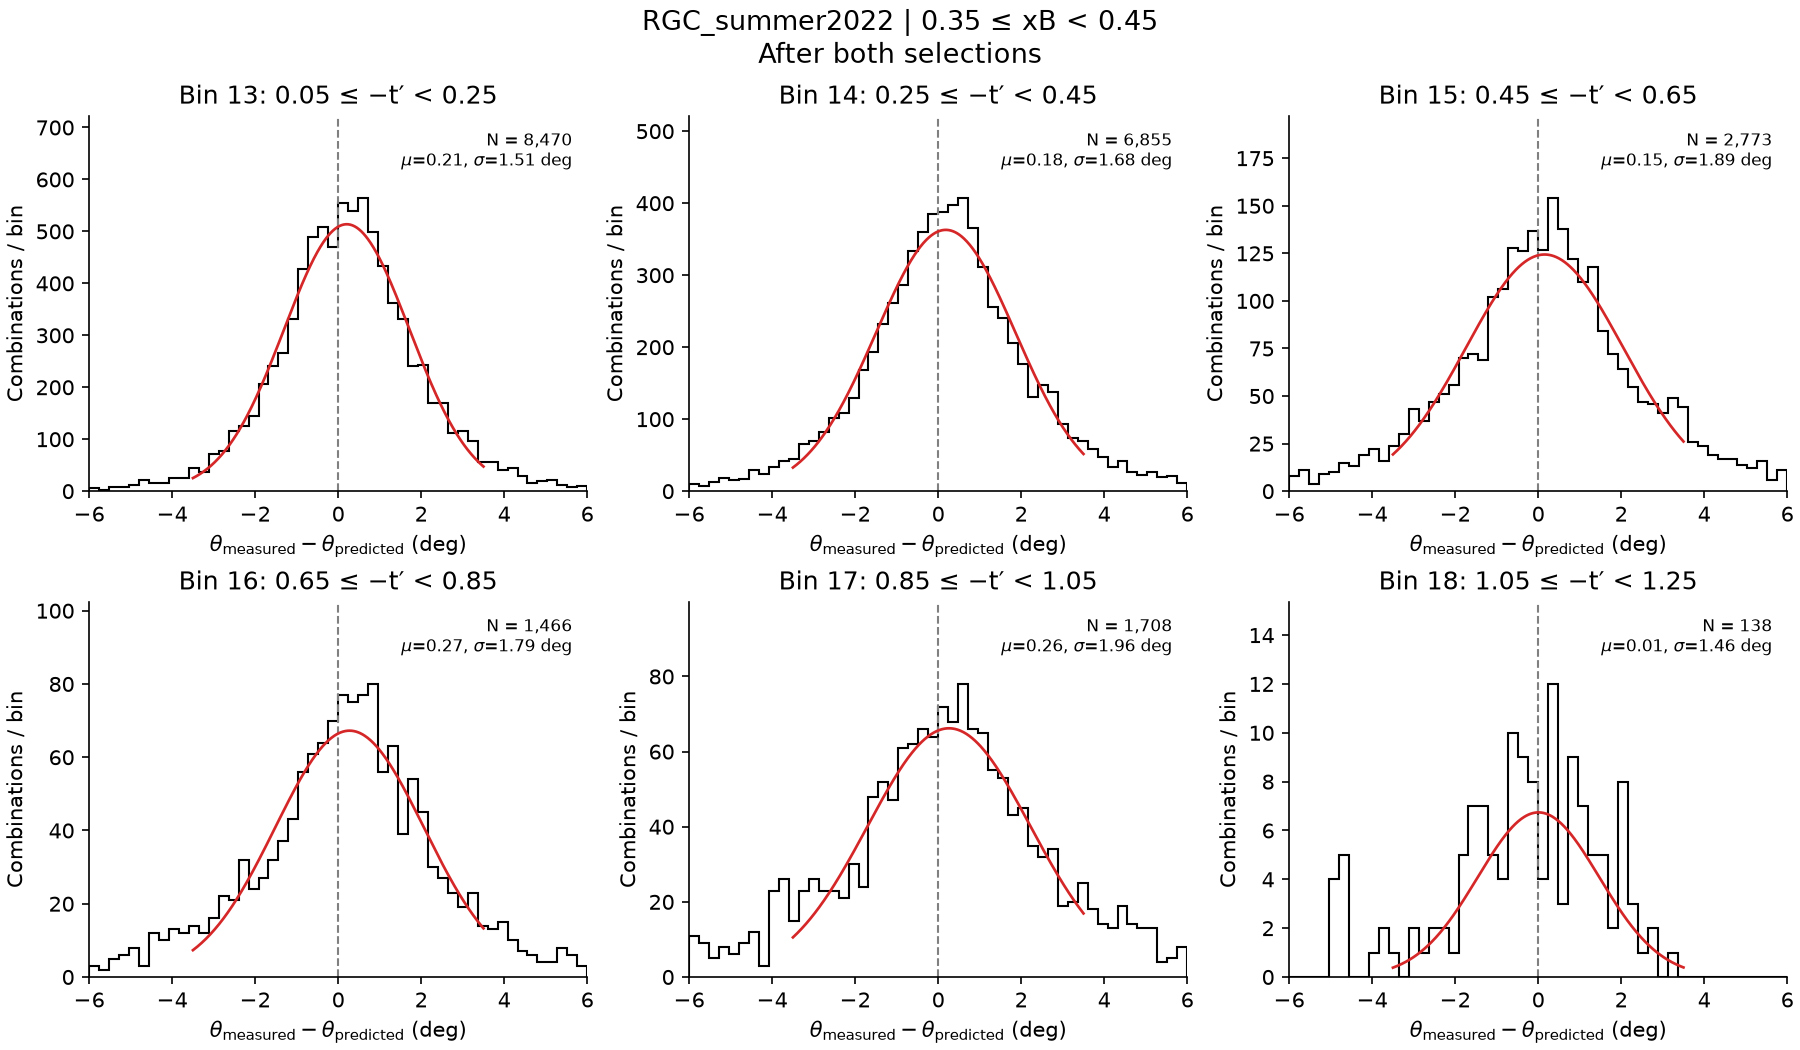
\includegraphics[width=\linewidth]{figures/channel_selection/exclusivity/rgc_su22_angle_xb3.png}
\caption{RGC\_summer2022: pion polar-angle closure after both cuts in $x_B$ interval 3. The panels retain the six fine selection bins.}\label{fig:new_excl_rgc_su22_angle3}
\end{figure}
\clearpage
\begin{figure}[p]\centering
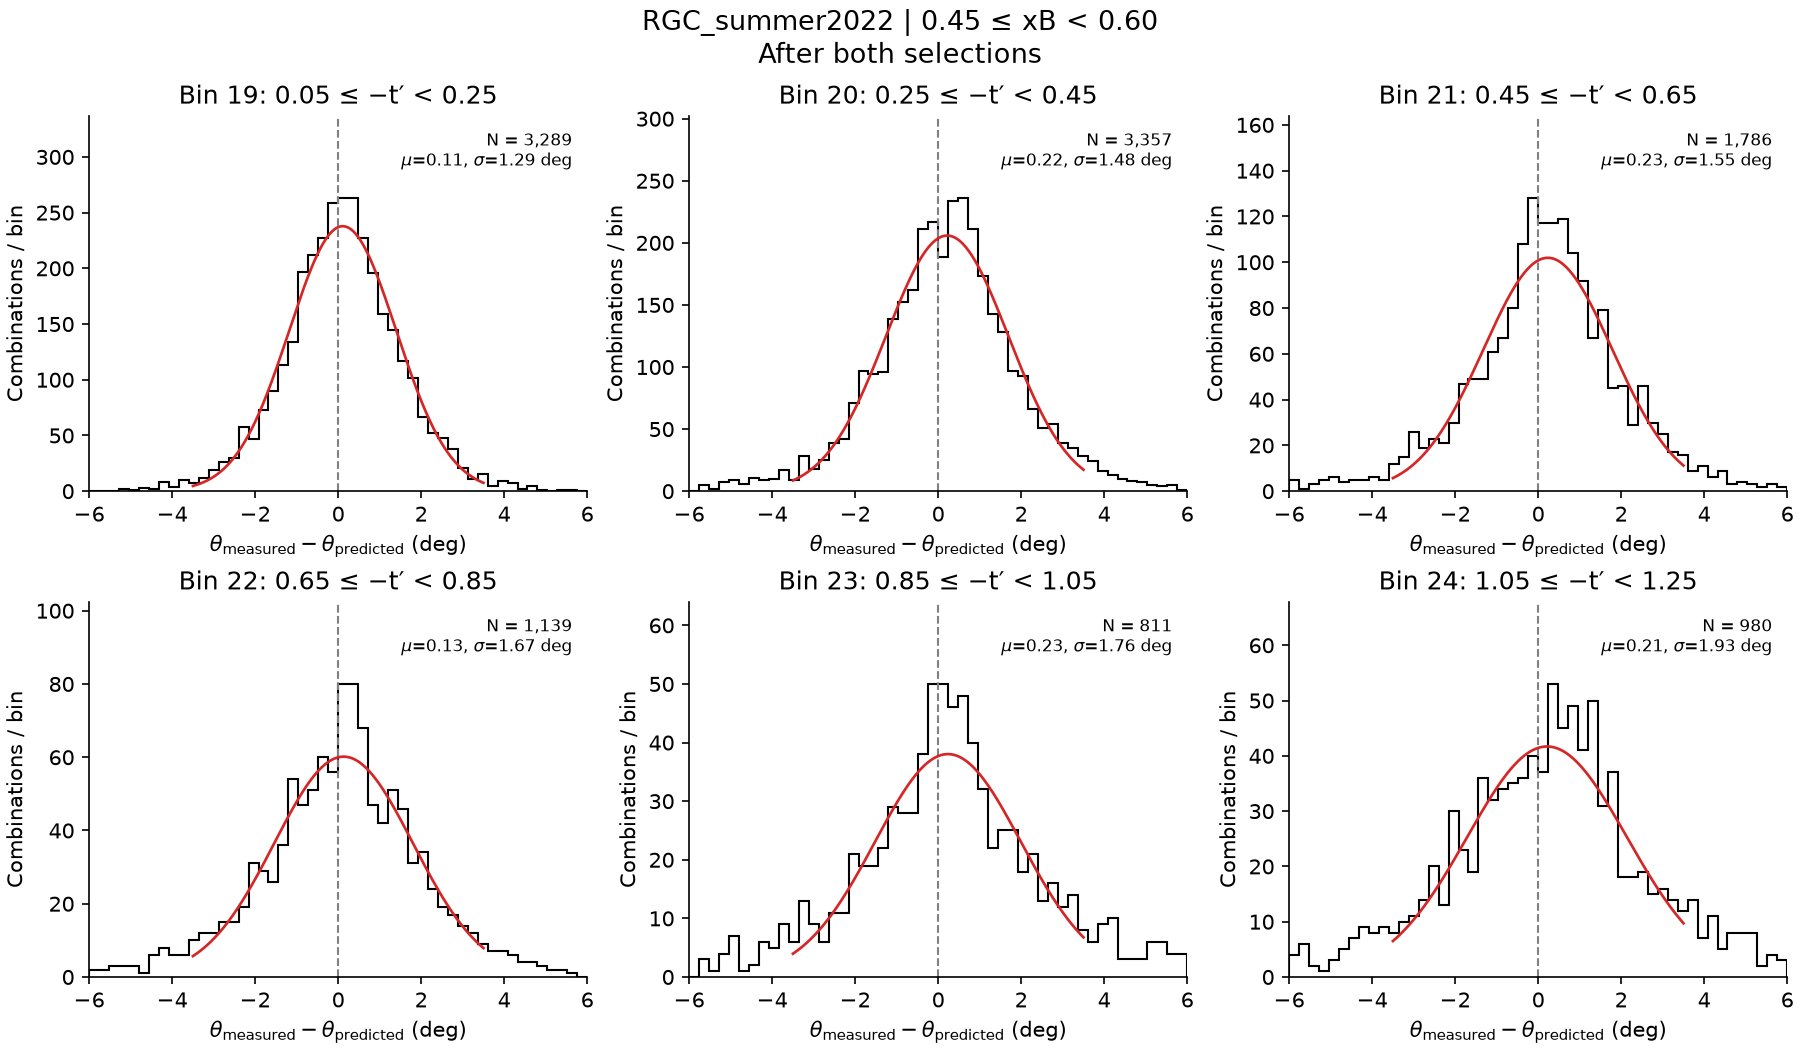
\includegraphics[width=\linewidth]{figures/channel_selection/exclusivity/rgc_su22_angle_xb4.png}
\caption{RGC\_summer2022: pion polar-angle closure after both cuts in $x_B$ interval 4. The panels retain the six fine selection bins.}\label{fig:new_excl_rgc_su22_angle4}
\end{figure}
\clearpage
\begin{figure}[p]\centering
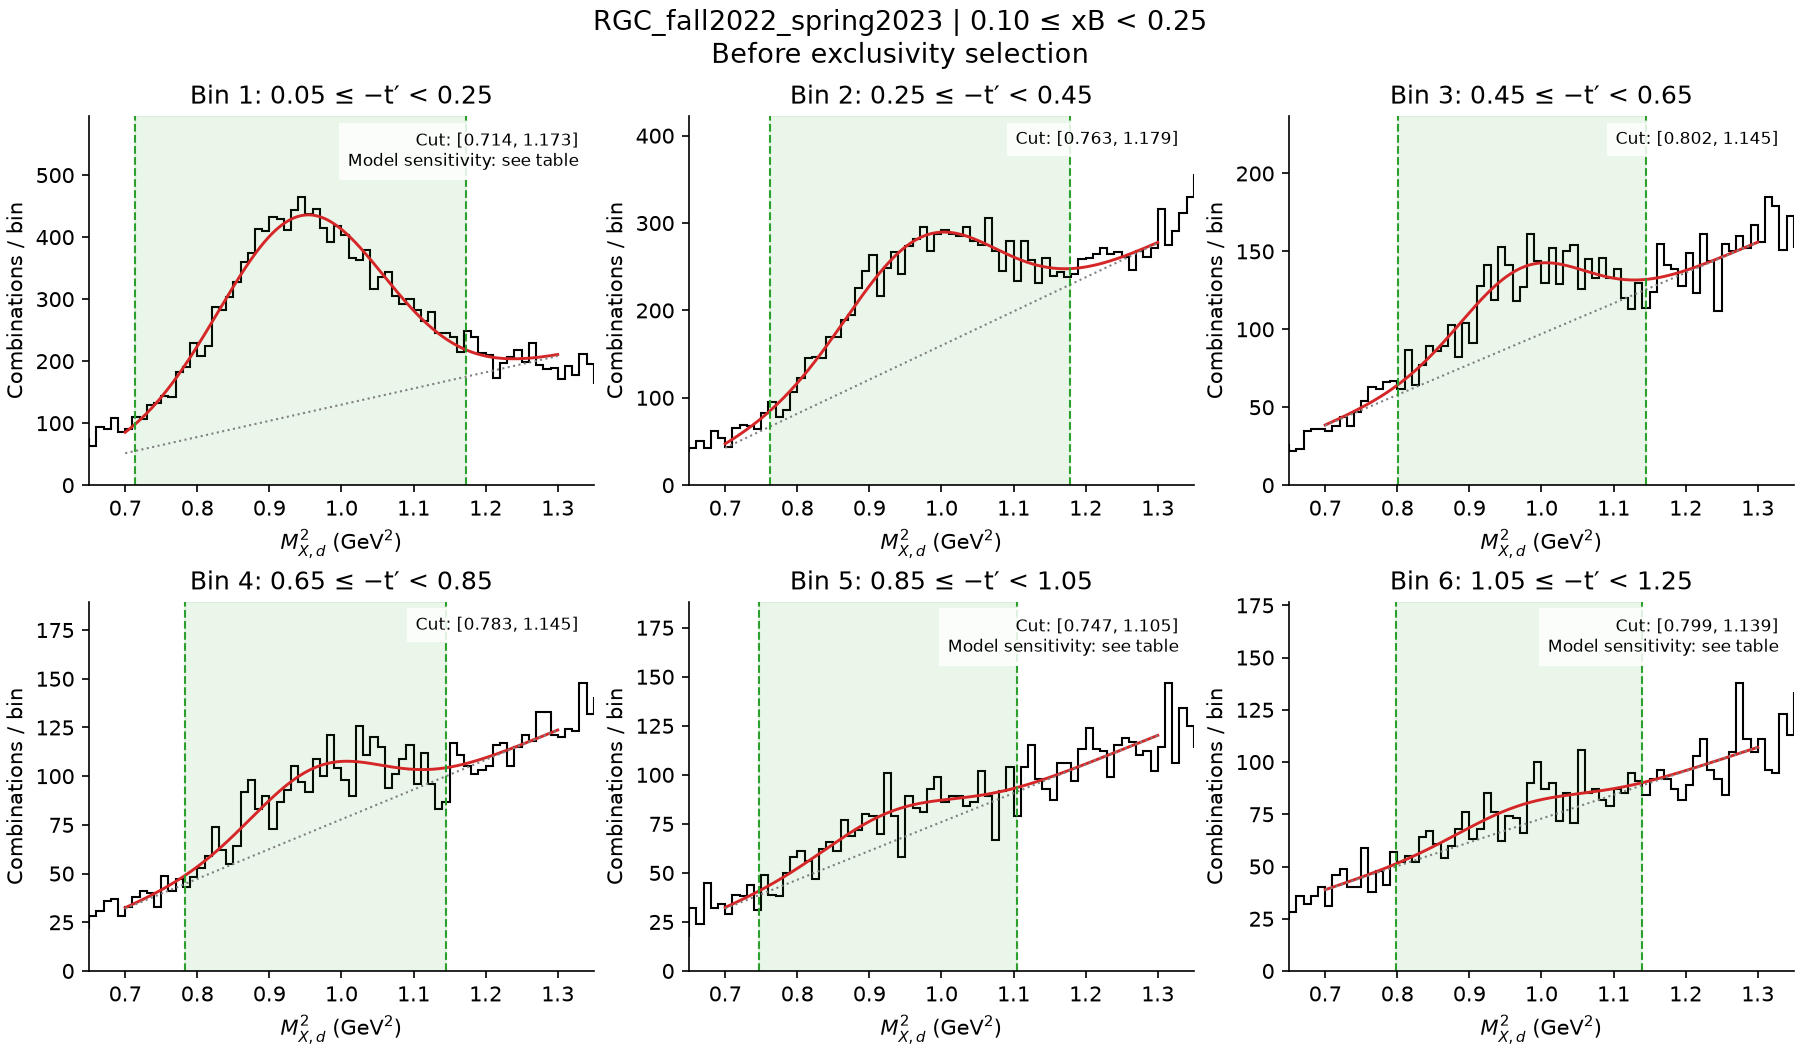
\includegraphics[width=\linewidth]{figures/channel_selection/exclusivity/rgc_fa22_sp23_mass_xb1.png}
\caption{RGC\_fall2022\_spring2023: deuteron-reference missing-mass-squared fits in $x_B$ interval 1. The panels retain the six fine selection bins.}\label{fig:new_excl_rgc_fa22_sp23_mass1}
\end{figure}
\clearpage
\begin{figure}[p]\centering
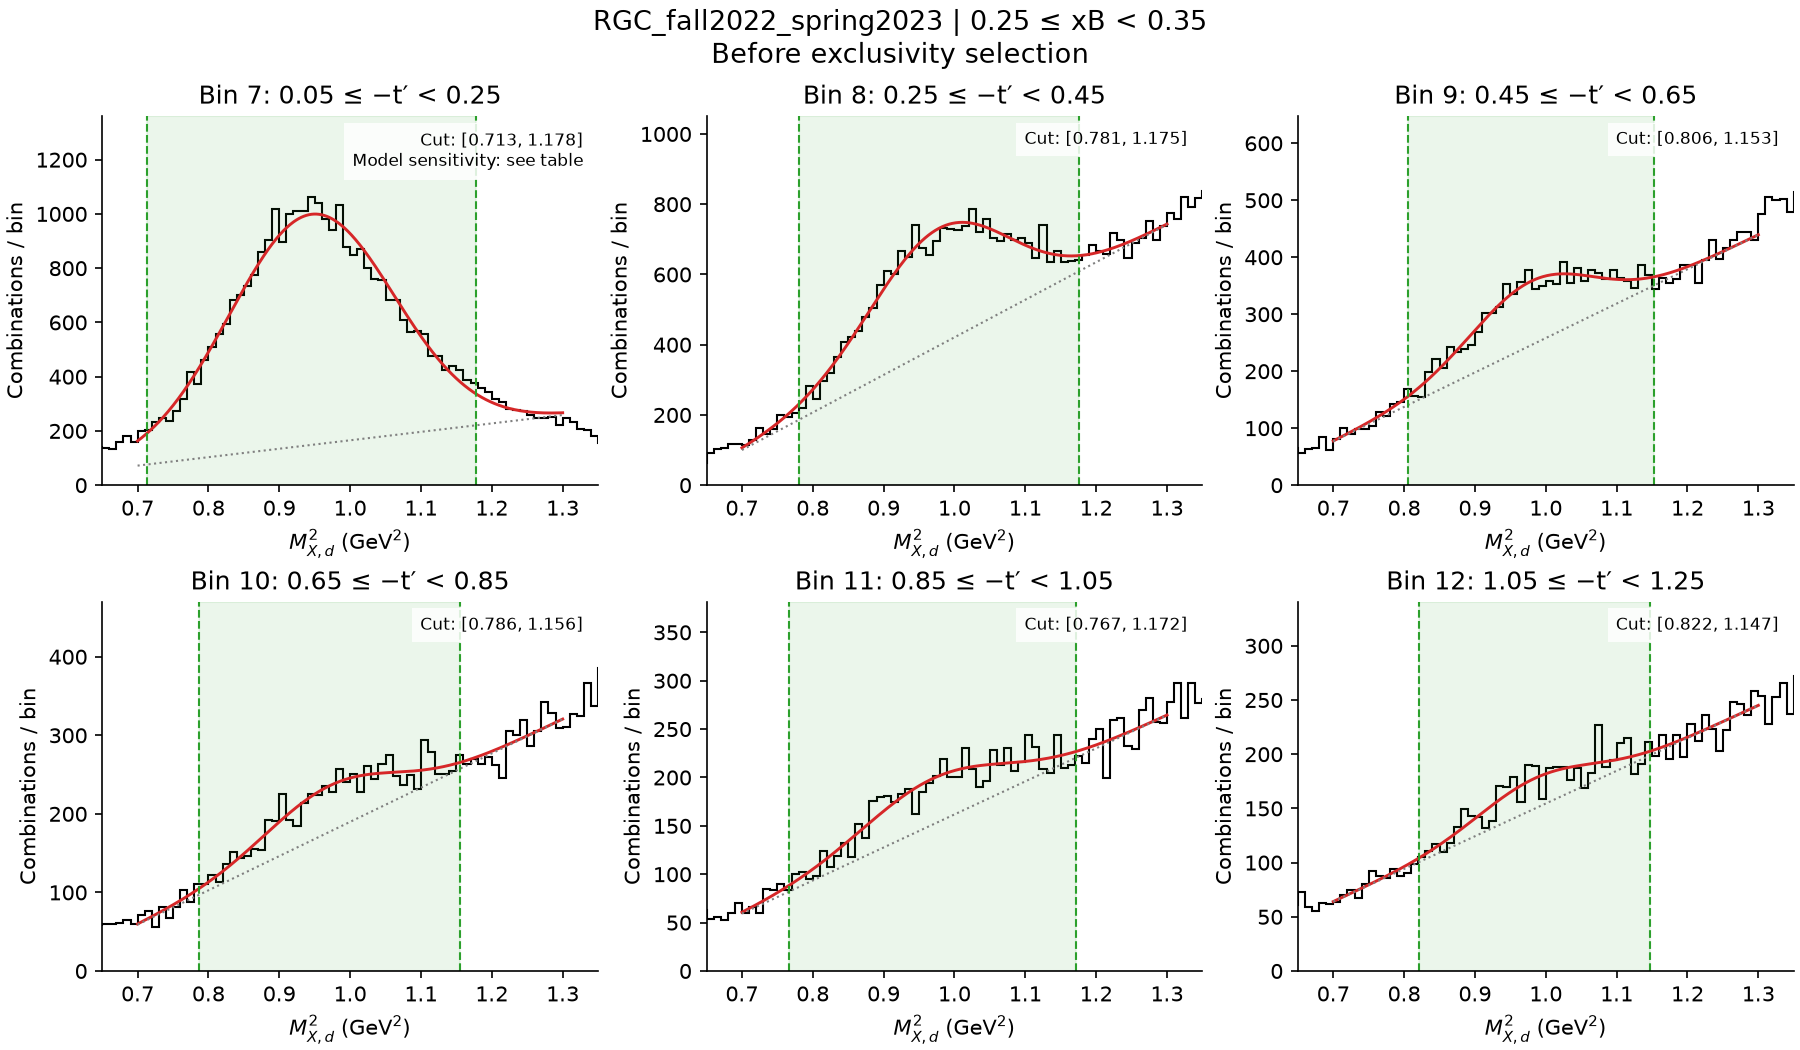
\includegraphics[width=\linewidth]{figures/channel_selection/exclusivity/rgc_fa22_sp23_mass_xb2.png}
\caption{RGC\_fall2022\_spring2023: deuteron-reference missing-mass-squared fits in $x_B$ interval 2. The panels retain the six fine selection bins.}\label{fig:new_excl_rgc_fa22_sp23_mass2}
\end{figure}
\clearpage
\begin{figure}[p]\centering
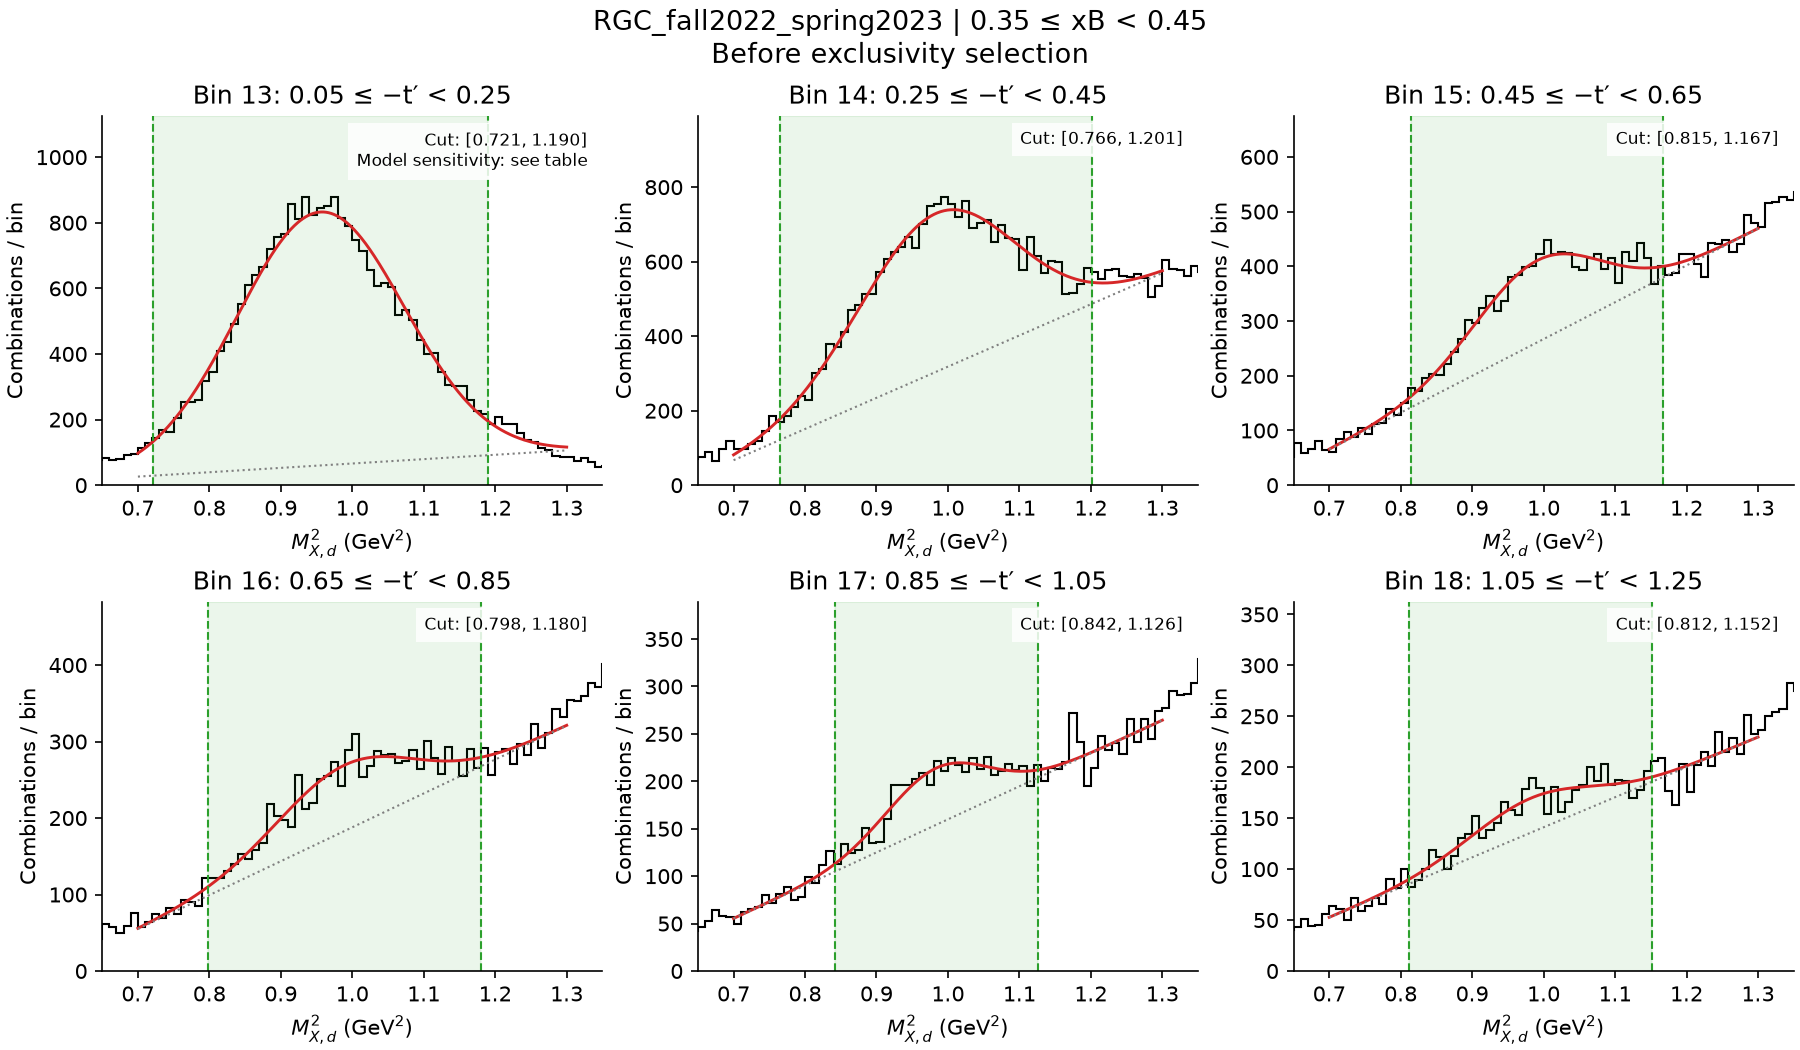
\includegraphics[width=\linewidth]{figures/channel_selection/exclusivity/rgc_fa22_sp23_mass_xb3.png}
\caption{RGC\_fall2022\_spring2023: deuteron-reference missing-mass-squared fits in $x_B$ interval 3. The panels retain the six fine selection bins.}\label{fig:new_excl_rgc_fa22_sp23_mass3}
\end{figure}
\clearpage
\begin{figure}[p]\centering
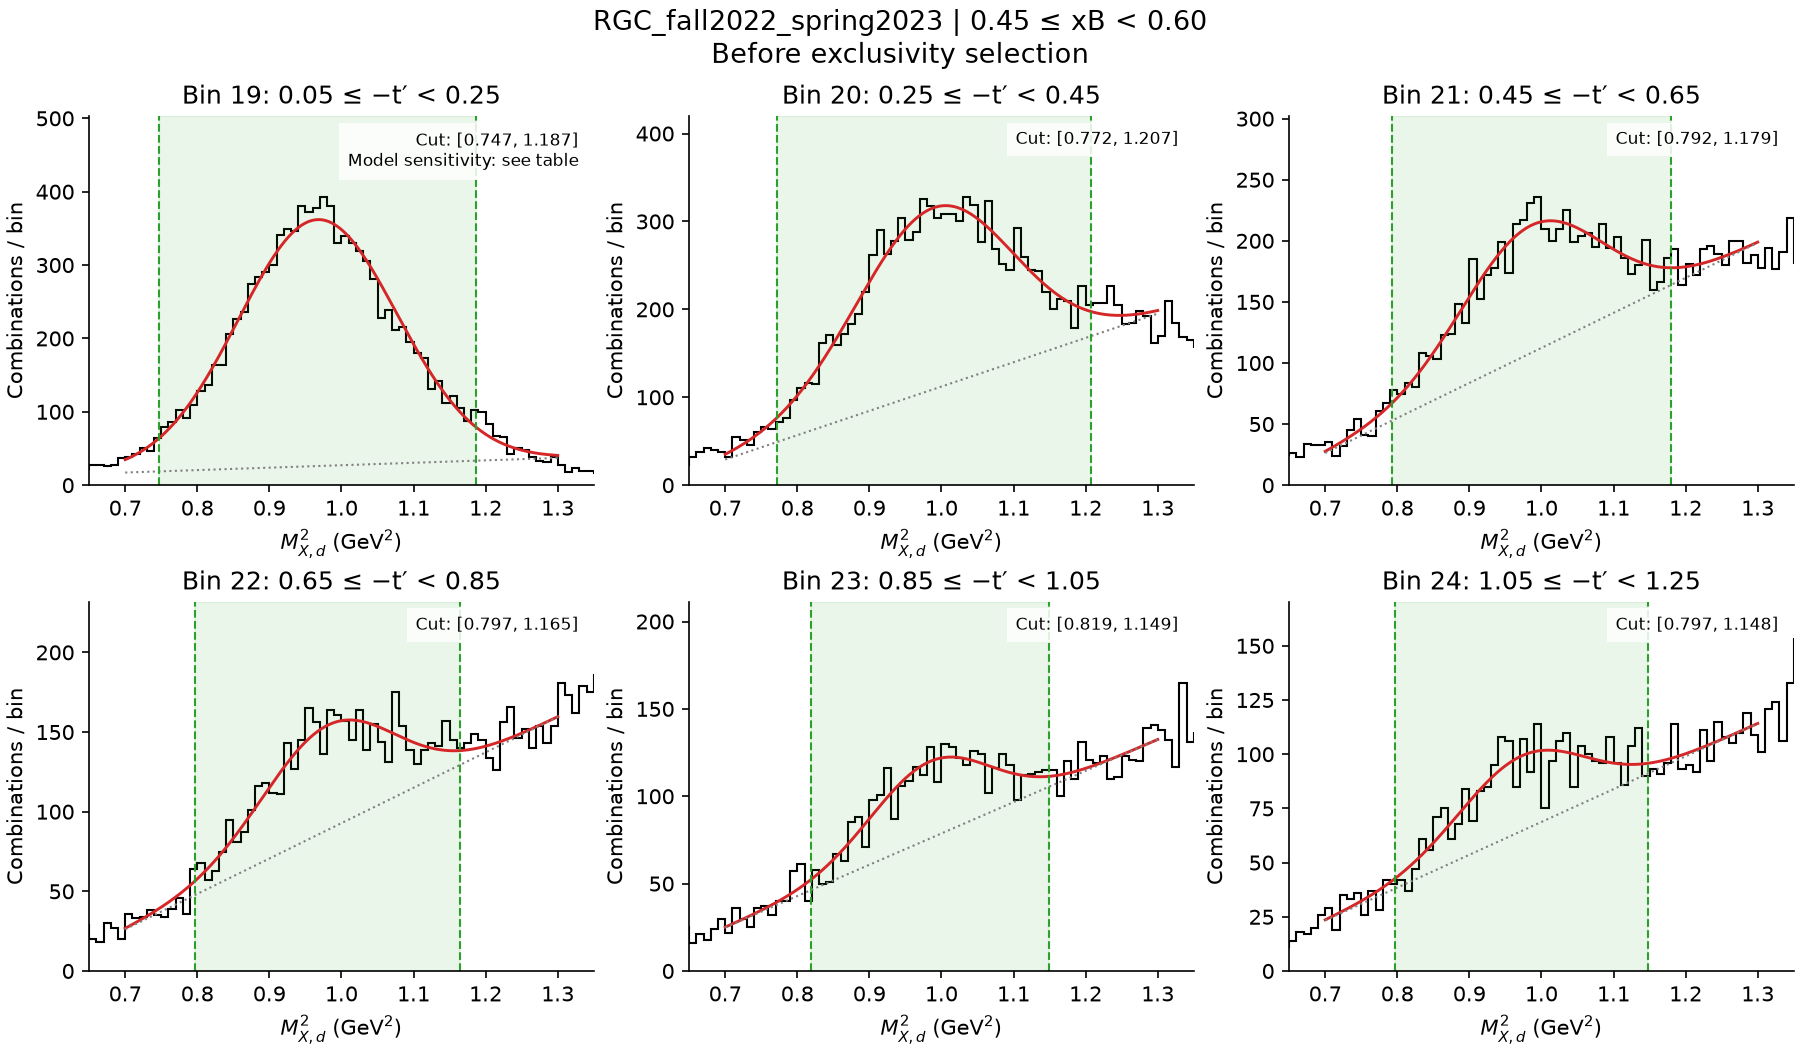
\includegraphics[width=\linewidth]{figures/channel_selection/exclusivity/rgc_fa22_sp23_mass_xb4.png}
\caption{RGC\_fall2022\_spring2023: deuteron-reference missing-mass-squared fits in $x_B$ interval 4. The panels retain the six fine selection bins.}\label{fig:new_excl_rgc_fa22_sp23_mass4}
\end{figure}
\clearpage
\begin{figure}[p]\centering
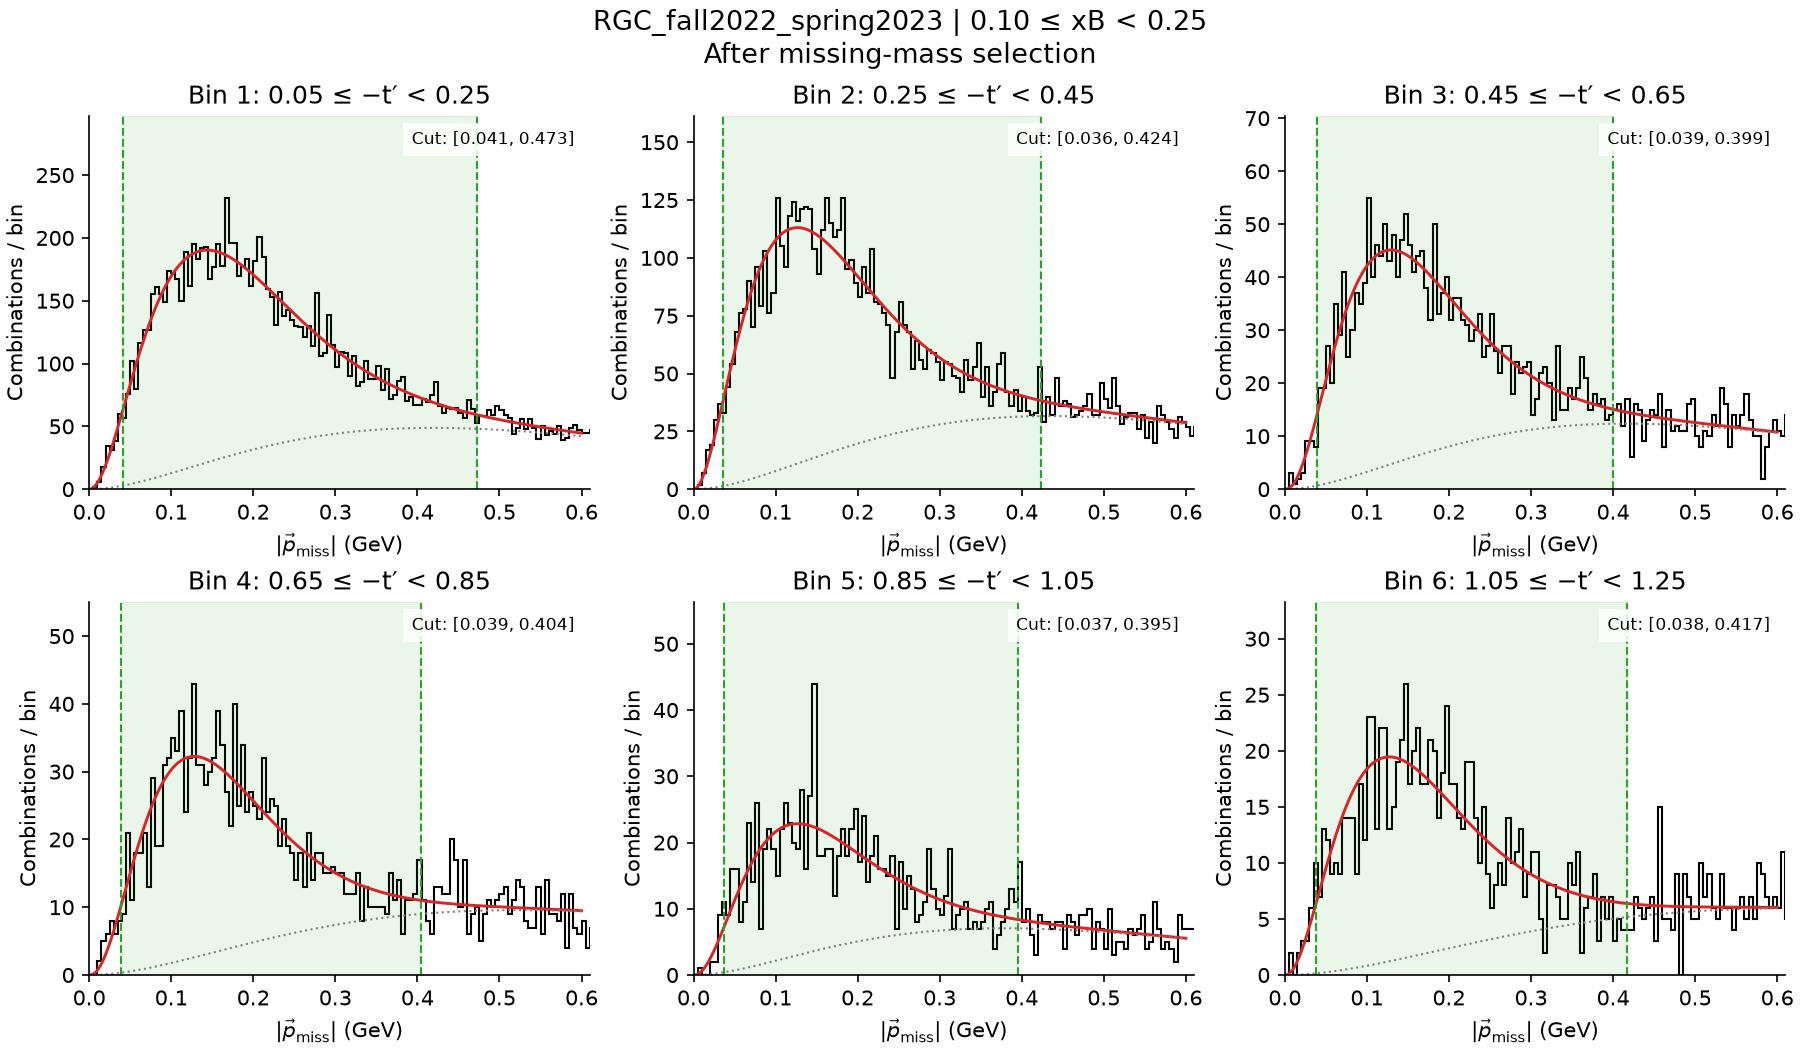
\includegraphics[width=\linewidth]{figures/channel_selection/exclusivity/rgc_fa22_sp23_momentum_xb1.png}
\caption{RGC\_fall2022\_spring2023: missing-momentum fits after the mass cut in $x_B$ interval 1. The panels retain the six fine selection bins.}\label{fig:new_excl_rgc_fa22_sp23_momentum1}
\end{figure}
\clearpage
\begin{figure}[p]\centering
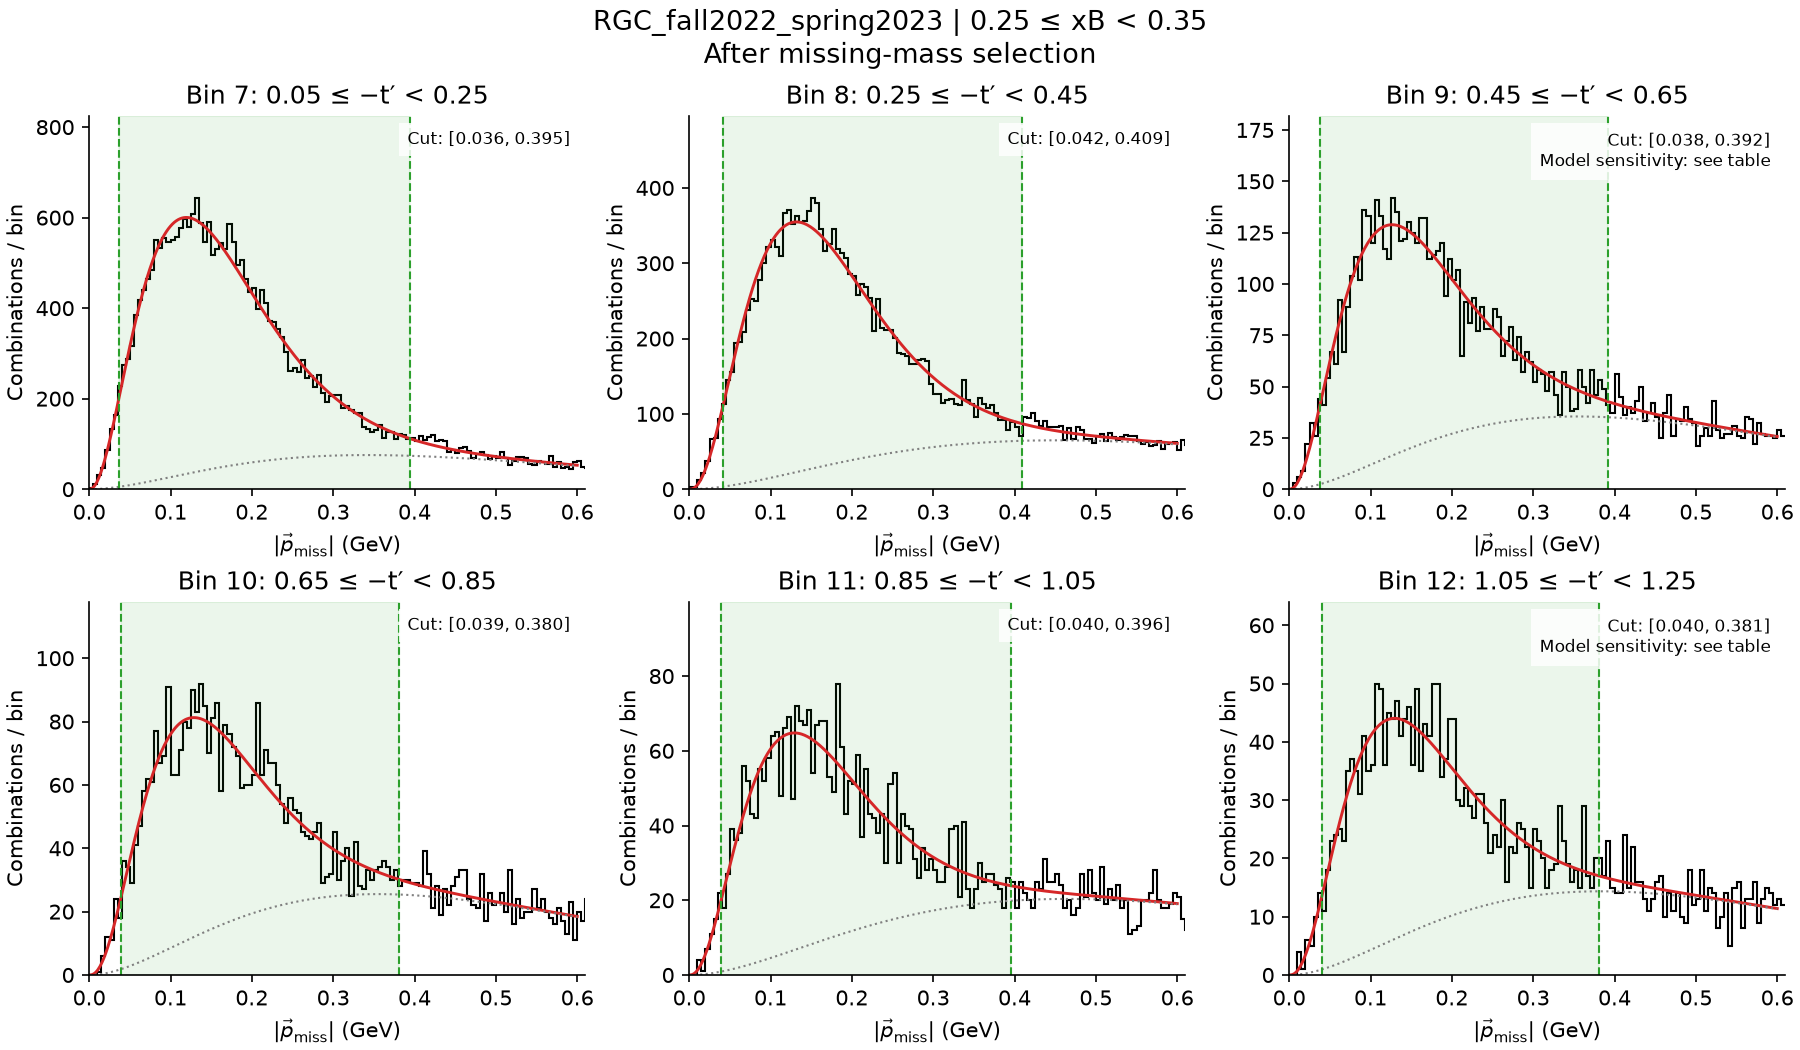
\includegraphics[width=\linewidth]{figures/channel_selection/exclusivity/rgc_fa22_sp23_momentum_xb2.png}
\caption{RGC\_fall2022\_spring2023: missing-momentum fits after the mass cut in $x_B$ interval 2. The panels retain the six fine selection bins.}\label{fig:new_excl_rgc_fa22_sp23_momentum2}
\end{figure}
\clearpage
\begin{figure}[p]\centering
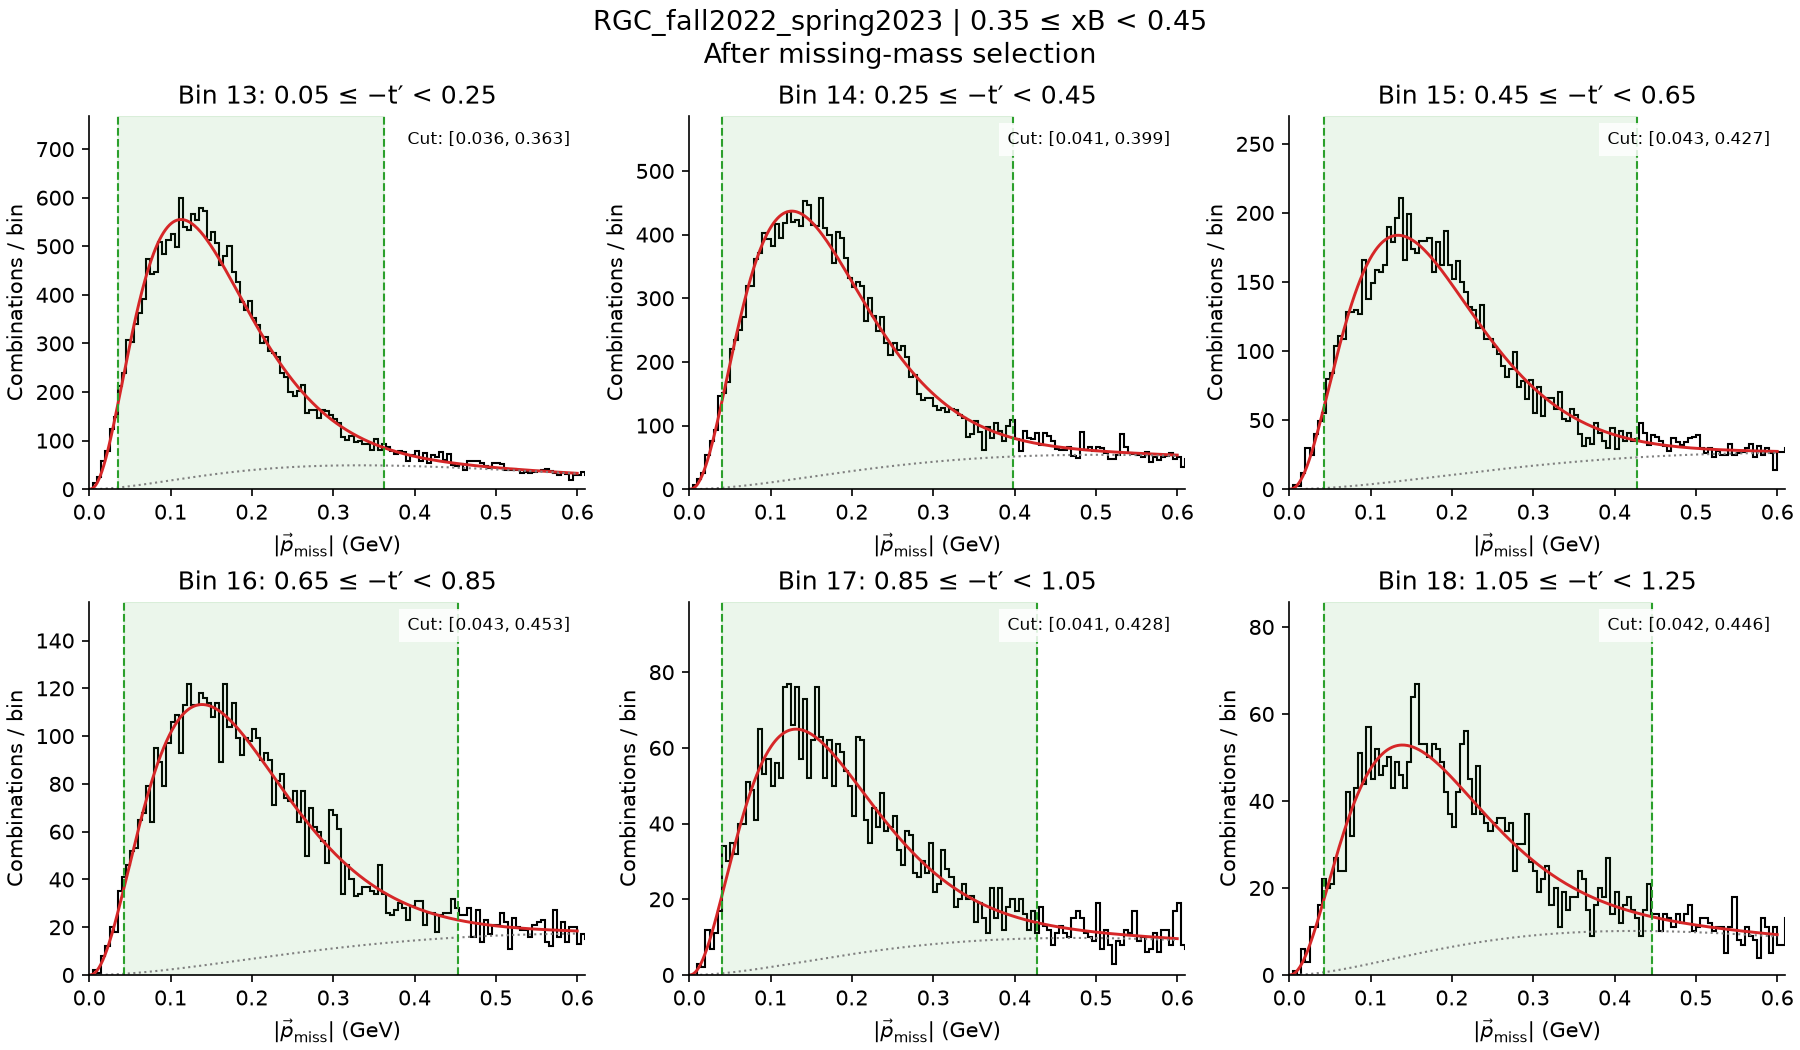
\includegraphics[width=\linewidth]{figures/channel_selection/exclusivity/rgc_fa22_sp23_momentum_xb3.png}
\caption{RGC\_fall2022\_spring2023: missing-momentum fits after the mass cut in $x_B$ interval 3. The panels retain the six fine selection bins.}\label{fig:new_excl_rgc_fa22_sp23_momentum3}
\end{figure}
\clearpage
\begin{figure}[p]\centering
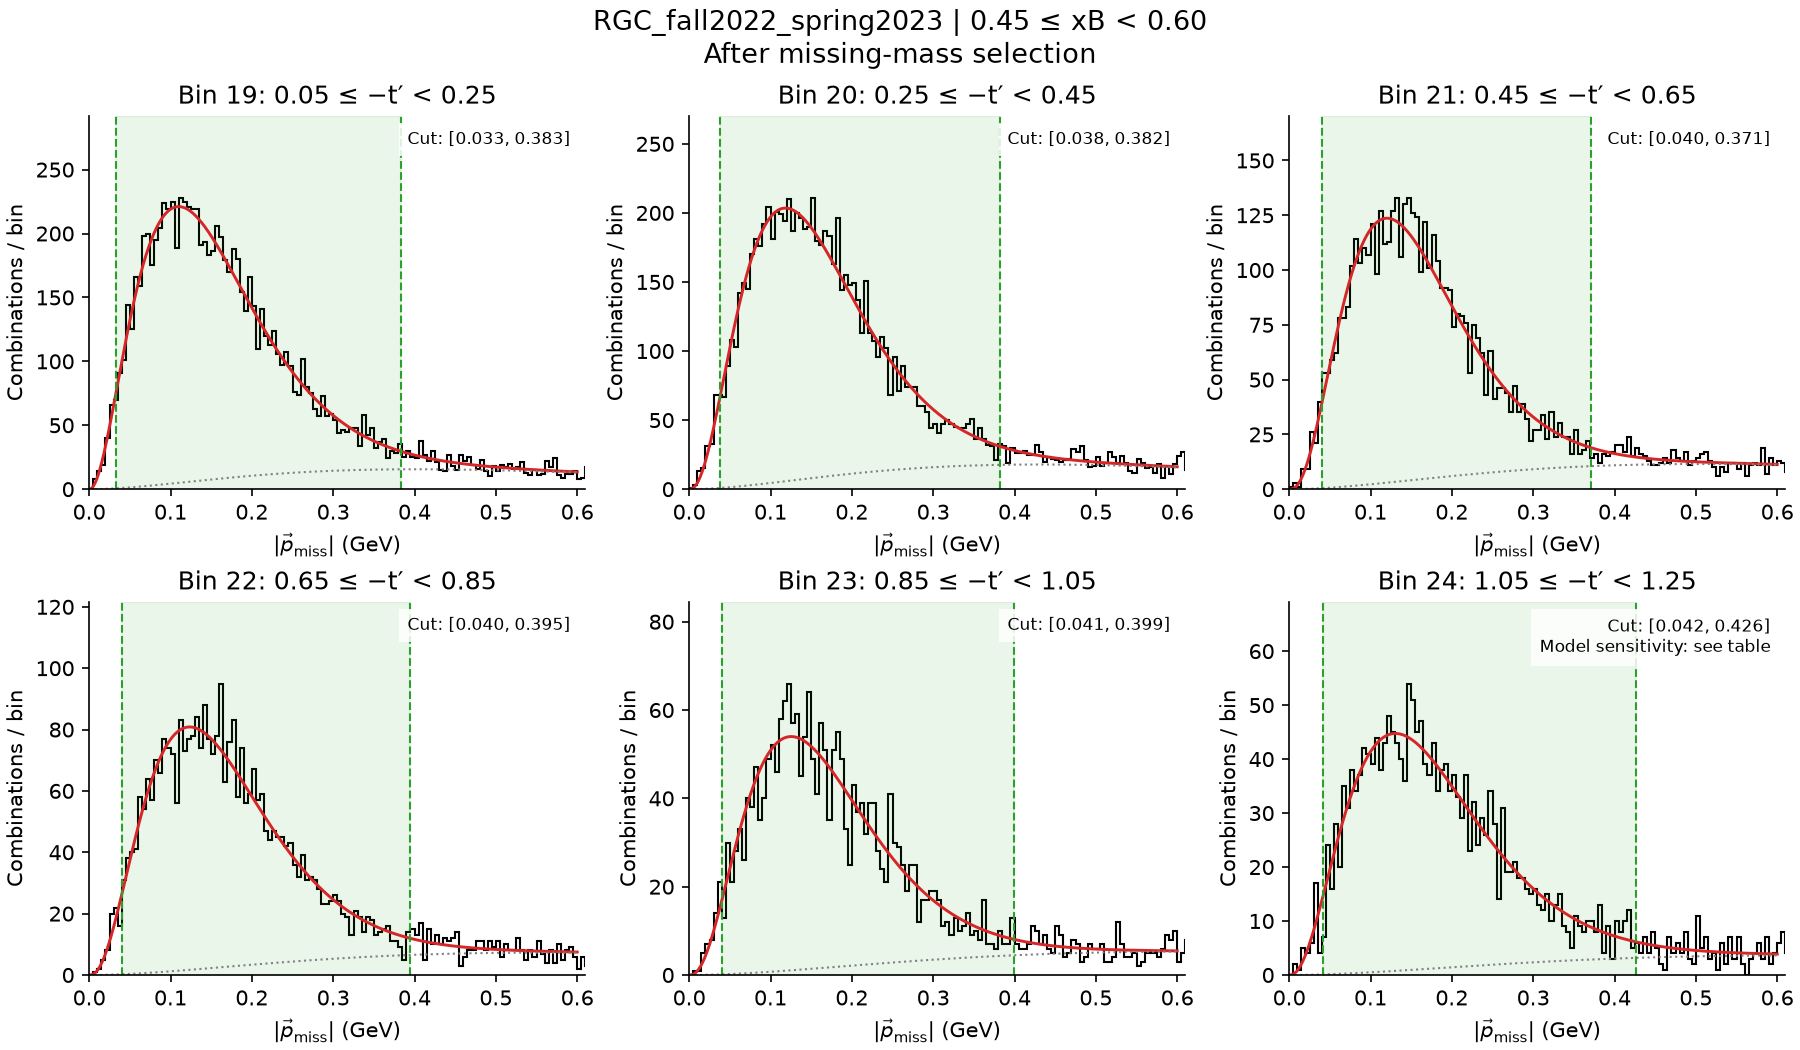
\includegraphics[width=\linewidth]{figures/channel_selection/exclusivity/rgc_fa22_sp23_momentum_xb4.png}
\caption{RGC\_fall2022\_spring2023: missing-momentum fits after the mass cut in $x_B$ interval 4. The panels retain the six fine selection bins.}\label{fig:new_excl_rgc_fa22_sp23_momentum4}
\end{figure}
\clearpage
\begin{figure}[p]\centering
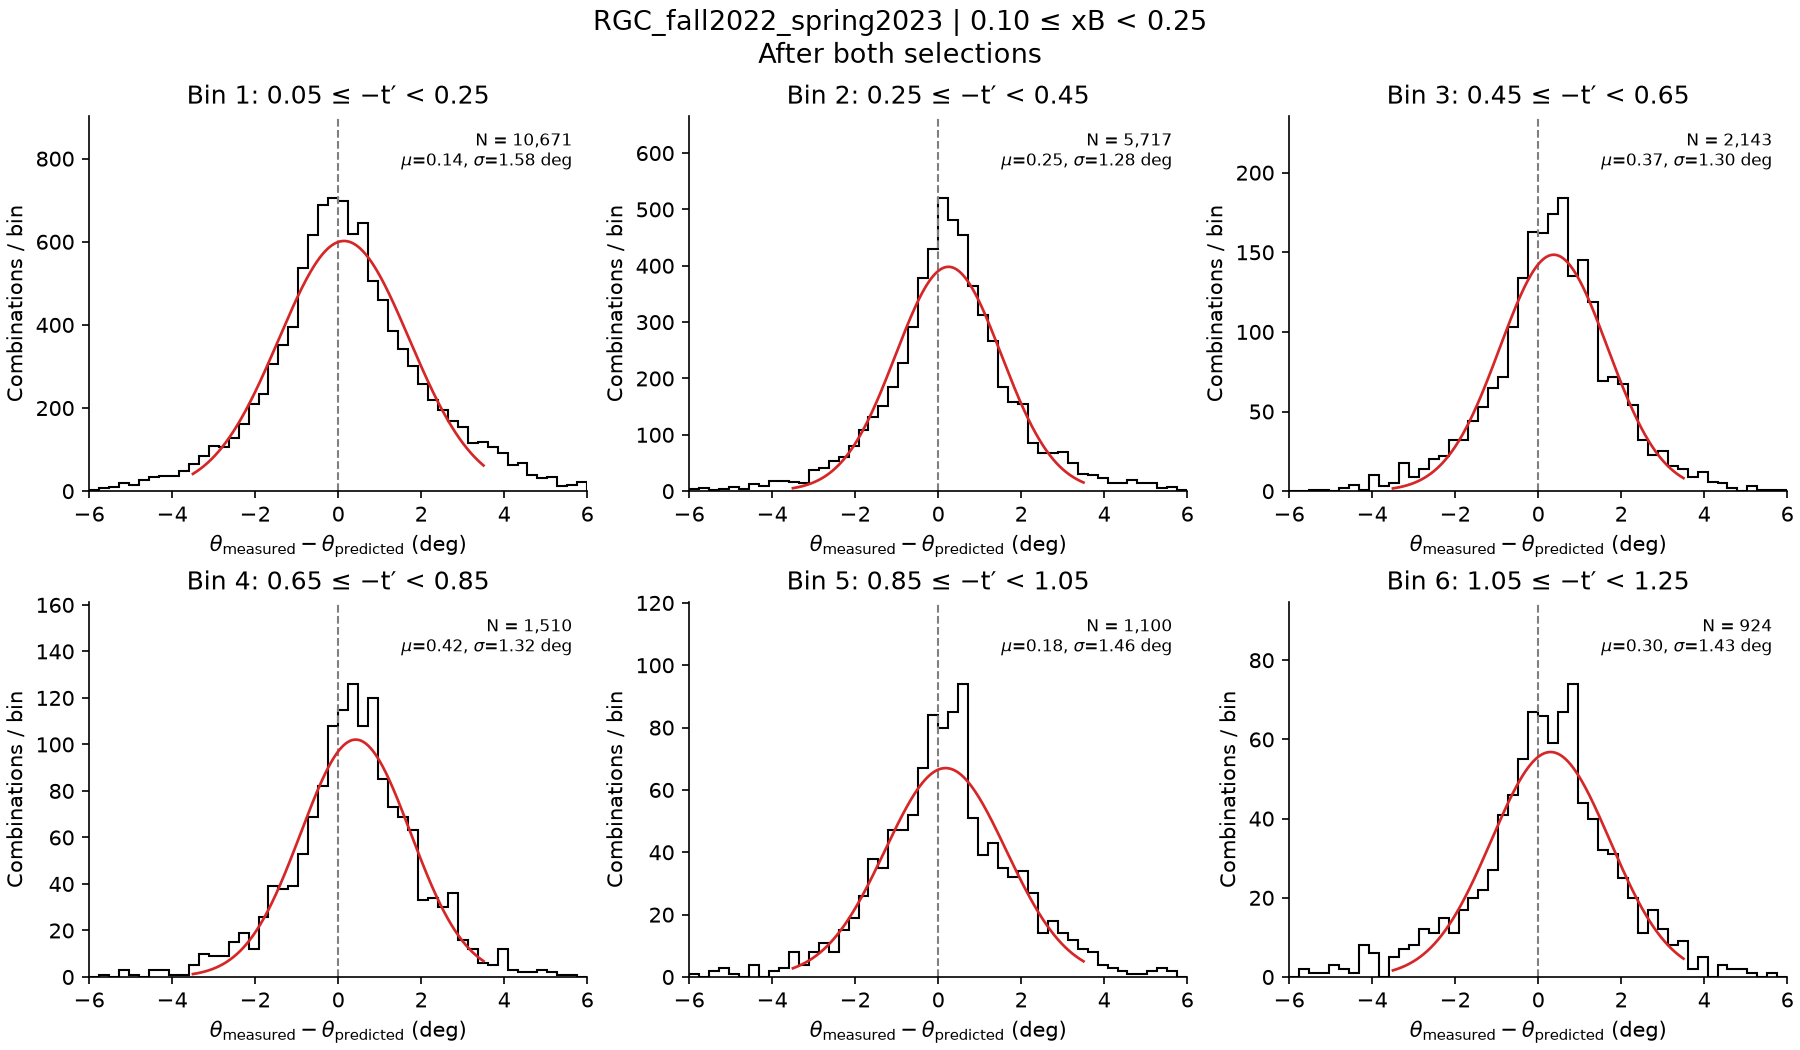
\includegraphics[width=\linewidth]{figures/channel_selection/exclusivity/rgc_fa22_sp23_angle_xb1.png}
\caption{RGC\_fall2022\_spring2023: pion polar-angle closure after both cuts in $x_B$ interval 1. The panels retain the six fine selection bins.}\label{fig:new_excl_rgc_fa22_sp23_angle1}
\end{figure}
\clearpage
\begin{figure}[p]\centering
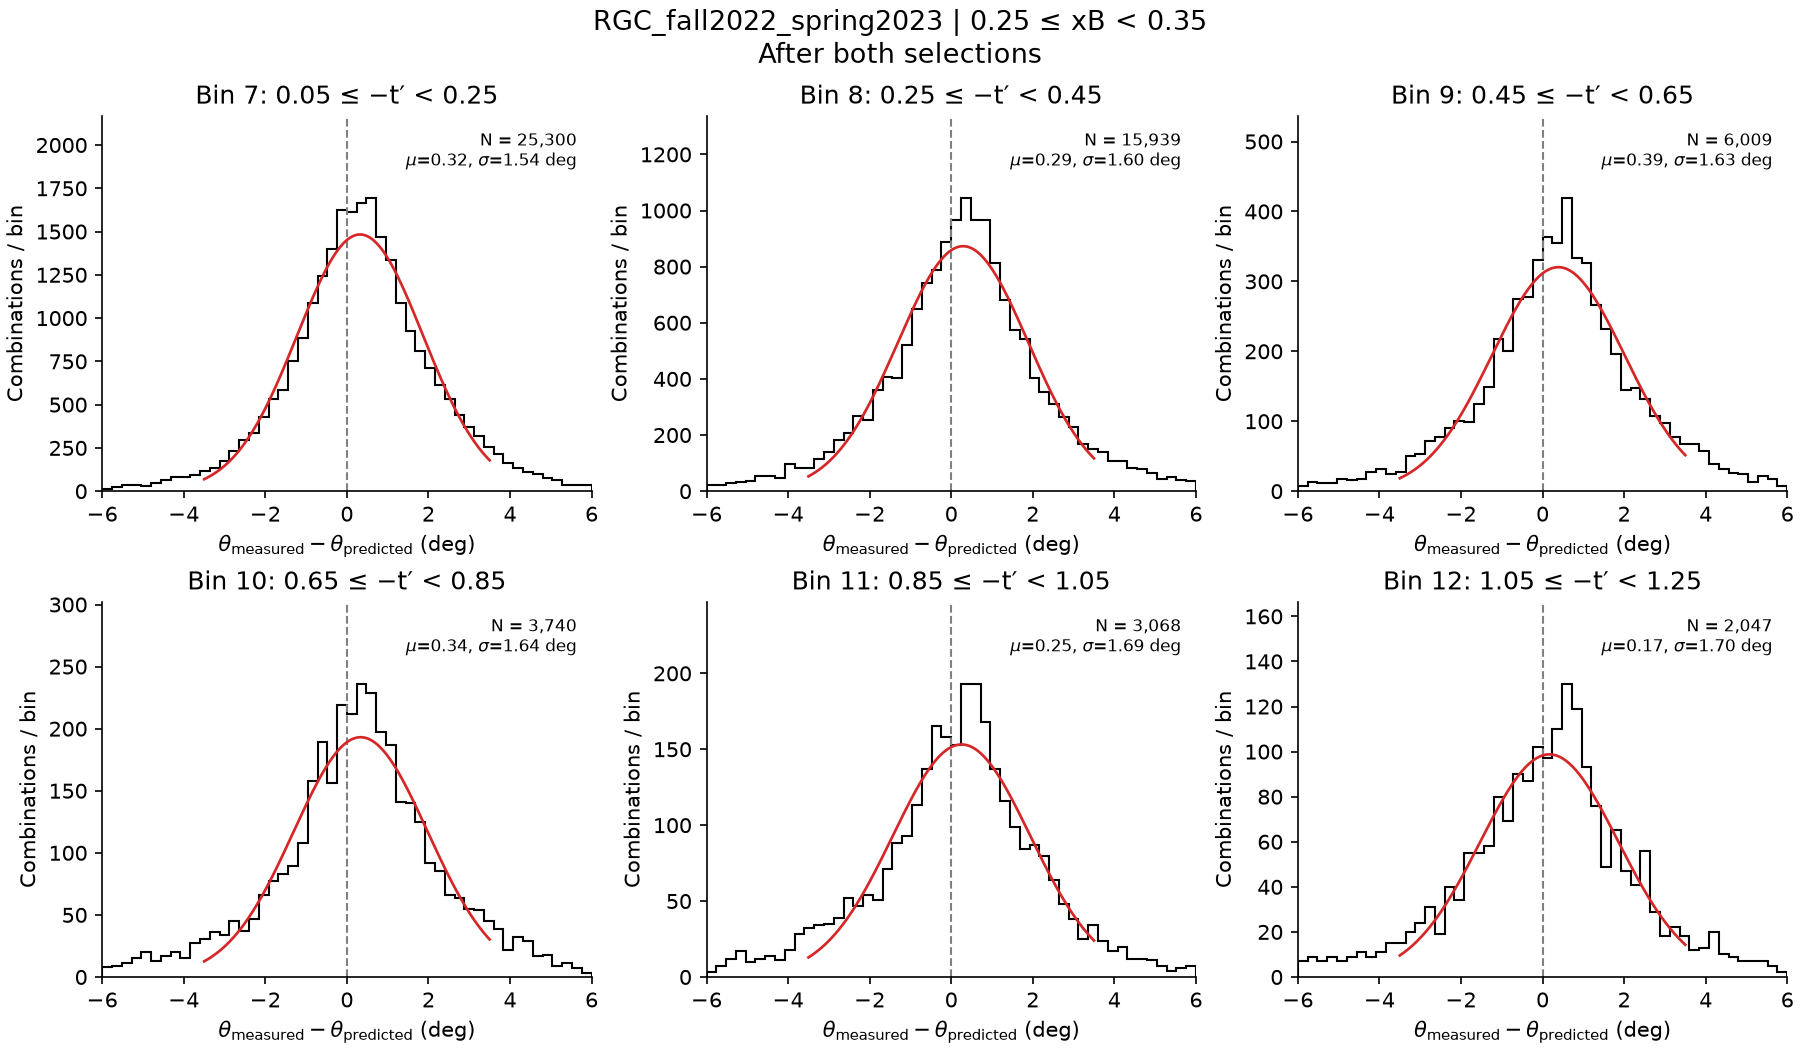
\includegraphics[width=\linewidth]{figures/channel_selection/exclusivity/rgc_fa22_sp23_angle_xb2.png}
\caption{RGC\_fall2022\_spring2023: pion polar-angle closure after both cuts in $x_B$ interval 2. The panels retain the six fine selection bins.}\label{fig:new_excl_rgc_fa22_sp23_angle2}
\end{figure}
\clearpage
\begin{figure}[p]\centering
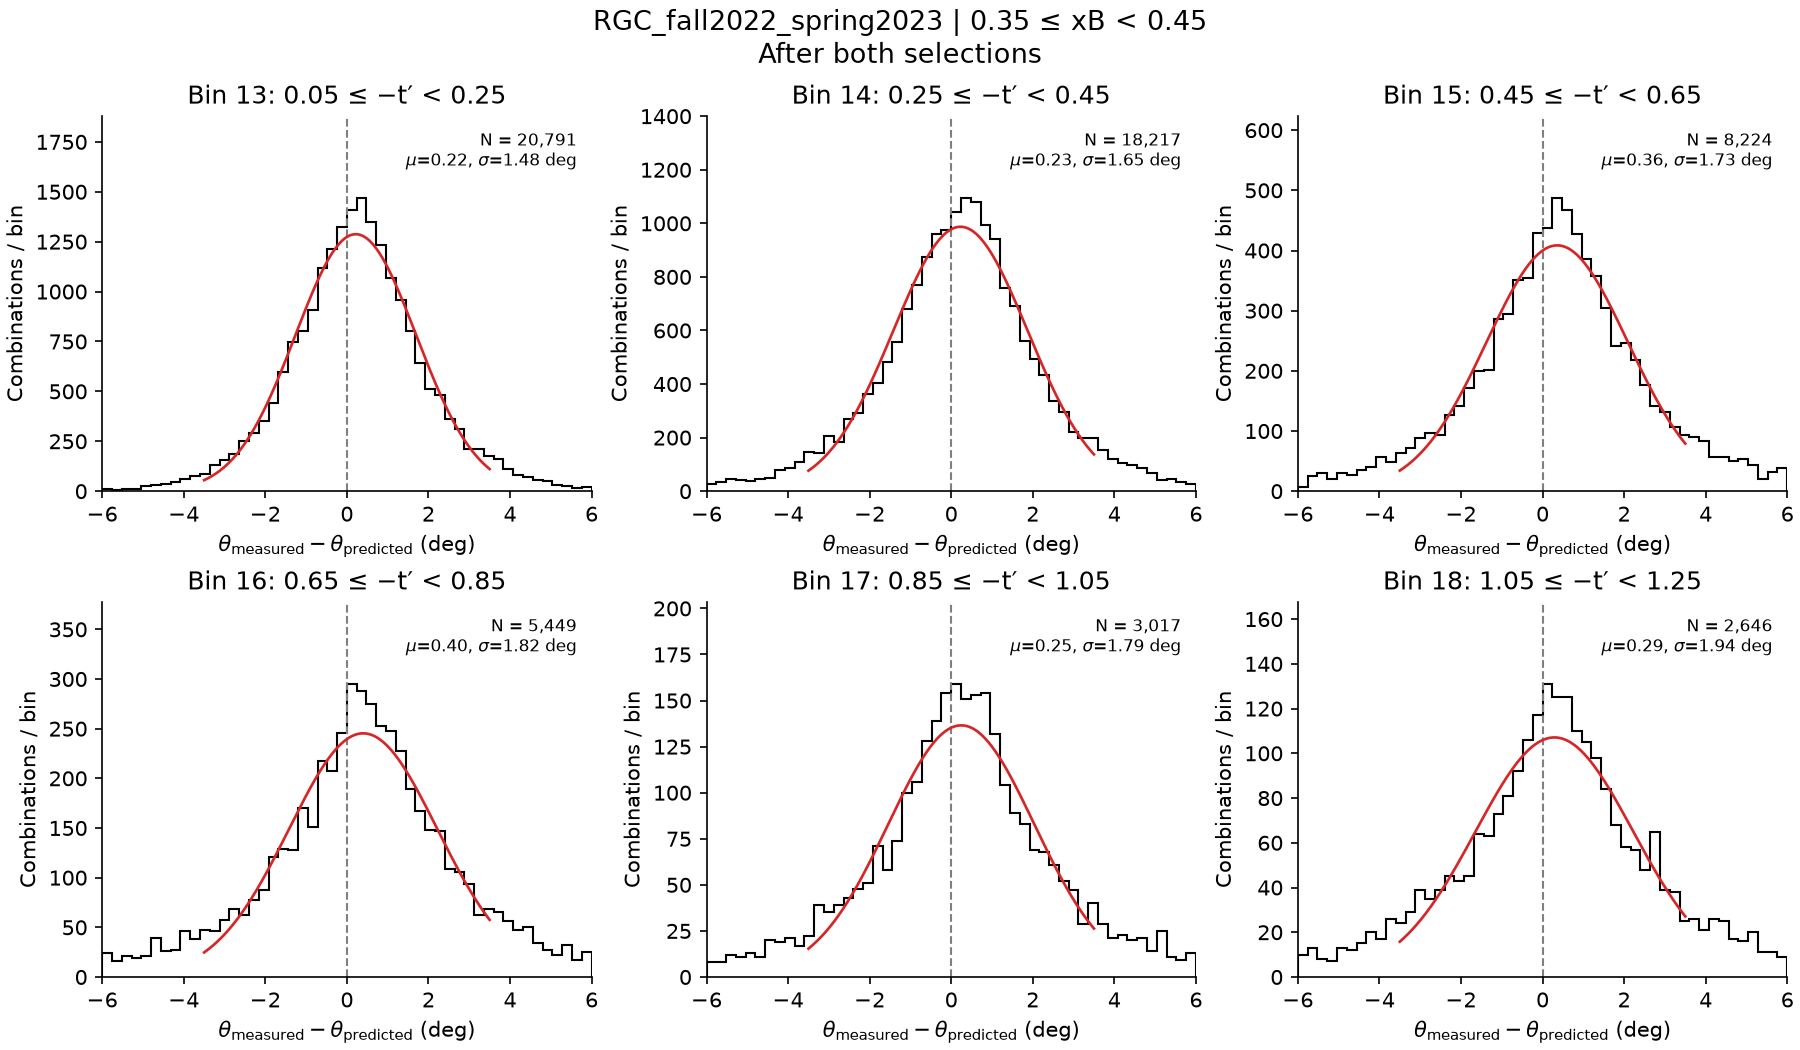
\includegraphics[width=\linewidth]{figures/channel_selection/exclusivity/rgc_fa22_sp23_angle_xb3.png}
\caption{RGC\_fall2022\_spring2023: pion polar-angle closure after both cuts in $x_B$ interval 3. The panels retain the six fine selection bins.}\label{fig:new_excl_rgc_fa22_sp23_angle3}
\end{figure}
\clearpage
\begin{figure}[p]\centering
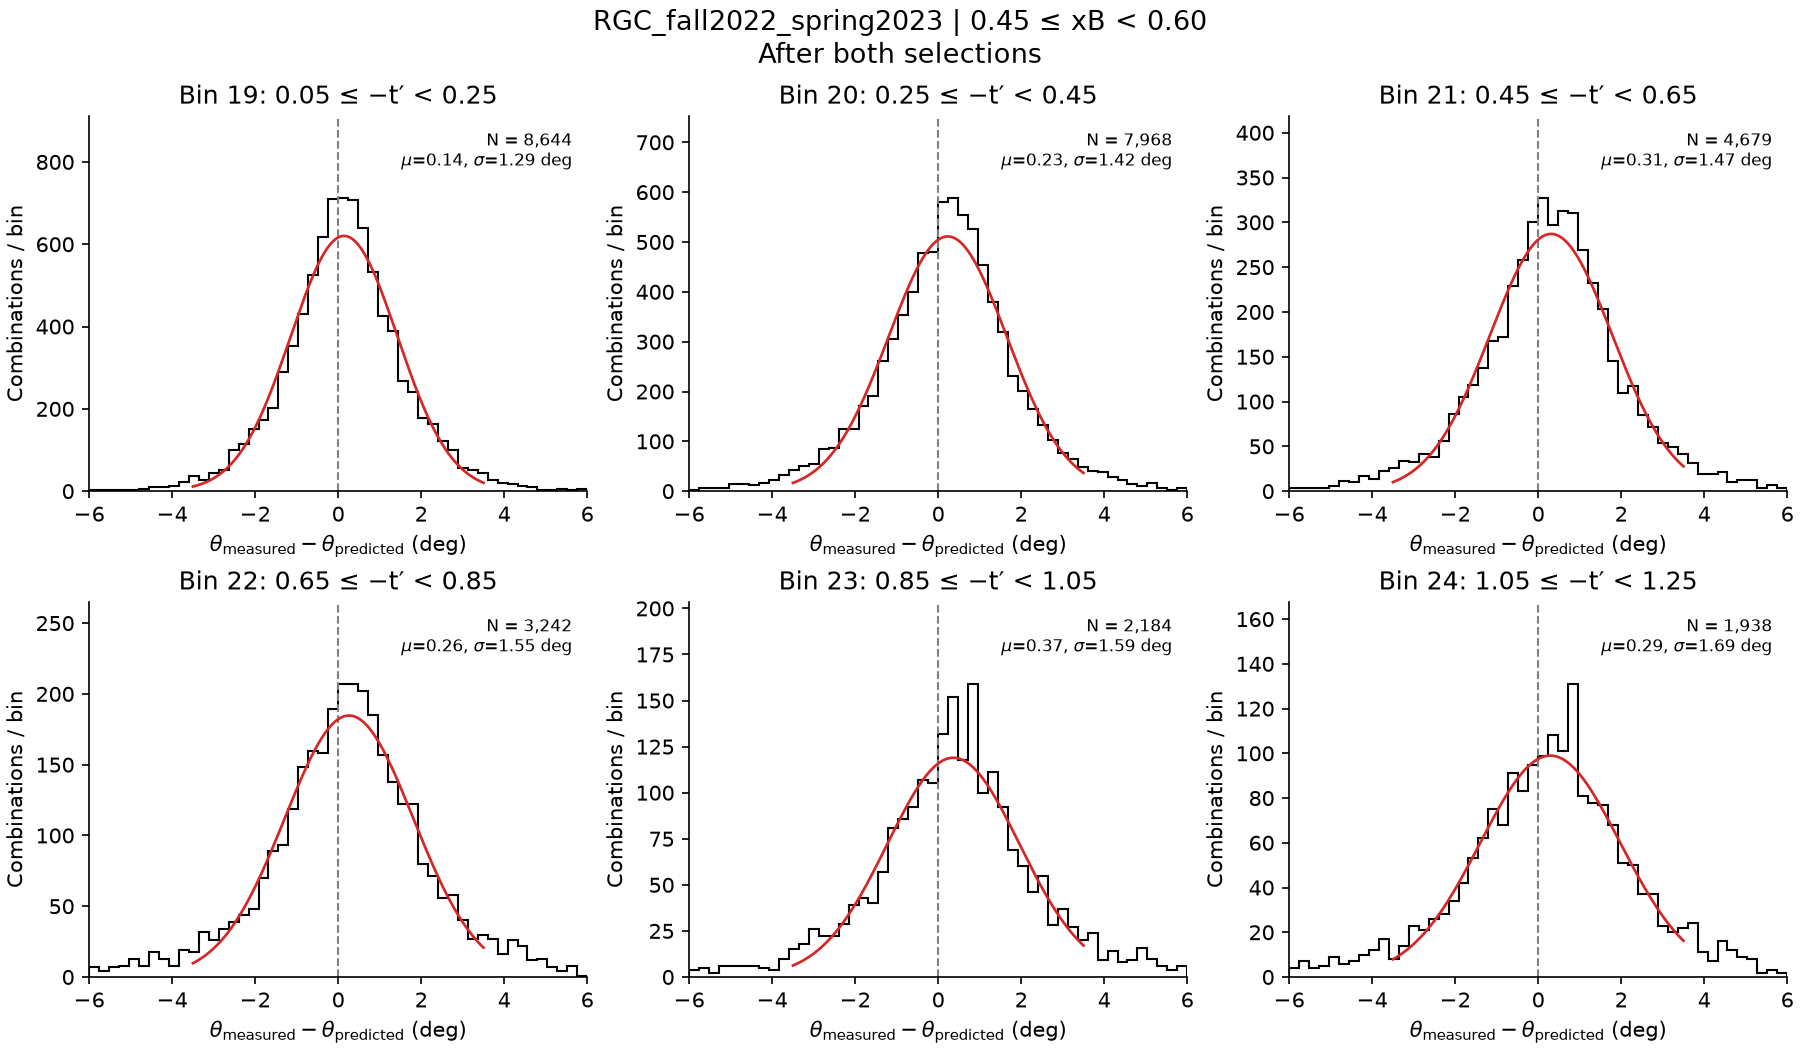
\includegraphics[width=\linewidth]{figures/channel_selection/exclusivity/rgc_fa22_sp23_angle_xb4.png}
\caption{RGC\_fall2022\_spring2023: pion polar-angle closure after both cuts in $x_B$ interval 4. The panels retain the six fine selection bins.}\label{fig:new_excl_rgc_fa22_sp23_angle4}
\end{figure}
\clearpage
